\documentclass[10pt]{article}
% Math Packages
\usepackage{float} % Required to use [H]
\usepackage{amsmath, mathtools}
\usepackage{amssymb}
\usepackage{amsthm}
\usepackage{amsfonts}
\usepackage{bbm}
\usepackage{breqn}
\usepackage[margin=1in]{geometry}
\usepackage{graphicx}
\usepackage{tikz}
\usetikzlibrary{arrows.meta}
\usetikzlibrary{calc}
\usepackage{forest}
\usepackage{tikz-qtree}
\graphicspath{ {./images/} }
\usepackage{hyperref}
\usepackage[capitalize]{cleveref}
\usepackage[shortlabels]{enumitem}
\usetikzlibrary{arrows,matrix,positioning}
\usepackage{multicol}

\usepackage{mathtools}% http://ctan.org/pkg/mathtools
\usepackage{abraces} %xyz



\usepackage{empheq} % for boxed equations
\usepackage[most]{tcolorbox}
\newtcbox{\mymath}[1][]{%
  nobeforeafter, math upper, tcbox raise base,
  enhanced, colframe=blue!30!black,
  colback=blue!30, boxrule=1pt,
  #1}
\newtcbox{\boxmath}[1][]{%
  nobeforeafter, math upper, tcbox raise base,
  enhanced, colframe=blue!30!black,
  boxrule=1pt,
  #1}

% for the pipe symbol
\usepackage[T1]{fontenc}


% Citing theorems by name. (source: https://tex.stackexchange.com/questions/109843/cleveref-and-named-theorems)
\makeatletter
\newcommand{\ncref}[1]{\cref{#1}\mynameref{#1}{\csname r@#1\endcsname}}

\def\mynameref#1#2{%
  \begingroup
  \edef\@mytxt{#2}%
  \edef\@mytst{\expandafter\@thirdoffive\@mytxt}%
  \ifx\@mytst\empty\else
  \space(\nameref{#1})\fi
  \endgroup
}
\makeatother

% Colorful Notes
\usepackage{color} \definecolor{Red}{rgb}{1,0,0} \definecolor{Blue}{rgb}{0,0,1}
\definecolor{Purple}{rgb}{.5,0,.5} \def\red{\color{Red}} \def\blue{\color{Blue}}
\def\gray{\color{gray}} \def\purple{\color{Purple}}
\newcommand{\rnote}[1]{{\red [#1]}} % \rnote{foo} gives '[foo]' in red
\newcommand{\pnote}[1]{{\purple [#1]}} % \pnote{foo} gives '[foo]' in purple
\newcommand{\bnote}[1]{{\blue #1}} % \bnote{foo} gives 'foo' in blue
\newcommand{\gnote}[1]{{\gray #1}} % \gnote{foo} gives 'foo' in gray
\newcommand{\Max}[1]{{\purple [#1]}} % \bnote{foo} then 'foo' is blue


% Claim numbering (the counter restarts after each proof environment)
\newcounter{claimcount}
\setcounter{claimcount}{0}
\newenvironment{claim}{\refstepcounter{claimcount}\par\addvspace{\medskipamount}\noindent\textbf{Claim \arabic{claimcount}:}}{}
\usepackage{etoolbox}
\AtBeginEnvironment{proof}{\setcounter{claimcount}{0}}
\newenvironment{claimproof}{\par\addvspace{\medskipamount}\noindent\textit{Proof of Claim  \arabic{claimcount}.}}{\hfill\ensuremath{\qedsymbol} \tiny{Claim}

  \medskip}
% Add claim support to cleverref
\crefname{claimcount}{Claim}{Claims}


% Math Environments
\newtheorem{theorem}{Theorem}
\newtheorem{assumption}[theorem]{Assumption}
\newtheorem{lemma}[theorem]{Lemma}
\newtheorem{proposition}[theorem]{Proposition}
\newtheorem{corollary}[theorem]{Corollary}
\newtheorem{question}[theorem]{Question}
\theoremstyle{definition}
\newtheorem{definition}[theorem]{Definition}
\newtheorem{remark}[theorem]{Remark}
\newtheorem{example}[theorem]{Example}
\newtheorem{notation}[theorem]{Notation}
\newtheorem{problem}[theorem]{Problem}


\usepackage{skull}

% Redefine the Example environment to include "End of example [number]"
\makeatletter
\let\oldexample\example
\renewenvironment{example}
{\begin{oldexample}}
  {\par\smallskip\hfill   End of Example~\theexample. $\square$    \par\end{oldexample}}
\makeatother


% Matrices and Column Vectors. 
\usepackage{stackengine}
\setstackgap{L}{1.0\normalbaselineskip}
\usepackage{tabstackengine}
\setstackEOL{;}% row separator
\setstackTAB{,}% column separator
\setstacktabbedgap{1ex}% inter-column gap
\setstackgap{L}{1.5\normalbaselineskip}% inter-row baselineskip
\let\nmatrix\bracketMatrixstack  %Usage: \nmatrix{1,2,3\4,5,6}
\newcommand\cv[1]{\setstackEOL{,}\bracketMatrixstack{#1}} %usage: \cv{1,2,3}

% Custom Math Coqmmands
\newcommand{\vt}{\vskip 5mm} % vertical space
\newcommand{\fl}{\noindent\textbf} % first line
\newcommand{\Fl}{\vt\noindent\textbf} % first line with space above
\newcommand{\norm}[1]{\left\lVert#1\right\rVert} % norm
\newcommand{\pnorm}[1]{\left\lVert#1\right\rVert_p} % p-norm
\newcommand{\qnorm}[1]{\left\lVert#1\right\rVert_q} % q-norm
\newcommand{\1}[1]{\textbf{1}_{\left[#1\right]}} % indicator function 
\def\limn{\lim_{n\to\infty}} % shortcut for lim as n-> infinity
\def\sumn{\sum_{n=1}^{\infty}} % shortcut for sum from n=1 to infinity
\def\sumkn{\sum_{k=1}^{n}} % shortcut for sum from k=1 to n
\def\sumin{\sum_{i=1}^{n}} % shortcut for sum from i=1 to n
\def\SAs{\sigma\text{-algebras}} % shortcut for $\sigma$-algebras
\def\SA{\sigma\text{-algebra}} % shortcut for $\sigma$-algebra
\def\Ft{\mathcal{F}_t} % time-indexed sigma-algebra (t)
\def\Fs{\mathcal{F}_s} % time-indexed sigma-algebra (s)
\def\F{\mathcal{F}} % sigma-algebra
\def\G{\mathcal{G}} % sigma-algebra
\def\R{\mathbb{R}} % Real numbers
\def\N{\mathbb{N}} % Natural numbers
\def\Z{\mathbb{Z}} % Integers
\def\E{\mathbb{E}} % Expectation
\def\P{\mathbb{P}} % Probability
\def\Q{\mathbb{Q}} % Q probability
\def\dist{\text{dist}} %Text 'dist' for things like 'dist(x,y)'
\newcommand{\indep}{\perp \!\!\! \perp}  %independence symbol
\def\Var{\mathrm{Var}} % Variance
\def\tr{\mathrm{tr}} % trace

% Brackets and Parentheses
\def\[{\left [}
    \def\]{\right ]}
% \def\({\left (}
%   \def\){\right )}




\usepackage{color}
\definecolor{Red}{rgb}{1,0,0}
\definecolor{Blue}{rgb}{0,0,1}
\definecolor{Purple}{rgb}{.5,0,.5}
\def\red{\color{Red}}
\def\blue{\color{Blue}}
\def\gray{\color{gray}}
\def\purple{\color{Purple}}
\definecolor{RoyalBlue}{cmyk}{1, 0.50, 0, 0}
\newcommand{\dempfcolor}[1]{{\color{RoyalBlue}#1}} 
\newcommand{\demph}[1]{\dempfcolor{{\sl \textbf{#1}}}}

% comment exactly one of the following line to show / hide the solutions
% \newcommand{\solution}[1]{{\purple #1}} % uncomment to show the solutions
\newcommand{\solution}[1]{} % uncomment to hide the solutions



\title{Lecture Notes for Math 372: \\Elementary Probability and Statistics}
\date{Last updated: \today}
% \author{mh}

\begin{document}
\maketitle


\begin{quote}
  \textit{Probability theory has a right and a left hand. On the right is the rigorous foundational work using
    the tools of measure theory. The left hand ``thinks probabilistically,'' reduces problems to gambling
    situations, coin-tossing, models of a physical particle.} -- Leo Breiman
\end{quote}


\tableofcontents
\newpage
\section*{About these notes}

These lecture notes were prepared by Max Hill for a 16-week course on
probability and statistics (MATH 372) at University of Hawaii at Manoa in
Spring 2025. The textbook used is \textit{Probability and Statistics for
  Engineering and the Sciences} (9th edition) by Jay L.~Devore. In addition to
this text, the material in these lecture notes is also based on a number of
other sources as well, including:
\begin{itemize}
  \item Milton and Arndold's \textit{Introduction to Probability and Statistics} (2nd edition) 
  \item D.~Zeilberger's lecture notes \url{https://sites.math.rutgers.edu/~zeilberg/math477/}
  \item Unpublished lecture notes from E.~Gross, R.~Willett, J.~Kim, and B.~Xie.
  \item My notes from when I took probability with W.~Peterson in 2012.
  \item L.~Breiman's \textit{Probability} (1992).
  \item K.L.~Chung's wonderful textbook \textit{Elementary Probability Theory with Stochastic
    Processes}, (1975).
  \item H.~Pishro-Nik's online textbook ``Introduction to Probability,
  Statistics, and Random Processes''
  \item ``Introduction to Probability'' by D.~Anderson, T.~Seppalainen, and B.~Valko.
\end{itemize}
\newpage
\setcounter{section}{-1}
\section{Tentative course outline}

This course is a problem-oriented introduction to the basic concepts of probability and statistics,
providing a foundation for applications and further study.

\begin{itemize}
  \item \textbf{Weeks 1-2:} Introduction to probability theory 
  \begin{itemize}
    \item Experiments, events, sets, probabilities, random variables. Equally likely outcomes, counting
    techniques. Conditional probability. Independence. Bayes' theorem. (Sections: 2.1-2.5)
  \end{itemize}
  \item \textbf{Weeks 3-5:} Random variables
  \begin{itemize}
    \item Discrete random variables (1.5 weeks): Expected values, mean, variance, binomial distribution,
    Poisson distribution. Moment generating functions.  (Sections: 3.1-3.6)
    \item Continuous Random variables (1.5 weeks): Uniform, exponential, gamma, and normal distributions.
    Intuitive treatment of the Poisson process and development of the relationship with gamma
    distributions. (Sections: 4.1-4.4)
  \end{itemize}
  \item \textbf{Midterm 1 (Feb 18)}
  \item \textbf{Weeks 6-7:} Multivariate distributions
  \begin{itemize}
    \item Calculation of probability, covariance, correlation, marginals, conditions. Distributions of
    sums of random variables and sampling distributions. Central limit theorem. (Sections: 1.1, 1.3, 1.4, 5.1-5.7)
  \end{itemize}
  \item \textbf{Week 8:} Catch-up, review.
  \item \textbf{Week 9:} Introduction to statistical estimation
  \begin{itemize}
    \item Point and confidence interval estimation. Maximum likelihood, optimal, and unbiased estimators.
    Examples. (Sections 6.1, 6.2)
  \end{itemize}
  \item \textbf{Midterm 2 (March 27)}
  \item \textbf{Weeks 10-12:} Large sample inference
  \begin{itemize}
    \item Estimation (1.5 weeks): Types and comparison of estimators; sampling distributions
    for means/proportions, and their use in large sample estimation; sample size. (Sections 7.1,
    7.2)
    \item Hypothesis testing (1.5 weeks): Components of a test; signficance and power; p-values;
    large-sample tests for means and proportions (Sections: 8.1-8.4)
  \end{itemize}
  \item \textbf{Week 13:} Small sample inference
  \begin{itemize}
    \item t-distribution, with applications to small sample estimation and testing; $\chi^{2}$ and $F$
    distributions, with applications to inference about variances (Sections: 7.3, 7.4, 8.3)
  \end{itemize}
  \item \textbf{Weeks 14-16:} Regression and $\chi^{2}$ tests
  \begin{itemize}
    \item Regression (1.5 weeks): Least squares, correlation coefficient, inference (Sections:
    12.1-12.5)
    \item $\chi^{2}$ tests: multinomial dsitributions, contingency tables, goodness-of-fit (Sections: 14.1-14.3)
  \end{itemize}
  \item \textbf{Last day of instruction: May 6}
  \item \textbf{Final Exam: May 15}
\end{itemize} 

\newpage
\section{2025-01-12 | Week 01 |  Lecture 01}
\begin{itemize}
  \item give syllabus
  \item do activity with why you're in this course
  \item do the pirates worksheet
\end{itemize}

\newpage
\section{2025-01-14  | Week 01 | Lecture 02}
\begin{center}
  \begin{tcolorbox}[width=0.9\textwidth, colback=white, colframe=black]
    \textit{\textbf{The nexus question of this lecture:} What is the general
      framework for probability?}

    \textit{\textbf{Reading assignment:} chapters 2.1 - 2.5}
  \end{tcolorbox}
\end{center}

\subsection{A general framework for probability}
We begin with a general framework and some terminology to formalize the
notions of probability.

\begin{itemize}
  \item An \demph{experiment} is an activity or process whose outcome is
  subject to uncertainty, and about which an observation is made.

  Examples include flipping a coin, rolling a dice, measuring the size of a
  wave, or the amount of rainfall, conducting a poll, performing a diagnostic
  test, opening a pack of Pokemon cards, etc.

  \item The \demph{sample space} $S$ of an experiment is the set of all
  possible outcomes. The elements of the sample space are called \demph{sample
    points}.

  We think of each sample point as representing a unique outcome of the
  experiment. In the case of rolling a dice, the sample points are $1,2,3,4,5$
  and $6$, and the sample space is $S=\left\{1,2,3,4,5,6\right\}$.


  \item We use the term \demph{event} to refer to a collection of outcomes. So
  we think of an event as being a \textit{subset} of the sample space:
  \begin{equation*}
    \text{an event} = \text{a set of outcomes} = \text{a subset of $S$}.
  \end{equation*}



  Example: if our experiment is rolling a 6-sided dice, here are some events

  \begin{equation*}
    \begin{aligned}
      A &= [\text{observe an odd number}]\\
      B &= [\text{observe an even number}]\\
      C &= [\text{observe a number less than 5}]\\
      D &= [\text{observe a 2 or a 3}]\\
      E_1 &= [\text{observe a 1}]
    \end{aligned}
    \qquad
    \begin{aligned}
      E_2 &= [\text{observe a 2}]\\
      E_3 &= [\text{observe a 3}]\\
      E_4 &= [\text{observe a 4}]\\
      E_5 &= [\text{observe a 5}]\\
      E_6 &= [\text{observe a 6}]
    \end{aligned}
  \end{equation*}

  \item There are two types of events: \demph{compound events}, which can be
  decomposed into other events, and \demph{simple events}, which cannot.

  In the above example, the events $A,B,C$ and $D$ are compound events. $E_{1},\ldots,E_{6}$ are simple events.

  \begin{equation*}
    \begin{aligned}
      A &= [\text{observe an odd number}] = \{1,3,5\} \\
      B &= [\text{observe an even number}] = \{2,4,6\} \\
      C &= [\text{observe a number less than 5}] = \{1,2,3,4\} \\
      D &= [\text{observe a 2 or a 3}] = \{2,3\}\\
      E_1 &= [\text{observe a 1}] = \{1\}
    \end{aligned}
    \qquad
    \begin{aligned}
      E_2 &= [\text{observe a 2}] = \{2\} \\
      E_3 &= [\text{observe a 3}] = \{3\} \\
      E_4 &= [\text{observe a 4}] = \{4\} \\
      E_5 &= [\text{observe a 5}] = \{5\} \\
      E_6 &= [\text{observe a 6}] = \{6\}
    \end{aligned}
  \end{equation*}

\end{itemize}



\begin{example}[Examples of sample spaces]
  \begin{itemize}
    \item[]
    \item If I roll dice, the sample space is $S = \left\{1,2,3,4,5,6\right\}$
    
    \item  If I flip a coin, the sample space is $S = \left\{T,H\right\} $
     
    \item The amount of rainfall in a day is
    $S = \left\{x\in \mathbb{R}: x \geq 0\right\}$
    
    An example of an event for this sample space is:
    \begin{equation*}
      \left[ \text{between 1 and 2 inches of rain} \right]  = \left\{x\in \mathbb{R}: 1 \leq x \leq 2\right\}.
    \end{equation*}

    \item You've got an urn filled with 300,000,000 balls. Exactly one ball is made of gold. Draw a ball
    out at random. If it's not the gold ball, put it back and keep repeating until you get the gold ball.
    Once you get the gold ball, you are done. The output of this experiment is \textit{the number of
      times you drew a ball from the urn}. The sample space is
    \begin{equation*}
      S = \left\{1,2,3,4,\ldots\right\}.
    \end{equation*}
  \end{itemize}
  The last two examples show that the sample space need not be finite.
\end{example}


% \begin{example}[Rolling a dice]
%   To illustrate, suppose we roll a dice. Let $X$ be the value of the dice roll. We know the sample space
%   of the experiment is $S = \left\{1,2,3,4,5,6\right\}$. Some possible events, along with the sets we
%   identify them with, are shown below:
%   \begin{itemize}
%     \item ``the dice roll is even'' \dotfill $\left\{2,4,6\right\}$
%     \item ``the dice roll is at least 3'' \dotfill $\left\{3,4,5,6\right\}$
%     \item ``the dice roll equals 1'' \dotfill $\left\{1\right\}$
%   \end{itemize}
%   It's common to represent events using square brackets like this:
%   $\left[ \text{event description} \right]$. For example, the first event above could also be written as:
%   \begin{equation*}
%     \left[ X \text{ is even} \right] \quad \text{or }\quad \left[ X \in \left\{2,4,6\right\} \right].
%   \end{equation*}
%   And we might write the other two events as
%   \begin{equation*}
%     \left[ X \geq 3\right] \quad \text{and} \quad \left[ X=1 \right].
%   \end{equation*}
% \end{example}
\subsection{The enumeration principle}
\begin{example}[Rolling two dice]
  When rolling a red and a blue dice, the sample space consists of 36 possible outcomes:
  \begin{center}
    \includegraphics[scale=0.3]{images/state-space-2-dice-rolls}
  \end{center}
  so we can write the sample space as:
  \begin{align*}
    S
    &= \left\{(x,y): x,y\in \left\{1,2,3,4,5,6\right\}\right\}\\
    &= \left\{(1,1), (1,2), \ldots, (6,6)\right\}
  \end{align*}
  The event that the dice are equal is
  \begin{equation*}
    \left[ \text{dice are equal} \right]  = \left\{(1,1), (2,2), (3,3), (4,4), (5,5), (6,6)\right\}
  \end{equation*}
  We could have other events too, like that the dice sum to 3:
  \begin{equation*}
    \left[ \text{dice sum to 4}  \right] = \left\{(1,3),(2,2),(3,1)\right\} 
  \end{equation*}

  % Let's do this for all possible sums of our red and blue dice:
  % \begin{center}
  %   \includegraphics[scale=0.5]{images/sums-events.png}
  % \end{center}
  All of the outcome pairs are equally likely, so we can compute the probabilities of by counting entires
  in the table. Let
  \begin{equation*}
    Z = \text{the sum of the red dice and the blue dice}
  \end{equation*}
  By counting entries in our table, we see that
  \begin{equation*}
    \P\left[Z =  4 \right] = \frac{3}{36}.
  \end{equation*}
  Similarly,
  \begin{equation*}
    \P\left[Z = 7 \right] = \frac{6}{36} = \frac{1}{6}
  \end{equation*}
  and
  \begin{equation*}
    \P\left[Z \leq 5\right] = \frac{10}{36}.
  \end{equation*}
\end{example}

The previous example illustrates the critically imporant idea of \textbf{enumeration:}

\begin{center}
  \colorbox{gray!10}{%
    \begin{minipage}{0.8\textwidth}
      If your sample space is finite and consists of \textit{equally likely outcomes}, then you can
      compute lots of probabilities easily by listing outcomes and counting them. To be prcecise, for any
      event $A$,
      \begin{equation*}
        \P\left[A \right] = \frac{|A|}{|S|}  = \frac{\# \text{ of outcomes in $A$ }}{\# \text{ of outcomes in
            $S$ }}
      \end{equation*}
    \end{minipage}%
  }
\end{center}

I already had you do a bunch of these problems on Monday.






\newpage



\subsection{Events}

Some observations about events:
\begin{itemize}
  \item Two events $E$ and $F$ are \demph{mutually exclusive} if
  $E\cap F =\emptyset$. This means that $E$ and $F$ cannot both happen at the
  same time.
  \begin{center}
    \includegraphics[scale=.4]{images/venn-diagram-disjoint}
  \end{center}

  In the dice example, the events $A$ and $B$ are mutually exclusive, since
  the dice roll cannot be both even and odd. But $A$ and $C$ are not mutually
  exclusive because $A\cap C =\left\{1,3\right\}\neq \emptyset$. If a 1 or a 3
  is rolled, then both $A$ and $C$ occur.

  \item The sample points are \textit{elements} of $S$. The simple events
  are \textit{singleton subsets} of $S$. In the dice example, we have:
  \begin{itemize}
    \item Sample points: 1,2,3,4,5,6.
    \item Simple events:
    $\left\{1\right\},\left\{2\right\},\left\{3\right\},\left\{4\right\},\left\{5\right\},\left\{6\right\}$.
  \end{itemize}
  \item The empty set $\emptyset$ and the whole sample space $S$ are always
  both events: $\emptyset$ is the event ``nothing happens'' and $S$ is the
  event ``something happens''.
  \item If $E$ and $F$ are events, then $E\cap F$ is the event that both $E$
  \textbf{and} $F$ occur:
  \begin{center}
    \includegraphics[scale=0.2]{images/venn-diagram-intersection}
  \end{center}
  Here, $E\cap F$ is the \demph{intersection} of $E$ and $F$; that is, $E\cap F$ the set
  of sample points contained in both $E$ and $F$.
  
\end{itemize}

\newpage

\newpage
\section{2025-01-17 | Week 1 | Class 3}
\subsection{Cool coin flipping experiment}
\begin{example}[Cool coin flipping experiment]
  \label{ex:cool-coin-flipping-example}
  Consider the following experiment:
  \begin{enumerate}
    \item Flip a coin.
    \item If the coin is tails, go back to step 1. Otherwise, stop.
  \end{enumerate}
  In other words, we flip a coin repeatedly until we get a heads.
  
  \fl{Output:} the number of times we flipped the coin.

  This experiment is very similar to the example from last lecture in which we had an urn with
  300,000,000 balls, exactly one of which was gold. 

  The sample space is
  \begin{equation*}
    S = \left\{1,2,3,4,\ldots\right\}
  \end{equation*}
  since there is no limit to the number of times we might have to flip the coin before getting a heads!


  Let $X$ be the number of times we flipped the coin. Then
  \begin{equation*}
    \P\left[X = 1 \right] = \P\left[\text{first coin flip was heads} \right] = \frac{1}{2}
  \end{equation*}
  and
  \begin{equation*}
    \P\left[X = 2 \right] 
    = \P\left[\text{first flip was tails and second was heads} \right] 
    = \frac{1}{2}\cdot \frac{1}{2}
    = \frac{1}{4}.
  \end{equation*}
  Similarly,  for any $n=1,2,3,4,\ldots$, we have
  \begin{equation}\label{eq:1}
    \P\left[X=n \right]= \left( \frac{1}{2} \right)^{n} 
  \end{equation}

  How many times do we expect to flip the coin? I mean, what is $\E\left[X \right]$?

  We use the formula
  \begin{equation*}
    \E\left[X \right] = \sum_{n=1}^{\infty}n \P\left[X=n \right] 
  \end{equation*}
  which gives
  \begin{align*}
    \E\left[X \right] 
    =& \sum_{n=1}^{\infty} n \left( \frac{1}{2} \right)^{n} \\
    =& \frac{1}{2} + 2 \left( \frac{1}{2} \right)^{2}+ 3 \left( \frac{1}{2} \right)^{3}+
       4 \left( \frac{1}{2} \right)^{4}+\ldots \\
    =& \frac{1}{2} +  2\cdot \frac{1}{4}+ 3\cdot \frac{1}{8} + 4\cdot \frac{1}{16}+\ldots\\
    =& \frac{1}{2} + \left(\frac{1}{4}+ \frac{1}{4}\right) + \left(\frac{1}{8} + \frac{1}{8} + \frac{1}{8}\right)
       + \left( \frac{1}{16} + \frac{1}{16} + \frac{1}{16} + \frac{1}{16} \right)  + \ldots\\
    =& \frac{1}{2} + \frac{1}{4} + \frac{1}{8} + \frac{1}{16} + \frac{1}{32} +\ldots\\
    &\phantom{ \frac{1}{2}} + \frac{1}{4} + \frac{1}{8} + \frac{1}{16} + \frac{1}{32}+ \ldots\\
    &\phantom{ \frac{1}{2} + \frac{1}{4}} + \frac{1}{8} + \frac{1}{16} + \frac{1}{32}+ \ldots\\
    &\phantom{ \frac{1}{2} + \frac{1}{4} + \frac{1}{8}} + \frac{1}{16} + \frac{1}{32}+ \ldots\\
    &\phantom{ \frac{1}{2} + \frac{1}{4} + \frac{1}{8} + \frac{1}{16}} + \frac{1}{32}+ \ldots\\
  \end{align*}
  The first row adds up to $1$ by the geometric series formula (which says that
  $\sum_{n=1}^{\infty}r^{n} = \frac{r}{1-r}$). The second row adds up to $1/2$ (because it's $1/2$ less
  than the first row). The third row adds up to $1/4$. The fourth adds up to $1/8$. etc. So
  \begin{equation*}
    \E\left[X \right] = 1 + \frac{1}{2} + \frac{1}{4}+\frac{1}{8} + \frac{1}{16}+ \ldots
  \end{equation*}
  and applying the geometric series formula again, we see that
  \begin{equation*}
    \E\left[X \right] = 2.
  \end{equation*}
  In other words, we expect to flip the coin twice.

  This problem was easy to state (and some people guessed the correct answer ahead of time!), but it took
  a lot of technical work to compute the answer. (This sort of interplay between our intuition about games of
  chance, and the sometimes difficult technical work needed to answer questions conclusively, is a large
  part of why I think this topic is so interesting.)
\end{example}

\subsection{Set theory}

\textit{Recall:} The \demph{sample space} of an experiment is the \textit{set} of all possible
\demph{outcomes}. An \demph{event} is a collection of outcomes.
\begin{equation*}
  \text{an event} = \text{a set of outcomes} = \text{a subset of the sample space $S$}
\end{equation*}

Roll a red and a blue dice. The \textbf{sample space} is the set
\begin{equation*}
  S = \left\{(1,1),(1,2),\ldots(6,6)\right\}
\end{equation*}
with 36 ordered pairs. Each ordered pair is an \textbf{outcome}. The \textbf{event} that the dice are equal is the
set
\begin{equation*}
  E = \left\{(1,1),(2,2),(3,3),(4,4),(5,5),(6,6)\right\}
\end{equation*}
And the enumeration principle says that
\begin{equation*}
  \P\left[E \right] = \frac{|E|}{|S|} = \frac{6}{36} = \frac{1}{6}.
\end{equation*}

Since probability theory is formalized in terms of sets, we need to have some intuition about set theory.

\begin{itemize}
  \item Suppose $A$ is an event. It's a subset of $S$, like this:
  \begin{center}
    \includegraphics[scale=0.4]{images/venn-diagram-single-event}
  \end{center}
  \item Define the complmenent of $A$: $A'$ or $A^{c}$. [see diagram above]
  \item Suppose $B$ is also an event. We write $A\cup B$ to denote the set of all outcomes that are in
  $A$ or $B$ this includes outcomes that are in both):
  \begin{center}
    \includegraphics[scale=0.3]{images/venn-diagram-union}
  \end{center}
  \item Do the same with $A\cap B$
  \begin{center}
    \includegraphics[scale=0.3]{images/venn-diagram-intersection}
  \end{center}
  \item What if $A$ and $B$ don't overlap at all? In that case, their intersection has nothing in it!
  \begin{center}
    \includegraphics[scale=0.5]{images/venn-diagram-disjoint}
  \end{center}
  In this case, we say that $A\cap B$ is the ``empty set'', which is the set containing no elements. We
  use the symbol $\emptyset$ to represent the empty set; that is,
  \begin{equation*}
    \emptyset := \left\{\right\}
  \end{equation*}
  This is sometimes called the \demph{null event}. If $A\cap B = \emptyset$, then we say that $A$ and $B$
  are \demph{mutually exclusive}, or \demph{disjoint}. For example, if I roll a dice, the events
  \begin{equation*}
    [ \text{dice is even}] \quad \text{and} \quad \left[ \text{dice is odd} \right] 
  \end{equation*}
  are mutually exclusive: they cannot happen simultaneously. 
  \item A sequence of events $\left\{E_{1},E_{2},\ldots\right\}$ is said to be \demph{pairwise disjoint}
  if and only if
  \begin{equation*}
    E_{i}\cap E_{j} = \emptyset \quad \text{ whenever }i\neq j.
  \end{equation*}
  In other words, none of the events in $E$ ``overlap'' with any other events. For an example of this,
  consider the experiment of \cref{ex:cool-coin-flipping-example}, where $X$ is the number of times we
  flip the coin in the experiment. Let
  \begin{equation*}
    E_{n} = \left[ X=n \right] \text{ for }n=1,2,3,\ldots
  \end{equation*}
  Then $\left\{E_{1},E_{2},\ldots\right\}$ is a pairwise disjoint sequence of events.
\end{itemize}



\subsection{Probability Axioms}

A \demph{probability measure} $\P$ is a function which assigns to each event a probability. We denote the
probability of an event $E$ by
\begin{equation*}
  \P\left[E \right] \quad \text{or} \quad  \P\left( E\right).
\end{equation*}
To be a \demph{probability measure}, $\P$ must satisfy the following three axioms:
\begin{enumerate}[label=\textbf{A.\arabic*}]
  \item (Nonnegativity) \label{item:probability-axiom-nonnegativity} For every event $E$, we have
  \begin{equation*}
    \P\left[E\right] \geq 0.
  \end{equation*}
  \item (Sum-to-one) \label{item:probability-axiom-total-measure-one} $\P\left[S \right] =1$
  \item (Countable additivity) \label{item:probability-axiom-countable-additivity} Let
  $E_{1},E_{2},\ldots$ be an infinite sequence of events. If the sequence is pairwise disjoint, then
  \begin{equation*}
    \P\left[E_{1}\cup E_{2}\cup \ldots \right] = \P\left[E_{1} \right]+\P\left[E_{2} \right]+\ldots.
  \end{equation*}
\end{enumerate}
\begin{example}[\cref{ex:cool-coin-flipping-example} continued]
  
  As an example of \ref{item:probability-axiom-countable-additivity}, consider the experiment from
  \cref{ex:cool-coin-flipping-example}, where we had
  \begin{equation*}
    X= \text{(number of coin flips)}.
  \end{equation*}
  For each $n=1,2,\ldots$, define the event $E_{n}$ as
  \begin{equation*}
    E_{n} = \left[ X=n \right].
  \end{equation*}
  We already know that $\P\left[E_{n} \right]= \left(\frac{1}{2}\right)^{n}$ from \cref{eq:1}. Also, you
  should verify for yourself that the sequence
  \begin{equation*}
    \left\{E_{1},E_{2},E_{3},\ldots\right\}
  \end{equation*}
  is pairwise disjoint.

  Now, let's say we want to know the probability that $X$ is even. Observe that
  \begin{equation*}
    \left[ X \text{ is even} \right] = E_{2}\cup E_{4}\cup E_{6}\cup E_{8}\cup\ldots
  \end{equation*}
  Next we will use \ref{item:probability-axiom-countable-additivity} to compute the probability of this event:

  \begin{align*}
    \P\left[X \text{ is even} \right] 
    &= \P\left[E_{2}\cup E_{4}\cup E_{6}\cup E_{8}\cup\ldots \right]\\
    &= \P\left[E_{2} \right] + \P\left[E_{4} \right] + \P\left[E_{6} \right] + \P\left[E_{8} \right] +
      \ldots &&\text{(by \ref{item:probability-axiom-countable-additivity}) }\\
    &= \left( \frac{1}{2} \right)^{2}+\left( \frac{1}{2} \right)^{4}+\left( \frac{1}{2} \right)^{6}+\left(
      \frac{1}{2} \right)^{8}+\ldots &&\text{(by \cref{eq:1}) }\\
    &= \frac{1}{4}+\left( \frac{1}{4} \right)^{2}  + \left( \frac{1}{4} \right)^{3} + \left( \frac{1}{4} \right)^{4}+\ldots\\  
    &= \frac{\frac{1}{4}}{1-\frac{1}{4}} &&\text{ by the geometric series formula $\sum_{n=1}^{\infty}r^{n} = \frac{r}{1-r} $ }\\
    &= \frac{1}{3}. 
  \end{align*}
  So the probability that you flip the coin an \textit{even} number of times is only $1/3$. 
\end{example}
\newpage
\subsection{Understanding ``Events''}

\begin{itemize}
  \item If $E$ and $F$ are events, then $E\cap F$ is the event that both $E$
  \textbf{and} $F$ occur:
  \begin{center}
    \includegraphics[scale=0.2]{images/venn-diagram-intersection}
  \end{center}
  \item If $E$ and $F$ are events, then $E\cup F$ is the event that $E$
  \textbf{or} $F$ occurs.
  \begin{center}
    \includegraphics[scale=0.2]{images/venn-diagram-union}
  \end{center}
  \item If $A$ is an event, then $A^{c}= S\backslash A$ is the event that $E$
  does \textbf{not} occur.
  \begin{center}
    \includegraphics[scale=0.34]{images/venn-diagram-single-event}
  \end{center}
\end{itemize}
\begin{example}[Powerball Lottery]
  \label{ex:powerball-lottery}
  The a ticket for the powerball lottery costs \$2. There are two outcomes:
  \begin{itemize}
    \item You win \$300,000,000.
    \item You don't win any money.
  \end{itemize}
  The probability of winning is approximately $\frac{1}{300,000,000}$. Let $X$ be the net payoff from the
  game, in dollars:
  \begin{itemize}
    \item If you lose, then $X=-2$, since you had to pay \$2 to play the game.
    \item If you win, then your net payoff is $X=299,999,998$. 
  \end{itemize}
  What is the expected value of $X$?
  \begin{align*}
    \E\left[X \right]
    &=\P\left[ \text{win}\right]\cdot (-2) + \P\left[\text{lose} \right]\cdot (299,999,998)\\
    &=\frac{299,999,999}{300,000,000}(-2)+ \frac{1}{300,000,000}(299,999,999)\\
    &=-1.
  \end{align*}
  \textit{Conclusion:} you ``expect'' to lose \$1 every time you play. Similarly, if you play twice, you
  expet to lose \$2. If you play 10 times, you expect to lose \$10. Etc. This property is called
  \textit{linearity} of expectation. 
\end{example}



\begin{itemize}
  \item Go over problem 4, parts (b) and (c). This is the problem where you look ath te expected value of
  2 or 120 dice.
  \item Go over problem 6.
  \item I'll put problems 7 and 8 on the first homework.
  \item ``Elementary'' doesn't mean easy. 
\end{itemize}

\newpage
\section{2025-01-22 |  Week 2 | Class 4}
Recall, a \demph{probability measure} $\P$ is a function which assigns to each possible event a
probability, so that the probability of an event $E$ is denoted $\P\left[E \right]$ or $\P\left(E \right)$. The following axioms hold:
\begin{enumerate}[label=\textbf{A.\arabic*}]
  \item (Nonnegativity) \label{item:probability-axiom-nonnegativity} For every event $E$, we have
  \begin{equation*}
    \P\left[E\right] \geq 0.
  \end{equation*}
  \item (Sum-to-one)  $\P\left[S \right] =1$
  \item (Countable additivity) Let
  $E_{1},E_{2},\ldots$ be an infinite sequence of events. If the sequence is pairwise disjoint, then
  \begin{equation*}
    \P\left[E_{1}\cup E_{2}\cup \ldots \right] = \P\left[E_{1} \right]+\P\left[E_{2} \right]+\ldots.
  \end{equation*}
\end{enumerate}
recall that paiwise dijoint means that there is no overlap.


\begin{proposition}[Basic properties of probability measure]
  \label{prop:some-deductions-from-axioms}
  \begin{enumerate}[label=\rm{(\roman*.)}]
    \item []
    \item (The null event has probability zero) \label{item:empty-set-has-prob-zero}
    $\P\left[\emptyset \right] = 0$
    \item (Finite additivity) \label{item:finite-additivity} Let $\left\{E_{1},\ldots,E_{n}\right\}$ be a
    \textit{finite} sequence of events. If the sequence is pairwise disjoint, then
    \begin{equation*}
      \P\left[E_{1}\cup E_{2}\cup\ldots\cup E_{n} \right] 
      = \P\left[E_{1} \right]+\P\left[E_{2} \right]+\ldots+\P\left[E_{n} \right]
    \end{equation*}
    \item (``With probability one, an event $E$ either does occur or doesn't'') \label{item:complements} $\P\left[E^{c} \right] = 1-\P\left[E \right]$
    \item (Excision Property) \label{item:excision-property} If $A,B$ are events and $A\subseteq B$, then
    \begin{equation*}
      \P\left[B\backslash A \right] = \P\left[B \right] - \P\left[A \right].
    \end{equation*}
    \item (``The particular is less likely than the general'') \label{item:subsets} If $A,B$ are events and $A\subseteq B$, then
    $\P\left[ A\right] \leq \P\left[B \right]$
    \item (``Probabilities are between 0 and 1'') \label{item:probabilities-are-in-unit-interval} For any event $E$,  $\P\left[E \right]\in [0,1]$
  \end{enumerate}
\end{proposition}
\begin{proof}[Proof of \cref{prop:some-deductions-from-axioms}]
  First we will prove \ref{item:empty-set-has-prob-zero}. Let $E_{i}=\emptyset$ for all $i=1,2,3,...$.
  Then
  \begin{itemize}
    \item $\left\{E_{1},E_{2},\ldots\right\}$ is a pairwise disjoint sequence.
    \item If $E_{1}\cup E_{2}\cup\ldots = \emptyset$.
  \end{itemize}
  Therefore,
  \begin{align*}
    \P\left[\emptyset \right] 
    &= \P\left[E_{1}\cup E_{2}\cup\ldots \right]\\
    &= \P\left[E_{1} \right]+ \P\left[E_{2} \right]+\ldots
    &&\text{by \ref{item:probability-axiom-countable-additivity} }\\
    &= \P\left[\emptyset \right]+ \P\left[\emptyset \right]+\ldots.
  \end{align*}
  This equation implies $\P\left[\emptyset \right] = 0$. We have now proved
  \ref{item:empty-set-has-prob-zero}.


  Next we prove \ref{item:finite-additivity}. Let $E_{1},\ldots,E_{n}$ be a finite sequence of events
  which are pairwise disjoint.  Then expand the sequence by taking $E_{i} = \emptyset$ for all $i\in
  \left\{n+1,n+2,\ldots\right\}$. Then by \ref{item:probability-axiom-countable-additivity},
  \begin{align*}
    \P\left[\bigcup_{i=1}^{n}E_{i} \right]\\
    &=\P\left[ \bigcup_{i=1}^{\infty} E_{i}\right] \\
    &= \sum_{i=1}^{\infty} \P\left[E_{i} \right] \\
    &= \P\left[E_{1} \right] + \ldots \P\left[E_{n} \right] +
      \underbrace{\P\left[\emptyset \right] + \P\left[\emptyset \right]+\ldots}
      _{=0\text{by\cref{prop:some-deductions-from-axioms} \ref{item:empty-set-has-prob-zero}}}\\
    &=\P\left[E_{1} \right] + \ldots \P\left[E_{n} \right].
  \end{align*}

  Next we prove \ref{item:complements}. Let $E$ be any event. Then
  \begin{align*}
    1 
    &= \P\left[S \right]  &&\text{by \ref{item:probability-axiom-total-measure-one} }\\
    &= \P\left[ E\cup E^{c}\right] &&\text{since }S = E\cup E^{c}\\
    &= \P\left[E \right]+ \P\left[E^{c} \right]
                          &&\text{by
                             \cref{prop:some-deductions-from-axioms}~\ref{item:finite-additivity},
                             since $E\cap E^{c}=\emptyset$.}
  \end{align*}
  This proves \ref{item:complements}.

  Next we prove \ref{item:excision-property}. Observe that
  \begin{align*}
    B 
    &= (B\cap A) \cup (B\cap A^{c})\\
    &= A \cup B\cap A^{c} &&\text{since $A\subseteq B$.}
  \end{align*}
  This is a disjoint union. Therefore by \ref{item:finite-additivity},
  \begin{align*}
    \P\left[B \right] 
    &= \P\left[A \right] + \P\left[B\cap A^{c} \right]\\
    &= \P\left[A \right] + \P\left[B\backslash A \right].
  \end{align*}
  Rearranging terms proves \ref{item:complements}. 
  Next we prove \ref{item:subsets}. Assume $A\subseteq B$. Then by \ref{item:excision-property},
  \begin{equation*}
    \P\left[B\backslash A \right] = \P\left[B \right] - \P\left[A \right]
  \end{equation*}
  Moreover, by \ref{item:probability-axiom-nonnegativity}, $\P\left[B\backslash A \right] \geq 0$.
  Hence
  \begin{equation*}
    0 \leq  \P\left[B \right] - \P\left[A \right]
  \end{equation*}
  and this implies \ref{item:subsets}.
  
  Finally, we will show \ref{item:probabilities-are-in-unit-interval}. Let $E$ be an event. Then
  \begin{align*}
    0 
    &\leq \P\left[E \right] \leq  \P\left[S \right] \leq &&\text{by \ref{item:probability-axiom-nonnegativity} }\\
    &\leq  \P\left[S \right] &&\text{by \ref{item:subsets} }\\
    &=1 &&\text{by \ref{item:probability-axiom-total-measure-one}. }
  \end{align*}
\end{proof}

\begin{proposition}[Inclusion-Exclusion Prinicple]
  \label{prop:inclusion-exclusion-principle}
  $\P\left[A\cup B \right] = \P\left[A \right]+\P\left[B \right]- \P\left[A\cap B \right]$

  \textit{Idea:}
  \begin{center}
    \includegraphics[scale=1]{images/venn-diagram-union-2}
  \end{center}

\end{proposition}


\begin{proposition}[De Morgan's Laws]
  \label{prop:de-morgans-laws}
  The following equalities hold:
  \begin{equation*}
    \left( A\cup B \right)^{c} = A^{c}\cap B^{c}
    \quad \text{and} \quad 
    \left( A\cap B \right)^{c} = A^{c}\cap B^{c}.
  \end{equation*}
\end{proposition}

\begin{proposition}[Distributive Laws]
  \label{prop:distributive-laws}
  The following equalities hold:
  \begin{equation*}
    A\cup \left( B\cap C \right) = \left( A\cup B  \right)\cap \left( A\cup C \right)  
  \end{equation*}
  and
  \begin{equation*}
    A\cap \left( B\cup C \right) = \left( A\cap B  \right)\cup \left( A\cap C \right)  
  \end{equation*}
\end{proposition}
\subsection{Introduction to counting techniques}
A \demph{k-tuple} is an ordered list of $k$ numbers.

\begin{example}[tuples]
  Consider the experiment in which you roll a dice 5 times in a row:

  \begin{equation*}
    (1,4,6,4,4)
  \end{equation*}
  is a $5$-tuple.

  \fl{Problem:} What is the sample space? How many elements does it have?

  Idea: we will use the \demph{the product rule for $k$-tuples}: 
  \begin{itemize}
    \item there are 6 choices for the first entry
    \item 6 choices for the second entry
    \item $\vdots $ 
    \item 6 choices for the fifth entry
  \end{itemize}
  so the number of possible outcomes is
  \begin{equation*}
    6\times 6 \times 6 \times 6 \times 6 = 6^{5 } = 7776.
  \end{equation*}

  \textbf{Problem:} Let $E = \left[ \text{All 5 dice are less than or equal to 3} \right]$. What is
  $\P\left[E \right]?$

  By the counting principle,
  \begin{equation*}
    \P\left[E \right] = \frac{|E|}{|S|} = \frac{\text{\# ways that all dice are $\leq 3$ }}{7776}
  \end{equation*}
  now we use again the product rule to count the $k$-tuples with all entries less than $3$:
  \begin{equation*}
    3\times 3 \times 3 \times 3 \times 3 = 3^{5} = 243
  \end{equation*}
  So
  \begin{equation*}
    \P\left[E \right] = \frac{243}{7776} = \frac{1}{32}
  \end{equation*}
\end{example}

\newpage
\section{2025-01-24 | Week 2 | Lecture 5}

\subsection{St. Petersburg Paradox}

The game is the following: repeatedly flip a coin until you get heads. You win $2^{n}$ dollars, where $n$ is
the number of coin flips. How much would you be willing to pay to play this game????

Let $X$ be your (random) payoff. The sample space of $X$ is
\begin{equation*}
  S = \left\{2,4,8,16,32,\ldots\right\}.
\end{equation*}
What is the expected value of $X$?

\begin{align*}
  \E\left[X \right] 
  &= \sum_{n=1}^{\infty} n \P\left[X=n \right]\\
  &= \P\left[X=1 \right]+ 2 \P\left[X=2 \right] + 3\P\left[X=3 \right] + 4 \P\left[X=4 \right]
    + 5 \P\left[X=5 \right]
    + 6 \P\left[X=6 \right]
    + 7 \P\left[X=7 \right]\\
  & \quad
    + 8 \P\left[X=8 \right]
    + 9 \P\left[X=9 \right] + \ldots\\
  &= 2 \P\left[X=2 \right] + 4 \P\left[X=4 \right] + 8\P\left[X=8 \right] + 16 \P\left[X=16 \right] +\\
  &= \sum_{k=1}^{\infty} 2^{k}\P\left[X=2^{k} \right] 
\end{align*}
where the third equality follow because $\P\left[X=i \right]=0$ whenever $i\notin S$.


Next, we observe that $\P\left[X=2^{k} \right] = \frac{1}{2^{k}}$ (check this for, say, $k=1,2,3$).

Plugging these probabilities in, we get 

\begin{equation*}
  \E\left[X \right] = \sum_{k=1}^{\infty}2^{k}\cdot \frac{1}{2^{k}} = \sum_{k=1}^{\infty}1 = 1+1+1+1+1+\ldots   = +\infty.
\end{equation*}
The expected value of playing this game is positive infinity!!!!! 


\subsection{Counting Techniques}
There are three main counting principles we'll look at today:
\begin{itemize}
  \item multiplication principle
  \item permutation principle
  \item combination principle
\end{itemize}

Recall that a $k$-tuple is an ordered list of things (usually but not always numbers). A $k$-tuple can
have repeats!


\begin{proposition}[Multiplication Principle]
  Suppose $S$ consist of $k$-tuples and there are $n_{1}$ choices for the first element, $n_{2}$ choices
  for the second, etc. Then there are
  \begin{equation*}
    n_{1}\times n_{2}\times n_{k}
  \end{equation*}
  possible $k$-tuples.
\end{proposition}

\begin{example}
  I roll my lucky dice, flip a gold coin, then flip a silver coin. How many possible outcomes are there?

  [draw a tree to illustrate the product rule]
  \begin{equation*}
    6 \times 2 \times 2 = 24
  \end{equation*}
\end{example}

\begin{example}
  How many ways are there to order the $3$ letters $A,B,C$?

  Use the multiplication principle
  \begin{equation*}
    3 \times 2 \times 1
  \end{equation*}
\end{example}

\begin{proposition}[Counting permutations]
  The total number of ways to order $n$ distinct objects is
  \begin{equation*}
    n! = n \times (n-1)\times(n-2)\times\cdots\times 2 \times 1.
  \end{equation*}
  Each ordering is called a \demph{permutation}. (Note that we define $0! = 1.$)

  (Permutations don't have repeats).
\end{proposition}


\begin{definition}[set]
  A \demph{set} is an \textit{unordered} collection of elements, all of which are \textit{distinct.}
  \begin{itemize}
    \item $\left\{1,2,4,5,3\right\}$ is a set
    \item $\left\{1,1,2,4,5,3\right\}$ is not a set
  \end{itemize}
\end{definition}

\begin{proposition}[Counting subsets -- this is the ``combination principle'']
  Let $S$ be a set with $n$ elements. The number of (unordered) subsets of size $k$ is
  \begin{equation*}
    {n\choose k} =  \frac{n!}{k!(n-k)!}
  \end{equation*}
\end{proposition}


\begin{example}
  Let $S = \left\{1,2,3,4,5,6\right\}$. How many subsets of size 2 are there?

  \begin{equation*}
    {6\choose 2} = \frac{6!}{2! \cdot 4!} = \frac{6\cdot5\cdot4\cdot3\cdot2\cdot1}{\left(2\cdot1\right) \cdot \left(4\cdot3\cdot2\cdot1\right)} = \frac{6\cdot5}{2} = 15.
  \end{equation*}
  These are
  \begin{gather*}
    \left\{1,2\right\}, \left\{1,3\right\}, \left\{1,4\right\}, \left\{1,5\right\}, \left\{1,6\right\} \\
    \left\{2,3\right\}, \left\{2,4\right\}, \left\{2,5\right\}, \left\{2,6\right\} \\
    \left\{3,4\right\}, \left\{3,5\right\}, \left\{3,6\right\} \\
     \left\{4,5\right\}, \left\{4,6\right\} \\
      \left\{5,6\right\}
  \end{gather*}
  note that the order doesn't matter, i.e., $\left\{2,1\right\}=\left\{1,2\right\}$ so this just counts
  as one, not two.

\end{example}

\begin{example}[Poker]
  A poker hand consist of 5 randomly chosen cards from a
  standard 52-card deck.
  \begin{center}
    \includegraphics[scale=0.5]{images/52-card-deck}
  \end{center}
  \fl{Some questions about poker hands:}
  \begin{enumerate}
    \item How many distinct poker hands are there?

    \begin{equation*}
      {52\choose 5} = \frac{52!}{5!\cdot47!} = 2,598,960
    \end{equation*}
    \item How many ways are there to get a flush (i.e., all the same suit)?
    \begin{equation*}
      4 \times {13\choose 5} 
      = 4\cdot \frac{13!}{5! 8!} 
      = 4\cdot\frac{13\cdot 12\cdot 11 \cdot 10 \cdot 9}{5\cdot4\cdot3\cdot2\cdot1} 
      = 5148
    \end{equation*}

    The 4 is to choose a suit. Then we choose 5 out of 13 cards in that suit.
    \item What's the probability that we are dealt a hand in which this occurs? (i.e., in which all cards
    are of the same suit?)

    To answer this, we use the enumeration principle:
    \begin{equation*}
      \frac{{4\choose 1}\times {13\choose 5}}{{52\choose 5}} = \frac{5,148}{2,598,960} \approx 0.002
    \end{equation*}

    In other words, the probability of a flush is pretty low: about $0.2\%$. 
  \end{enumerate}
\end{example}
\newpage

\section{2025-01-27 | Week 3 | Lecture 6}


\subsection{Conditional probability}
\textit{This lecture is based on section 2.4 in the text.}


First, play craps.

Tallying the results, we saw that shooters won about 50\% of the time. Is this a fair game? We will set
out to answer this question. To do so, we'll need to introduce some new ideas. A key idea is that of
conditional probability:


\begin{definition}[Conditional Probability]
  \label{def:conditional-probability}
  Let $A,B$ be events, and assume that $\P\left[A\right]>0$. Then the \demph{conditional probability of
    $B$, given $A$}, denoted $\P\left[B\mid A \right]$, is given by the formula
  \begin{equation*}
    \P\left[B\mid A \right] := \frac{\P\left[A\cap B \right]}{\P\left[A \right]}.
  \end{equation*}
\end{definition}
[draw picture]
\begin{itemize}
  \item Intuitively, $\P\left[B\mid A \right]$ is the probability of $B$ when we know that the event $H$
  as occurred.
  \item The idea is that if we know that event $A$ has occured, then the sample space becomes $A$, and
  the new event is $A\cap B$.
\end{itemize}

For example, 


\begin{example}[Conditional probability]
  I roll a dice behind a screen. I tell you that I rolled an even number. What's the probability that the
  dice roll is a $4$ or a $6$?

  \noindent \textit{Solution:} We have $S = \left\{1,2,3,4,5,6\right\}$, $A= \left\{2,4,6\right\}$,
  $B= \left\{4,6\right\}$. We want to compute $\P\left[B\mid A \right]$. By \cref{def:conditional-probability},
  \begin{equation*}
    \P\left[B\mid A \right] 
    = \frac{\P\left[AB \right]}{\P\left[A \right]} 
    = \frac{2/6}{1/2} 
    = \frac{2}{3}.
  \end{equation*}
  Put differently, we have three outcomes in $A$, which are all equally likely. Two of them (4 and 6)
  mean that event $B$ occurs. So by the enumeration principle, the probability is $2/3$.
\end{example}


Then we worked on \texttt{worksheet-02.pdf}.

\newpage

\section{2025-01-29 | Week 3 | Lecture 7}
\subsection{Review of Set Operations}

Students can contact the grader (name: Hunter) directly \texttt{hvt7\@hawaii.edu} with any questions.

\begin{example}[Set Operations]
  Let's review set operations. Suppose
  \begin{equation*}
    A= \left[ \text{I brought a black marker to class} \right]
    \quad \text{and} \quad
    B = \left[ \text{I brought a blue marker to class} \right] 
  \end{equation*}
  Then the following sets are defined as follows:
  \begin{equation*}
    A^{c}= \left[ \text{I didn't bring a black marker to class} \right]
  \end{equation*}
  and
  \begin{equation*}
    B^{c}= \left[ \text{I didn't bring a blue marker to class} \right]
  \end{equation*}
  and 
  \begin{equation*}
    A\cup B = \left[ \text{I brought a black marker OR a blue marker, possibly both} \right] 
  \end{equation*}
  and
  \begin{equation*}
    A\cap B = \left[ \text{I brought both a blue and a black marker} \right] 
  \end{equation*}
  and we also have \demph{De Morgan's Laws:}
  \begin{equation*}
    \left( A\cup B \right)^{c} = A^{c}\cap B^{c}  = \left[ \text{I brought neither a blue nor a black marker} \right] 
  \end{equation*}
  \begin{equation*}
    \left( A\cap B \right)^{c} = A^{c}\cup B^{c} = \left[ \text{I didn't bring \textit{both} a blue marker and a
        black marker (but maybe I brought one)} \right]  
  \end{equation*}
\end{example}

\subsection{Conditional Probability}
For any two events $A$ and $B$, conditional probability describes the probability that $A$ happens given
that we know $B$ happened.

\begin{definition}[Conditional Probability]
  Let $A,B$ be events, and assume that $\P\left[A\right]>0$. Then the \demph{conditional probability of
    $B$, given $A$}, denoted $\P\left[B\mid A \right]$, is given by the formula
  \begin{equation*}
    \P\left[B\mid A \right] := \frac{\P\left[A\cap B \right]}{\P\left[A \right]}.
  \end{equation*}
\end{definition}

\begin{example}[Conditional Probability]
  I roll two dice and add them up. Call this number $X$. Then $\P\left[X=7 \right]=\frac{1}{6}$, which we
  can see by counting up the possibilies. Now, what about if I tell you that I rolled the dice and got a
  sum greater than 4? Now that you have a little additional information, you can exclude the
  possibilities that $X=1,2,3$ or $X=4$. So with this new information, you should evaluate the
  probability that $X=7$ as greater than before. That is, now we want
  \begin{align*}
    \P\left[X=7 | X>4 \right] 
    &= \frac{\P\left[X=7 \text{ and } X>4 \right]}{ \P\left[X > 4\right]}\\
    &=\frac{\P\left[X=7 \right]}{\P\left[X>4 \right]}\\
    &= \frac{1/6}{30/36}\\
    &= \frac{1}{5}.
  \end{align*}
  This answer makes sense because $\frac{1}{5}>\frac{1}{6}$, consistent with our intution.
\end{example}
\begin{example}[Conditional probability]
  Suppose you flip a coin 10 times and get more than $6$ heads. What's the probability that you get less
  than 9 heads?

  \fl{Solution:} Let $X$ be the number of heads. Let $A=\left[ X < 9\right]$, and let
  $B = \left[X > 6\right]$. Then
  \begin{equation*}
    \P\left[B \right] = \frac{{10\choose 7} + {10\choose 8} + {10\choose 9} + {10\choose 10}}{2^{10}}
  \end{equation*}
  Observe that $A\cap B = \left[ X\in \left\{7,8\right\} \right]$. Therefore
  \begin{equation*}
    \P\left[A\cap B \right] = \frac{{10\choose 7}+{10\choose 8}}{2^{10}}
  \end{equation*}
  Therefore
  \begin{equation*}
    \P\left[A\mid B \right] 
    = \frac{\P\left[AB \right]}{\P\left[B \right]} 
    = \frac{{10\choose 7} + {10\choose 8}}{{10\choose 7} + {10\choose 8} + {10\choose 9} + {10\choose 10}} 
    = \frac{15}{16}.
  \end{equation*}
\end{example}

\begin{notation}[Set intersections]
  If $A,B$ are events, then we will sometimes write $AB$ to denote the set $A\cap B$.
\end{notation}

\begin{proposition}[Multiplication Rule]
  For two events $A,B$,
  \begin{equation*}
    \P\left[AB \right] = \P\left[A \right] \P\left[B\mid A \right]
  \end{equation*}
  For three events $A,B,C$,
  \begin{equation*}
    \P\left[ABC \right] = \P\left[A \right] \P\left[B\mid A \right] \P\left[C\mid AB \right]
  \end{equation*}
\end{proposition}

This rule is useful for analyzing experiments which proceed in stages, like the following problem:


\begin{example}[Urn - example of multiplication rule]
  An urn contains 6 white balls and 9 black balls. If 4 balls are drawn at random, what is the
  probability that the first 2 are white and the last 2 are black?

  \noindent \textit{Solution:} Next time.
\end{example}

\newpage
\section{2025-01-31 | Week 3 | Lecture 8}
\subsection{The Multiplication Rule for Conditional Probability}

Recall, the multiplication rule for conditional probability is
\begin{equation*}
  \P\left[AB \right] = \P\left[A\mid B  \right] \P\left[B \right]
\end{equation*}
where $A$ and $B$ are any events. 

\begin{example}[Urn - example of multiplication rule]
  An urn contains 6 white balls and 9 black balls. If 4 balls are drawn at random, what is the
  probability that the first 2 are white and the last 2 are black?

  \noindent \textit{Solution:} Let $W$ be the event that the first two balls are white, and $B$ the event
  that the last two balls are black. Then the desired probability is
  \begin{equation}\label{eq:2}
    \P\left[W\cap B \right] = \P\left[B\mid W \right] \P\left[W \right]
  \end{equation}
  Now,
  \begin{equation*}
    \P\left[W \right] = \frac{{6\choose 2}}{{15\choose 2}} =\frac{1}{7}.
  \end{equation*}
  Moreover, given that $W$ occurs, then $4$ white balls and $9$ black balls remain. So
  \begin{equation*}
    \P\left[B\mid W \right] = \frac{{9 \choose 2}}{{13\choose 2}} = \frac{6}{13}.
  \end{equation*}
  Therefore by \cref{eq:2},
  \begin{equation*}
    \P\left[W\cap B \right] = \frac{1}{7}\cdot \frac{6}{13} = \frac{6}{91}\approx 0.07
  \end{equation*}
\end{example}


\begin{example}[Application of multiplication rule (c.f.~Example 2.27 in textbook)]
  A vampire goes to the blood bank looking to find some type O+ blood (the most delicious type). He finds
  four unlabeled bags of blood. Only one of the bags is O+, but he doesn't know which one. The vampire
  resorts to taste-testing to find the O+ bag.

  \begin{enumerate}[(a)]
    \item  What is the probability that he must test at
    least 3 bags to find the desired type?

    \noindent \textit{Solution:} Let $X$ be the number of tested bags. We want to find $\P\left[X \geq
      3\right]$.

    Let $A= \left[ \text{first bag isn't O+} \right]$. Let $B = \left[ \text{second bag isn't O+} \right]$
    \begin{align*}
      \P\left[ X \geq 3\right] 
      &= \P\left[A\cap B \right]\\
      &= \P\left[A \right] \P\left[B\mid A \right]\\
      &= \frac{3}{4}\cdot \frac{2}{3}\\
      &= \frac{1}{2}.
    \end{align*}

    \item What's the probability that the third bag he tests is the one containing the O+ blood?

    \noindent \textit{Solution:} We want $\P\left[X=3 \right]=\P\left[\text{third bag is O+} \right]$.
    \begin{align*}
      \P\left[\text{third bag is O+} \right] 
      &= \P\left[\text{third bag is}\mid  \text{first isn't} \cap
        \text{second isn't}  \right] \times \P\left[\text{second isn't}\mid \text{first isn't} \right] \cdot
        \P\left[\text{first isn't} \right]\\
      &= \frac{1}{2}\cdot \frac{2}{3}\cdot \frac{3}{4}\\
      &= \frac{1}{4}
    \end{align*}
  \end{enumerate}
\end{example}


\section{2025-02-03 | Week 4 | Lecture 9}
\textit{If you haven't yet, please finish reading sections 2.4 and 2.5.}
\subsection{Law of Total Probability + Bayes' Theorem}
\begin{theorem}[The Law of Total Probability]
  Let $A_{1},\ldots,A_{n}$ be events which partition the sample space (i.e., they are mutually exclusive
  and $A_{1}\cup \cdots \cup A_{n} = S$). Then
  \begin{equation*}
    \P\left[B \right] = \sum_{i=1}^{n} \P\left[B\mid A_{i} \right] \P\left[A_{i} \right]
  \end{equation*}
\end{theorem}

\begin{proof}
  Proof by picture.
\end{proof}

\begin{example}[Questing adventurers]
  \label{ex:questing-adventurers}
  \textit{[Similar to example 2.29 from text]}
  A large group of adventurers are given the choice of one of three quests: slay a dragon $(Q_{1})$,
  defeat the lich king $(Q_{2})$, or retrieve the long-lost scepter of fire in the underground kingdom of
  Avernus $(Q_{3})$. Out of this group, 50\% of the adventurers undertake $Q_{1}$, 30\% undertake
  $Q_{2}$, and the remaining 20\% choose $Q_{3}$.

  It is known that within the first year, $25\%$ of adventurers who set out to slay a dragon become
  dragon food instead. Moreover, $20\%$ of adventurers who attempt to stop the lich king end up joining
  the ranks of his growing undead army, and $10\%$ of adventurers who descend into Avernus to retrieve
  the scepter of fire get slain by underground lizardmen.

  \begin{enumerate}[(a)]
    \item What is the probability that a randomly-selected adventurer undertakes quest $(1)$ and gets
    eaten by a dragon?

    \noindent \textit{Solution:} In other words, we want to compute $\P\left[\skull \cap Q_{1}\right]$.
    Using the multiplication rule, we have
    \begin{equation*}
      \P\left[\skull \cap Q_{1} \right] 
      = \P\left[\skull \mid Q_{1} \right]\cdot \P\left[Q_{1} \right] 
      = \frac{1}{4}\cdot \frac{1}{2} 
      = \frac{1}{8}
      = .125
    \end{equation*}

    \item What is the probability that a randomly-selected adventurer meets an untimely demise?

    \noindent\textit{Solution:}
    \begin{align*}
      \P\left[\skull \right] 
      &= \P\left[(Q_{1} \cap \skull)\cup (Q_{2} \cap \skull)\cup (Q_{3} \cap \skull) \right] \\
      &= \P\left[Q_{1}\cap \skull \right]+\P\left[Q_{2}\cap \skull \right]+\P\left[Q_{3}\cap \skull \right]\\
      &= .125+.06+.02\\
      &= .205,
    \end{align*}
    so we conclude that 20.5\% of adventurers meet an untimely demise $\skull$ within the first year.

    % \begin{center}
    %   \includegraphics[scale=.1]{images/quest-example}
    % \end{center}
    \item If an adventurer meets an untimely demise, what is the probability that they undertook quest
    (1)? What about quests (2) and (3)?


    \noindent \textit{Solution:} In other words, we want to compute $\P\left[Q_{i}\mid\skull \right]$ for
    $i=1,2,3$. For this we use the definition of conditional probabiblity. For $i=1$, we have:
    \begin{align*}
      \P\left[Q_{1} \mid \skull \right]
      &= \frac{\P\left[Q_{1}\cap \skull \right]}{\P\left[\skull \right]}\\
      &= \frac{.125}{.205} &&\text{by parts (a) and (b)}\\
      &= \frac{25}{41}\\
      &\approx 61\%.
    \end{align*}
    We conclude that $61\%$ of adventurers who met an untimely end were done in by a dragon.
  \end{enumerate} 
\end{example}

In part (b), we used the \demph{law of total probability}:
\begin{equation*}
  \P\left[A\right] = \sum_{i} \P\left[A\cap B_{i} \right] = \sum_{i} \P\left[A\mid B_{i} \right]\P\left[B_{i} \right],
\end{equation*}
(which holds as long as the sequence $B_{1},B_{2},\ldots$ are mutually exclusive and exhaustive). In
particular, we found $\P\left[\skull \right]$ by taking $A=\skull$, along with $B_{1}=Q_{1}$, $B_{2}=Q_{2}$, and $B_{3}= Q_{3}$.


In part (c), we have used \demph{Bayes' Theorem}, which is usually stated as
\begin{equation*}
  \P\left[B_{i} \mid A \right] 
  = \frac{\P\left[A\cap B \right]}{\P\left[A \right]} 
  = \frac{\P\left[A\mid B_{i} \right] \P\left[B_{i} \right]}{ \sum_{k} \P\left[A\mid B_{k} \right] \P\left[B_{k} \right] }.
\end{equation*}
In part (c) of \cref{ex:questing-adventurers}, we had $A=\skull$ and $B_{i} = Q_{i}$ for $i=1,2,3$. We
were able to interpet $\P\left[Q_{1}\mid \skull \right]$ as ``the proportion of dead aventurers who were
done in by a dragon''. More generally, the right-hand side of Bayes' theorem suggests that we can think
of $\P\left[B_{i}\mid A \right]$ as ``the contribution of $B_{i}$ to the total probability of $A$''.

You can memorize the RHS of the above formula, but it should suffice to know how to use tree digrams like
we did in this problem, which will work as long as you know the law of total probability and the
definition of conditional probability.


\begin{example}[Bayes' Theorem]
  \label{ex:bayes-theorem}
  Prevalance of a disease in a population is $1\%$. A new diagnostic test is advertised as having a false
  positive rate of $.1$ and a false negative rate of $.2$. (In other words, 10\% of positive tests are
  wrong, and 20\% of negative tests are wrong.) Suppose you are selected for a random screening, and you
  test posititve. What's the chance that you have the disease?

  \begin{center}
    \includegraphics[scale=.08]{images/diagnostic-test}
  \end{center}

  We want $\P\left[ \text{no disease}\mid\text{test positive} \right]$. For brevity, let's let
  \begin{equation*}
    D = \left[ \text{have disease} \right]  \quad \text{and} \quad T^{+} = \left[ \text{test positive} \right].
  \end{equation*}
  In other words, we want
  \begin{equation*}
    \P\left[D\mid T^{+} \right]
  \end{equation*}
  By the definition of conditional probability,
  \begin{align}\label{eq:3}
    \P\left[ D \mid T^{+}\right]
    &= \frac{\P\left[T^{+} \cap D \right]}{\P\left[T^{+} \right]}
  \end{align}
  We will compute the numerator and denominator separately:
  \begin{itemize}
    \item (Numerator) By the multiplication rule for conditional probability ($\P\left[A\cap B
    \right]=\P\left[A|B \right] \P\left[B \right]$), we have
    \begin{equation}\label{eq:4}
      \P\left[ T^{+}\cap D \right] = \P\left[T^{+}\mid D \right] \P\left[D \right] = (.8)(.01) = 0.008.
    \end{equation}
    We've now computed the numerator of \cref{eq:3}.

    Similarly, recalling that $D^{c}=\left[ \text{don't have disease} \right]$, we could compute
    \begin{equation}\label{eq:5}
      \P\left[T^{+}\cap D^{c} \right] = \P\left[T^{+}\mid D^{c} \right] \P\left[D^{c} \right] = (.1)(.99) = 0.099.
    \end{equation}
    \item (Denominator) By the law of total probability,
    \begin{align*}
      \P\left[T^{+} \right] 
      &= \P\left[T^{+}\cap D \right] + \P\left[T^{+}\cap D^{c} \right]\\
      &= 0.008+ 0.099 &&\text{by \cref{eq:4,eq:5} }\\
    \end{align*}

    \item Finally, having done the necessary work, we can now plug our results into \cref{eq:3}:
    \begin{equation*}
      \P\left[H\mid T^{+} \right] = \frac{0.008}{0.099+0.008} \approx .075
    \end{equation*}
    We conclude that if test positive in a random screening, your probability of actually having the
    disease is about 7.5\%. Is this result surprising?
  \end{itemize}
\end{example}




\newpage
\section{2025-02-05 | Week 4 | Lecture 10}
\subsection{Application of the Law of Total Probability: The probability of winning at craps}

Recall the rules of craps:
\begin{enumerate} 
  \item You roll two dice and add them up.
  \begin{itemize}
    \item If the sum is $2,3$, or $12$, you lose (``craps'')
    \item If you roll $7$ or $11$, then you win  (``natural'')
    \item Otherwise you establish ``point'', which is whatever number you got.
  \end{itemize}
  \item If you established point, then you must keep rolling until one of two events occurs:
  \begin{itemize}
    \item You roll a 7: you lose
    \item You roll your ``point'' number: you win.
  \end{itemize}
\end{enumerate}

Let's introduce some useful notation:
Let
\begin{equation*}
  W= \left[ \text{You win} \right],
\end{equation*}
and for each $k=2,3,4,\ldots,12$, define
\begin{equation*}
  F_{k}= \left[ \text{Your first roll is }k \right].
\end{equation*}
\Fl{Question:} What is $\P\left[W \right]$?

\fl{Solution:} By the \textit{Law of Total Probability}, we have
\begin{equation}\label{eq:6}
  \P\left[W  \right] =  \sum_{k=2}^{12} \P\left[W\mid F_{k}\right]\times \P\left[F_{k} \right] 
\end{equation}
In words,
\begin{equation*}
  \P\left[W\mid F_{k}\right] = \text{ probability of winning, given you rolled $n$ on the first roll}
\end{equation*}

\begin{table}[htbp]
  \centering
  \begin{tabular}{l|l|l}
    \textit{\textbf{$k$}} & \textbf{$P[W\mid F_i]$} & \textbf{$\P[F_k]$} \\ \hline
    2                     & 0                       & 1/36               \\
    3                     & 0                       & 2/36               \\
    4                     & 1/3                     & 3/36               \\
    5                     & 4/10                    & 4/36               \\
    6                     & 5/11                    & 5/36               \\
    7                     & 1                       & 6/36               \\
    8                     & 5/11                    & 5/36               \\
    9                     & 4/10                    & 4/36               \\
    10                    & 1/3                     & 3/36               \\
    11                    & 1                       & 2/36               \\
    12                    & 0                       & 1/36              
  \end{tabular}
\end{table}
How do we get, say, $\P\left[W \mid F_{4} \right]$?

\textbf{(Method 1: The long way)} Let's enumerate the ways we can win:
\begin{align*}
  &4 &&\text{win on the first roll after establishing point}\\ 
  &*4 &&\text{win on second roll}\\
  &**4 &&\text{win on third roll }\\
  &***4 &&\text{etc }\\
  &****4\\
  &\cdots
\end{align*}
where $*$ denotes any roll other than a 4 or a 7.

These have probabitilies
\begin{align*}
  &\P\left[4\right] = \frac{3}{36}\\ 
  &\P\left[*4\right] = \frac{27}{36} \frac{3}{36}\\
  &\P\left[**4\right] = \left( \frac{27}{36} \right)^{2} \frac{3}{36} \\
  &\P\left[***4\right]= \left( \frac{27}{36} \right)^{3} \frac{3}{36} \\\\
  &\P\left[****4\right] = \left( \frac{27}{36} \right)^{4} \frac{3}{36} \\\\
  &\cdots
\end{align*}
So
\begin{align*}
  \P\left[W\mid F_{4} \right] 
  &= \frac{3}{36}+ \frac{27}{36}\frac{3}{36}+ \left( \frac{27}{36} \right)^{2} \frac{3}{36} \\
  &= \frac{3}{36} \left( 1 + \frac{27}{36} + \left( \frac{27}{36} \right)^{2}+\ldots  \right) \\
  &= \frac{3}{36}\cdot \frac{1}{1-\frac{27}{36}} \\
  &= \frac{3}{9} \\
  &= \frac{1}{3}.
\end{align*}

\textbf{(Method 2: The sort way)}. Given $F_{4}$, you know you're gonna keep rolling until you get a 4 or
a 7, which is eventually going to happen. And whether you win or lose is determined by what you roll on
that last roll. Your probability of winning is the probability of rolling a 4 on your last roll, given
that your last roll is a 4 or a 7. Thus,

\begin{align*}
  \P\left[W\mid F_{4} \right] 
  &= \P\left[ \text{roll 4} \mid \text{roll 4 or 7} \right] \\
  &= \frac{\P\left[ \text{(roll 4) and (roll 4 or 7)} \right]}{\P\left[ \text{roll 4 or 7} \right]}
  &&\text{by def of conditional prob. }\\
  &= \frac{\P\left[ \text{roll 4} \right]}{\P\left[\text{roll 4 or 7} \right]} \\
  &= \frac{3/36}{\frac{3}{36}+6/36}\\
  &= \frac{1}{3}.
\end{align*}
Continue in this manner to get all the values of the table. Then plugging the values from the table into
\cref{eq:6} gives
\begin{equation*}
  \P\left[W \right] =
  0\cdot \frac{1}{36}
  + 0\cdot\frac{2}{36}
  + \frac{1}{3}\cdot\frac{3}{36}
  + \frac{4}{10}\cdot\frac{4}{36}
  + \frac{5}{11}\cdot\frac{5}{36}
  + 1\cdot\frac{6}{36}
  +\ldots
  + 0\cdot \frac{1}{36} = 0.492999...
\end{equation*}
Your chance of winning is about 49.3\%.


\subsection{Independence}

Two events $A$ and $B$ are said to be \demph{indpendent} if and only if
\begin{equation*}
  \P\left[A\cap B \right] = \P\left[A \right]\times \P\left[B \right].
\end{equation*}
We denote this by writing $A\indep B$.

Otherwise, we say that $A$ and $B$ are \demph{dependent}.

Remarks:
\begin{itemize}
  \item \textit{Intuition:} Independence means that if I know that $A$ occurred or didn't occur, that gives me no
  information about whether $B$ occurred or not. And vis-versa. Then
  \begin{align*}
    \P\left[A\mid B \right]
    &=\frac{\P\left[A\cap B \right]}{\P\left[B \right]}\\
    &=\frac{\P\left[A\cap \right] \P\left[B \right]}{\P\left[B \right]} &&\text{by independence }\\ 
    &=\P\left[A \right]
  \end{align*}
  \item Physical indpendence always implies mathematical independence. For example, when you roll two
  dice, the results are independent because they are physically independent. 
  \item Mutually exclusive events are never independent.\footnote{As long as the events are of positive
    probability}. That's because if you know that one happened, then you know that the other didn't!
\end{itemize}


\subsection{Random Variables}
\textit{Based on sections 3.1 and 3.2 of the textbook}

A \demph{random variable} is a variable whose value depends on the outcome of a random process or
phenomenon.

Technically, a random variable $X$ is a function which assigns to each outcome $\omega\in S$ in the
sample space a real number $X(\omega)$:
\begin{equation*}
  X:S \to \R.
\end{equation*}
But in this class, we usually won't think of a random variable in this way.


It is customary to denote random variables by capital letters like $X,Y$ etc., and the values they take
by $x,y$, etc.

The \demph{state space} of a random variable $X$ is the set of values it can take. We say that a random
variable is \demph{discrete} if the state space is ``countable'' (either finitely many values, or, for
example integers or rational numbers).

Given a discrete random variable $X$, the \demph{probability mass function (pmf)} is the function
\begin{equation*}
  p(x) := \P\left[X=x \right]
\end{equation*}
To avoid ambiguity, sometimes we name the pmf of X $p_{X}(x)$ instead of just $p(x)$.


Here are some standard random variables to be familiar with:
\begin{example}[Bernoulli random variable]
  Any random varible whose only values are 0 or 1. For any fixed value $0<\alpha<1$, we say that $X$ \demph{is a
  Bernoulli random variable with success parameter $\sigma$} if
  \begin{equation*}
    X = \left\{ \begin{array}{l@{\quad}l} 1 & \text{with probability } \alpha\\0  & \text{with
          probability } 1-\alpha \end{array}\right.
  \end{equation*}
  In this case, we write $X\sim \text{Bern}(\alpha)$. 
  The pmf of $X$ is the function taking the following values:
  \begin{equation*}
    p(1) = \alpha,
    \quad  p(0) = 1-\alpha,
    \quad \text{and} \quad p(x)=0 \text{ for all other values of }x
  \end{equation*}
  
  A Bernoulli random variable is nothing other than a coin flip (with a coin that lands `head' with
  probability $\alpha$.)
\end{example}


\newpage


\section{2025-02-07 | Week 4 | Lecture 11}
\begin{itemize}
  \item please read sections 3.1-3.5 in the textbook
  \item there is a webassign homework due next Friday
  \item handwritten assignment too
\end{itemize}
\subsection{Discrete random variables (continued)}
We often associate numbers with outcomes of experiments. This is what we mean by random variables. 

\begin{example}[Random variables and pmfs]
  \label{ex:random-variables-and-pmfs}
  Say we flip a fair coin three times

  \begin{table}[htb]
    \centering
    \begin{tabular}{l|llllllll}
      &  HHH & HHT & HTH & THH & TTH & THT & HTT & TTT \\ \hline
      $X =$\text{ \# heads}                      & 3   & 2   & 2   & 2   & 1   & 1   & 1   & 0   \\
      $Y= $\text{ \# tails prior to first heads} & 0   & 0   & 0   & 1   & 2   & 1   & 0   & 3  \\
      $Z= $ \text{(more tails than heads?)} & 1   & 1   & 1   & 1   & 0   & 0   & 0   & 0  
    \end{tabular}
  \end{table}
  Here
  $Z = \left\{ \begin{array}{l@{\quad:\quad}l} 1 & \text{more tails than heads}\\ 0 &
      \text{otherwise} \end{array}\right.$ $X,Y,Z$ are examples of random variables. This is an example
  of what's called an ``indicator'' random variable. To be precise random variables are functions
  $X: S \to \R$ and $Y: S \to \R$.

  In this example, the sample space is
  \begin{equation*}
    S = \left\{\text{HHH, HHT, HTH, THH, TTH, THT, HTT, TTT} \right\}
  \end{equation*}
  $X=2$ is an event:
  \begin{equation*}
    \left[ X=2 \right]  = \left\{s \in  S: X(s) = 2\right\} = \left\{ \text{HHT, HTH, THH} \right\}
  \end{equation*}
  $X \leq 2$ is also an event:
  \begin{equation*}
    \left[ X \leq 2 \right]  = \left\{s \in  S: X(s) \leq 2\right\} = \left\{ \text{HHT, HTH, THH, TTH,
        THT, HTT, TTT} \right\}
  \end{equation*}
  We can specify $X,Y,Z$ by the following tables:

  \begin{table}[htb]
    \centering
    \begin{tabular}{l|l}
      $x$ & $\P[X=x]$ \\ \hline
      0   & $1/8$     \\
      1   & $3/8$     \\
      2   & $3/8$     \\
      3   & $1/8$    
    \end{tabular}
    \quad
    \quad
    \begin{tabular}{l|l}
      $y$ & $\P[Y=y]$ \\ \hline
      0   & $4/8$     \\
      1   & $2/8$     \\
      2   & $1/8$     \\
      3   & $1/8$    
    \end{tabular}
    \quad
    \begin{tabular}{l|l}
      $z$ & $\P[Z=z]$ \\ \hline
      0   & $4/8$     \\
      1   & $4/8$     
    \end{tabular}

  \end{table}
  Recall that given a discrete random variable $X$, the \demph{probability mass function (pmf)} is the
  function
  \begin{equation*}
    p(x) := \P\left[X=x \right]
  \end{equation*}
  For example, the pmf of $X$ is the function $p$ which take the following values
  \begin{equation*}
    p(0) = 1/8 \quad p(1) = 3/8 \quad p(2) = 3/8, \quad \text{and} \quad p(3)=1/8
  \end{equation*}
  It's just a different way of writing the above table!

  \textbf{General fact:} For any discrete r.v., we have $p(x) \geq 0$ for all $x$, and that 
  \begin{equation*}
    \sum_{x}p(x) =1,
  \end{equation*}
  where the sum ranges over all values that $X$ can take.
\end{example}




Let $X$ be a discrete random varible. The \demph{cumulative distribution function (cdf)} of $X$ is the function
\begin{equation*}
  F_{X}(x) := \P\left[X \leq x\right]
\end{equation*}

\begin{example}[cdf of a dice roll]
  What is the pmf and cdf a dice roll?

  The pmf is:
  \begin{center}
    \includegraphics[scale=.3]{images/pmf-of-dice-roll}
  \end{center}

  The cdf is
  \begin{center}
    \includegraphics[scale=.3]{images/dice-cdf}
  \end{center}
\end{example}


\begin{proposition}[cdf properties]
  We note that $F_{X}: \R \to [0,1]$ and that
  \begin{equation*}
    F_{X}(x) = \sum_{y \leq x} p_{X}(y)
  \end{equation*}
  From this equation, we can deduce that
  \begin{equation*}
    F_{X}(x_{1}) \leq  F_{X}(x_{2}) \text{ whenever } x_{1} \leq x_{2}.
  \end{equation*}
  In other words, $F_{X}$ is an \demph{increasing function} (or maybe more appropriately,
  ``nondecreasing'').
  Also,
  \begin{equation*}
    \P\left[a<X \leq b\right] = F_{X}(b)- F_{X}(a)
  \end{equation*}
\end{proposition}

\begin{example}[Geometric distribution]
  Throw a basketbball. Then
  \begin{gather}
    1 = \text{success} = \text{made basket}\\
    0 = \text{failed} = \text{missed basket}
  \end{gather}
  Fix a parameter $\alpha\in (0,1)$. Say that success has probability $\alpha$ and failure has
  probability $1-\alpha$.

  Let $X$ be the number of throws until I make a basket. Let $p(x)$ the pmf of $X$.
  Then
  \begin{table}[H]
    \centering
    \begin{tabular}{l|l}
      $x$      & $p(x)$               \\ \hline
      1        & $\alpha$             \\
      2        & $(1-\alpha)\alpha$ \\
      3        & $(1-\alpha)^{2}\alpha$ \\
      4        & $(1-\alpha)^{3}\alpha$   \\
      $\vdots$ & $\vdots$            
    \end{tabular}
  \end{table}
  In other words, the pmf is
  \begin{equation*}
    p(x) = \left\{ \begin{array}{l@{\quad}l} \left( 1-\alpha \right)^{x-1}\alpha  & \text{if }x=1,2,\ldots\\0 & \text{otherwise} \end{array}\right.
  \end{equation*}
  A random variable with this pmf is called a \demph{geometric random variable with success parameter $\alpha$.}
\end{example}
\newpage
\section{2025-02-10 | Week 5 | Lecture 12}
\textit{Today's lecture is on sections 3.3 and 3.4 in the textbook}
\subsection{Expectation}
The \demph{expected value} of a discrete random variable is
\begin{equation*}
  \mu = \E\left[X \right] = \sum_{x} x\cdot p(x) 
\end{equation*}
where the $x$ in the summation runs over all possible values of $X$. 

In words, the expected value is the \textit{long-run average}, meaning that if you repeated an experiment
many times (independently), the long-run average would converge to $\E\left[X \right]$.

Textbook uses the notation $\mu$ or $\mu_{X}$ for $\E\left[X \right]$.

The following is a simple but important fact:

\begin{proposition}[Linearity of Expectation]
  \label{prop:linearity-of-expectation}
  Let $a,b$ be numbers and $X$ be a random variable. Then
  \begin{equation*}
    \E\left[aX+b \right] = a \E\left[X \right] +b
  \end{equation*}
\end{proposition}
We saw this earlier, when we looked at the expected value of playing the lotter once $(-\$1)$ and of
playing $10$ times $(-\$10)$,  etc. 

\begin{theorem}[Expectation of a function of $X$] 
  \label{thm:expectation-of-function-of-X}
  Let $X$ be a discrete random variable with pmf $p(x)$. Let $h:\R \to \R$ be any function. Then
  \begin{equation*}
    \E\left[h(X) \right] = \sum_{x} h(x)p(x) 
  \end{equation*}
  provided that the sum on the right hand side is absolutely convergent. As usual, the summation runs
  over all possible values of $X$.
\end{theorem}

\begin{example}
  Suppose $Y$ is a discrete random variable with pmf
  \begin{gather*}
    p(-2) = \P\left[Y = -2 \right] = 0.1 \\ p(-1) = \P\left[Y=-1 \right] = 0.3 \\ p(1) = \P\left[Y=1 \right] =0.4 \\  p(2) = \P\left[Y=2 \right] = 0.2
  \end{gather*}
  and such that $\P\left[Y=y \right] = 0$ if $y\notin \left\{-2,-1,1,2\right\}$
  %
  Find the following quantities:
  \begin{enumerate}[(a)]
    \item $\E\left[Y \right]$
    \item $\E\left[3Y+7 \right]$
    \item $\E\left[Y^{3}+2Y \right]$
    \item $\E\left[e^{X} \right]$
  \end{enumerate}

  \textit{Solution to (a):}
  \begin{align*}
    \E\left[Y \right] 
    &= -2(0.1)+(-1)(0.3)+(1)(0.4)+(2)(0.2)\\
    &= -.2 -.3 +.4 + .4\\
    &= .3
  \end{align*}

  \textit{Solution to (b):}
  \begin{align*}
    \E\left[3Y+7 \right] 
    &= 3 \E\left[Y \right]+7
    &&\text{by \cref{prop:linearity-of-expectation} }\\
    &= 3(0.3)+7
    &&\text{by our answer to part (a). }\\
    &= 7.9.
  \end{align*}

  \textit{Solution to (c):} Here we will apply  \cref{thm:expectation-of-function-of-X} with $h(x)=x^{3}+2x$:
  \begin{align*}
    \E\left[Y^{3}+2Y \right] 
    &= \sum_{y\in \left\{-2,-1,1,2\right\}} h(x)p(x)\\
    &= h(-2)p(-2)+h(-1)p(-1)+h(1)p(1)+h(2)p(2)\\
    &= (-12)(0.1)+(-3)(0.3)+(3)(0.4)+(12)(0.2)\\
    &= 1.5.
  \end{align*}

  \textit{Solution to (d):} Here we will apply \cref{thm:expectation-of-function-of-X} with $h(x) =
  e^{x}$:
  \begin{align*}
    \E\left[e^{Y} \right] 
    &= \sum_{y\in \left\{-2,-1,1,2\right\}} h(y)p(y)\\
    &= \sum_{y\in \left\{-2,-1,1,2\right\}} e^{y}p(y)\\
    &= e^{-2}p(-2)+ e^{-1}p(-1)+e^{1}p(1)+e^{2}p(2)\\
    &= e^{-2}\cdot0.1+ e^{-1}\cdot0.3+e^{1}\cdot0.4+e^{2}\cdot0.2\\
    &\approx 2.689.
\end{align*}
\end{example}

% We'll be interested in some
% special cases
% \begin{itemize}
%   \item $h(x) = x^{2}$
%   \item $h(x) = (x-\mu)^{2}$, where $\mu= \E\left[X \right]$.
%   \item $h(x) = e^{tX}$, where $t$ is any fixed real number.
% \end{itemize}

\subsection{Variance}
The \demph{variance} of a random variable $X$ is
\begin{equation*}
  \text{Var}(X) := \sum_{x} (x-\mu)^{2}p(x) 
\end{equation*}
where $\mu= \E\left[X \right]$ and $x$ ranges over all possible values that $X$ can take. The variance of
a random variable is often denoted $\sigma^{2}$.

\textbf{Important formula:} There is a shortcut for computing variance
\begin{align*}
  \text{Var}(X) 
  &= \E\left[X^{2} \right] - \left( \E\left[X \right] \right)^{2}
\end{align*}

Variance is a measure of how likely the value of a random variable is to be far from its expected value.
In an ideal world, we would measure this by
\begin{equation*}
  \E\left[\left| X-\mu \right| \right] = (\text{expected distance of $X$ from its mean})
\end{equation*}
But unfortunately, the absolute value function is mathematically difficult to work with, so instead we
use
\begin{equation*}
  \E\left[(X-\mu)^{2} \right] = \text{Var}(X)
\end{equation*}
which is mathematically easer to work with because it doesn't have an absolute value.

We'll do some examples next time
\newpage
\section{2025-02-12 | Week 5 | Lecture 13}
\textit{Please read 3.4, 3.6. Skip 3.5}.


In the homework, we say the following problem:





\begin{problem}
  Two cards are randomly drawn from a deck of cards. Let $A$ be the event that at least one ace is
  drawn. Let $A_{\rm s}$ be the event that the ace of spades is chosen. And let $B$ be the event that
  both cards are aces. Compute the following conditional probabilities:
  \begin{enumerate}[(a)]
    \item $\P\left[B\mid A_{\rm s} \right]$ 
    \item $\P\left[B\mid A \right]$ 
  \end{enumerate}
\end{problem}

We computed that $\P\left[B\mid A_{\rm s} \right] = \frac{1}{17}\approx .06$ and that
$\P\left[B\mid A \right] = \frac{1}{33}\approx .03$. The first of these is twice as big as the second.
Why on earth does knowing $A_{\rm s}$ increase the probability of $B$, compared to knowing $A$?!


\subsection{Variance}



Recall, the \demph{variance} of a random variable $X$ is
\begin{equation*}
  \text{Var}(X) := \sum_{x} (x-\mu)^{2}p(x) 
\end{equation*}
where $\mu= \E\left[X \right]$ and $x$ ranges over all possible values that $X$ can take. The variance of
a random variable is often denoted $\sigma^{2}$.

\textbf{Important formula:} There is a shortcut for computing variance
\begin{align}\label{eq:7}
  \text{Var}(X) 
  &= \E\left[X^{2} \right] - \left( \E\left[X \right] \right)^{2}
\end{align}

Also, we have the following useful properties. Let $a,b$ be fixed, nonrandom numbers. Then
\begin{itemize}
  \item $\text{Var}(aX) = a^{2}\text{Var}(X)$
  \item $\text{Var}(X+b) = \text{Var}(X)$
\end{itemize}
Moreover, if $X,Y$ are independent random variables,
then
\begin{equation*}
  \Var(X+Y) = \Var(X)+\Var(Y)
\end{equation*}
(Of course, we always have $\E\left[X+Y \right] = \E\left[X \right]+ \E\left[Y \right]$, even if $X$ and
$Y$ are not independent. This is called \demph{linearity of expectation}. But for variance, we need $X$
and $Y$ to be independent to do something similar.)

\begin{example}
  Suppose
  \begin{equation*}
    U =  \left\{ \begin{array}{l@{\quad:\quad}l} 2 & \text{with probability }\alpha\\ 3& \text{with
          probability }1-\alpha \end{array}\right.
  \end{equation*}
  What is $\E\left[U \right]$ and $\Var(U)$?

  \textit{Solution:} First, we will compute the expectation:
  \begin{align}\label{eq:8}
    \E\left[U \right] 
    &= 2\alpha+3(1-\alpha) \nonumber\\
    &= 3-\alpha
  \end{align}

  Next, we will compute $\Var(U)$. We will use the formula  \cref{eq:7}. In particular we wil need
  $\E\left[U^{2} \right]$, so let's compute that:
  \begin{align}\label{eq:9}
    \E\left[U^{2} \right] 
    &=2^{2}\alpha+3^{2}(1-\alpha) &&\text{by \cref{thm:expectation-of-function-of-X} }\nonumber\\
    &=4\alpha+9(1-\alpha)\nonumber\\
    &=9-5\alpha
  \end{align}
  We can now plug the values from \cref{eq:9,eq:8} into \cref{eq:7} to get
  \begin{align*}
    \Var(U) 
    &= \E\left[U^{2} \right] - \left( \E\left[U \right] \right)^{2}\\
    &= 9-5\alpha - (3-\alpha)^{2}
  \end{align*}
  For example, if $\alpha=\frac{1}{2}$, then we get
  $\E\left[U \right] = 3-\frac{1}{2} = 2.5$
  and
  \begin{equation*}
    \Var(U) = 9-\frac{5}{2}- \frac{25}{4} = \frac{1}{4}
  \end{equation*}
  Now, someone asked ``how do we interpret this $1/4$?'' The short answer is, it's complicated. There
  isn't a nice interpretation that works for every random variable, so often the best we can do is
  understand this as some measure of how much our random variable tends to deviate from its mean. In this
  case, the $1/4$ is pretty small, so the random variable doesn't seem to deviate all that much from its
  mean.
\end{example}


While variance does give us some information, it's only a single number and so the amount of information
it gives us about the random variable is actually very limited, and it is impossible to interpret it
precisely without additional information about the random variable. This is illustrated in the following
example.

\begin{example}
  Let $M = 1,000,000$. And let
  \begin{equation*}
    X = \left\{ \begin{array}{l@{\quad:\quad}l} 0 & \text{with probability } .99  \\ 10M &
        \text{with probability }.01 \end{array}\right.
  \end{equation*}
  The random variable $X$ is like winning the lottery.

  On the other hand,  let
  \begin{equation*}
    Y = \left\{ \begin{array}{l@{\quad:\quad}l} -10 & \text{with probability }\frac{1}{2}\\ 10 & \text{with probability }\frac{1}{2} \end{array}\right.
  \end{equation*}

  In the case of $X$, we have
  \begin{align*}
    \Var(X) 
    &= \E\left[X^{2} \right] - \left( \E\left[X \right] \right)^{2}\\
    &= \left[(10M)^{2}(0.01)+ 0^{2}(0.99)\right] - \left[10M(0.01)+ 0(0.99)\right]^{2}\\
    &= M^{2} - \frac{M^{2}}{100}\\
    &= \frac{99}{100}M^{2}
  \end{align*}
  This is a HUGE variance, because $M=10,000,000$. But for the most part, intuitvely, few people would
  say that this r.v. ``varies'' all that much. After all, it's almost always $0$.


  On the other hand, what if we compute the variance of $Y$? In this, we have $\E\left[Y
  \right]=-10\frac{1}{2}+10\frac{1}{2}=0$, so
  \begin{align*}
    \Var(Y) 
    &= \E\left[Y^{2} \right]-0\\
    &= (-10)^{2}\frac{1}{2} + (10)^{2}\frac{1}{2}\\
    &= 100
  \end{align*}
  In this case, the variance is pretty big---not huge, but pretty big. Yet the random variable $Y$
  doesn't really seem to ``vary'' all that much: after all, we know it is always either 10 more than the
  mean (which is zero), or 10 less than the mean.
\end{example}

Hopefully this example doesn't give you the impression that variance is useless. It's actually a really
important measure. The issue is just that random variables can ``vary'' in lots of different ways that
can be hard to summarize as a single value.

\begin{definition}[Binomial Distribution]
  Flip a coin $n$ times, and let $\alpha\in (0,1)$ be the probability of `heads' on any given coin flip. The
  probability that you get exactly $k$ heads is
  \begin{equation*}
    {n\choose k} \alpha^{k}(1-\alpha)^{n-k}
  \end{equation*}
  A random variable with state space $\left\{0,1,2,\ldots,n\right\}$ is said to have \demph{Binomial distribution with $n$ trials and success probability $\alpha$} if its pmf is
  \begin{equation*}
    p(k) = {n\choose k} \alpha^{k}(1-\alpha)^{n-k}
  \end{equation*}
  for $k=0,1,\ldots,n$. We write $X\sim \text{Bin}(n,\alpha)$.
\end{definition}

You've already seen binomial random variables before. For an example, the random variable $X$ from
\cref{ex:random-variables-and-pmfs} is an example of a random variable with
$X\sim \text{Bin}(3,\frac{1}{2})$.

\subsection{Poisson convergence}
Fix $\lambda\in (0,1)$. Suppose have a sequence of magic coins $1,2,\ldots$.
\begin{itemize}
  \item Coin 1 has probability of heads $\lambda$
  \item Coin 2 has probability of heads $\frac{\lambda}{2}$
  \item Coin 3 has probability of heads $\frac{\lambda}{3}$
  \item And so forth.
\end{itemize}
Consider the following sequence of experiments:
\begin{itemize}
  \item Experiment 1: Flip coin 1 once. 
  \item Experiment 2: Flip coin 2 twice.
  \item Experiment 3: Flip coin 3 three times.
  \item Experiment $n$: Flip coin $n$, $n$ times. 
\end{itemize}

Now let us consider the $n$th experiment. Let $F_{1},\ldots,F_{n}$ represent the $n$ coin flips, with
\begin{equation*}
  F_{1} = \left\{ \begin{array}{l@{\quad:\quad}l} 1 & \text{first coin flip is heads} \\ 0 & \text{first
        coin flip is tails}\end{array}\right.
\end{equation*}
\begin{equation*}
  F_{2} = \left\{ \begin{array}{l@{\quad:\quad}l} 1 & \text{second coin flip is heads} \\ 0 &
      \text{second coin flip is tails} \end{array}\right.
\end{equation*}
and so forth for all $n$ coin flips. So
\begin{equation*}
  X_{n} = F_{1}+F_{2}+\ldots+F_{n}
\end{equation*}
is the number of heads that you get.


\textbf{Question:} What is the expectation of $X_{n}$?  We can use the linearity of expectation:
\begin{align*} 
  \E\left[X_{n} \right] 
  &= \E\left[ F_{1}+F_{2}+\ldots+F_{n} \right] \\
  &= \E\left[F_{1} \right]+ \E\left[F_{2} \right]+\ldots+ \E\left[F_{n} \right]\\
  &= \underbrace{\frac{\lambda}{n}+ \frac{\lambda}{n} + \ldots+\frac{\lambda}{n}}_{n\text{ terms}}\\
  &=\lambda.
\end{align*}
So the expected number of heads that we get doesn't change from experiment to experiment, even if we send
$n \to \infty$. Think!---for each experiment, the probability of heads is $\frac{\lambda}{n}$ and that is
getting smaller. However the total number of coin flips is getting larger and larger.

\fl{Question} Is it possible that as $n \to \infty$, the random variable $X_{n}$ converges to some new
random variable, one that we haven't seen yet?



Yes.

\newpage
\section{2025-02-14 | Week 5 | Lecture 14}
\textit{Read 3.1-3.4 and 3.6}

\subsection{Poisson convergence}
Fix $\lambda\in (0,1)$. Suppose have a sequence of magic coins $1,2,\ldots$.
\begin{itemize}
  \item Coin 1 has probability of heads $\lambda$
  \item Coin 2 has probability of heads $\frac{\lambda}{2}$
  \item Coin 3 has probability of heads $\frac{\lambda}{3}$
  \item And so forth.
\end{itemize}
Consider the following sequence of experiments:
\begin{itemize}
  \item Experiment 1: Flip coin 1 once. 
  \item Experiment 2: Flip coin 2 twice.
  \item Experiment 3: Flip coin 3 three times.
  \item Experiment $n$: Flip coin $n$, $n$ times. 
\end{itemize}

Now let us consider the $n$th experiment. Let $F_{1},\ldots,F_{n}$ represent the $n$ coin flips, with
\begin{equation*}
  F_{1} = \left\{ \begin{array}{l@{\quad:\quad}l} 1 & \text{first coin flip is heads} \\ 0 & \text{first
        coin flip is tails}\end{array}\right.
\end{equation*}
\begin{equation*}
  F_{2} = \left\{ \begin{array}{l@{\quad:\quad}l} 1 & \text{second coin flip is heads} \\ 0 &
      \text{second coin flip is tails} \end{array}\right.
\end{equation*}
and so forth for all $n$ coin flips. So
\begin{equation*}
  X_{n} = F_{1}+F_{2}+\ldots+F_{n}
\end{equation*}
is the number of heads that you get.


\textbf{Question:} What is the expectation of $X_{n}$?  We can use the linearity of expectation:
\begin{align*} 
  \E\left[X_{n} \right] 
  &= \E\left[ F_{1}+F_{2}+\ldots+F_{n} \right] \\
  &= \E\left[F_{1} \right]+ \E\left[F_{2} \right]+\ldots+ \E\left[F_{n} \right]\\
  &= \underbrace{\frac{\lambda}{n}+ \frac{\lambda}{n} + \ldots+\frac{\lambda}{n}}_{n\text{ terms}}\\
  &=\lambda.
\end{align*}
So the expected number of heads that we get doesn't change from experiment to experiment, even if we send
$n \to \infty$. Think!---for each experiment, the probability of heads is $\frac{\lambda}{n}$ and that is
getting smaller. However the total number of coin flips is getting larger and larger.

\fl{Question} Is it possible that as $n \to \infty$, the random variable $X_{n}$ converges to some new
random variable, one that we haven't seen yet?



Yes.

\begin{theorem}[The exponential function]
  \label{thm:exponential-function}
  For any real number $x$, it holds that
  \begin{equation*}
    e^{x} = \sum_{n=0}^{\infty}\frac{x^{n} }{n!}.
  \end{equation*}
\end{theorem}


\begin{definition}[Poisson (``Pwason'')]
  Let $\lambda>0$. A random variable $X$ that takes on the values $0,1,2,\ldots$ is a \demph{Poisson}
  random variable with parameter $\lambda$ if its probability mass function is given by
  \begin{equation*}
    p(k) := \P\left[X = k \right] = e^{-\lambda} \frac{\lambda^{k}}{k!} \quad \text{ for }k=0,1,2,\ldots.
  \end{equation*}
  Before explaining this, we should check that it is actually a probability mass function: remember, it
  needs to sum to 1:
  \begin{align*}
    \sum_{k=0}^{\infty}  p(k) 
    &= \sum_{k=0}^{\infty}e^{-\lambda}\frac{\lambda^{k}}{k!} \\
    &=e^{-\lambda}\sum_{k=0}^{\infty}\frac{\lambda^{k}}{k!} \\
    &= e^{-\lambda} e^{\lambda} &&\text{by \cref{thm:exponential-function} }\\
    &=1.
  \end{align*}

  The Poisson distribution is a common model since it models ``accidents''.
\end{definition}

\begin{example}
  Oahu has about a million cars and averages about 6 car accidents per day. The probability that any one
  car will have an accident is very small, and they are all (nearly) independent from each other, bus
  since there are so many cars, you expect 6 accidents, on average. But actual number of accidents each
  day is $X=0$ or $1$ or $2$ or $\ldots$. The number of car accidents is thus poisson distributed with
  mean $\lambda=6$ What is
  \begin{equation*}
    F(2) = \P\left[X \leq 2\right]?
  \end{equation*}
  
  The probabilities of no accidents, one accident, and two accidents
  are
  \begin{equation*}
    p(0) = e^{-6} \frac{6^{0}}{0!} = e^{-6} \approx 0.002
  \end{equation*}
  \begin{equation*}
    p(1) = e^{-6} \frac{6^{1}}{1!} = 6e^{-6} \approx 0.015
  \end{equation*}
  \begin{equation*}
    p(2) = e^{-6} \frac{6^{2}}{2!} = 18e^{-6} \approx 0.045
  \end{equation*}

  Therefore $F(2) = p(0)+p(1)+p(2)\approx 0.002+0.015+0.045  = 0.062$
\end{example}


\begin{proposition}
  Let $X\sim \text{Pois}(\lambda)$. Then
  \begin{equation*}
    \E\left[X \right]= \lambda \quad \text{and} \quad \Var(X) = \lambda
  \end{equation*}
\end{proposition}
That the variance and expected values are the same for the Poisson random variable is a neat coincidence.


\begin{theorem}[Poisson approximation]
  \label{thm:poisson-approximation}
  Recall that if  $X \sim \text{Binom}(n,p)$, that means
  \begin{equation*}
    \P\left[X = k \right] = {n\choose k}p^{k}(1-p)^{n-k}, \quad \text{for }k=0,1,2,\ldots.
  \end{equation*}
  Let $\lambda=np$. When $n$ is large and $p$ is small (e.g., $n>50$ and $\lambda<5$), then we have the
  following approximation:
  \begin{equation*}
    \P\left[X  = k \right] \approx \frac{e^{-\lambda}\lambda^{k}}{k!} \quad \text{for }k=0,1,2,\ldots.
  \end{equation*}
  In other words, when $n$ is large and $p$ is small, $X$ is well-approximated by a Poisson distribution
  with parameter $\lambda=np$.
\end{theorem}

This convergence/approximation idea is actually how I introduced the Poisson random variable in the first
place, by considering the sequence of experiments involving magic coin flips.


Let's try an application of this:

\begin{example}[Poisson approximation]
  In \textit{Dungeons and Dragons}, a 20-sided dice is used (aka the `d20'). When you roll a 1 out of 20,
  that's called a \demph{critical failure}, which usually results in something terrible happening.

  Suppose that in the course of a game, a twenty side dice is rolled $n=100$ times. Let $X$ be the number of
  critical failures. The probability of a critical failure is $p=1/20=.05$. So
  \begin{equation*}
    X \sim \text{Bin}\left(100,\frac{1}{20}\right).
  \end{equation*}
  So, for example, we have $\E\left[X \right] = 100\times \frac{1}{20} = 5$.

    The pmf of $X$ is
  \begin{equation*}
    \P\left[X=k \right] = {100\choose k} \left( \frac{1}{20} \right) ^{k}\left( 1-\frac{1}{20} \right)
    ^{100-k}, \text{ for }k=0,1,2,\ldots,100
  \end{equation*}

  Since $p=0.05$ is small and $n=100$ is large, we can approximate $X$ with a Poisson random variable $Y$
  with parameter $\lambda=np = 5$. That is, $Y\sim \text{Pois}(5)$. The pmf of $Y$ is
  \begin{equation*}
    \P\left[ Y=k\right] = e^{-5}\cdot\frac{5^{k}}{k!}, \text{ for } k=0,1,2,\ldots
  \end{equation*}
  
  Let's compute some probabilities, rounding to three decimal places
  \begin{center}
    \begin{tabular}{|l|l|l|}
      \hline
      $x$ & $\P\left[X=k \right]$ & $\P\left[Y=k \right]$ \\ \hline
      0 &  $.006 $    & $.007 $    \\ \hline
      1 &   $.031 $   &   $.034 $   \\ \hline
      2 &  $.081 $    &   $.084 $   \\ \hline
      3 &   $.140 $   &  $.140 $    \\ \hline
      4 &    $.178 $  &    $.175 $  \\ \hline
    \end{tabular}
  \end{center}
  
\end{example}


\newpage
\section{2025-02-19 | Week 6 | Lecture 15}
\begin{definition}[Continuous random variable]
  A random variable $X$ is said to be \demph{continuous} if it takes values in an interval $I$ (or disjoint union of
  intervals) AND $\P\left[X = x \right] = 0$ for all $x\in I$.
\end{definition}
To be precise, a random variable $x$ is continuous if its cdf
\begin{equation*}
  F(x) = \P\left[X \leq x\right]
\end{equation*}
is a continuous function.


\begin{definition}[pdf]
  Let $X$ be a continuous random variable. The \demph{probability density function} (aka ``pdf'' or
  ``density'') of $X$ is a function $f_{X}$ such that for any real
  numbers $a,b$ with $a \leq b$, we have
  \begin{equation*}
    \P\left[X\in (a,b ) \right] = \int_{a}^{b} f_{X}(x)dx
  \end{equation*}
  The graph of $f_{X}$ is called the \demph{density curve}.
\end{definition}

Observations
\begin{itemize}
  \item $f_{X}(x) \geq 0$ for all $x$
  \item $\int_{-\infty}^{\infty}f_{X}(x) dx= 1 $
  \item $f_{X}(x)$ is not a probability!!! But you can think of it as ``relative likeliood''
\end{itemize}


\begin{example}[Pinwheel]
  \label{ex:pinwheel}
  Suppose you have a pinwheel as follows.
  \begin{center}
    \includegraphics[scale=0.1]{images/pinwheel}
  \end{center}

  Suppose we spin the needle. When the needle stops spinning, we measure its angle from the dotted line.
  Let $X$ be the angle of the needle. If $X$ is measured in degrees, then
  \begin{equation*}
    X \in  [0,360)
  \end{equation*}
  but $X$ could take \textit{any} value, not just integer values. On the other hand, if we measure $X$ in
  radians, then
  \begin{equation*}
    X\in [0,2\pi).
  \end{equation*}
  Moreover we have no reason to believe any one angle is more likely than any others -- for our idealized
  pinwheel, all values between $0$ and $2\pi$ should all be equally likely. This is an example of a
  uniform random variable, which we define next.
\end{example}

\begin{definition}[Uniform distribution]
  Let $I$ be an interval with endpoints $a$ and $b$, such that $a<b$. A continuous random variable $X$
  has \demph{uniform} distribution on $I$ if
  \begin{equation*}
    \left\{ \begin{array}{l@{\quad:\quad}l} \frac{1}{b-a} & x\in I\\0 & x\notin I \end{array}\right.
  \end{equation*}
  We note that $b-a$ is the length of the interval. 
\end{definition}

In the case of the pinwheel example, the pdf is
\begin{equation*}
  f_{X}(x) = \left\{ \begin{array}{l@{\quad:\quad}l} \frac{1}{2\pi} & 0 \leq x<2\pi\\ 0 & \text{else}\end{array}\right.
\end{equation*}
so the density curve is
\begin{center}
  \includegraphics[scale=.05]{images/pinwheel-density-curve}
\end{center}


\begin{proposition}
  The \demph{cumulative density function} or cdf is the function
  \begin{equation*}
    F_{X}(x) = \P\left[X \leq x\right] = \int_{-\infty}^{x}f_{X}(t)dt 
  \end{equation*}
\end{proposition}
Observations
\begin{itemize}
  \item $\P\left[a \leq X \leq b\right] = F_{X}(b)-F_{X}(a)$
\end{itemize}
\newpage

\section{2025-02-21 | Week 6 | Lecture 16}


Recall the example of the pinwheel \cref{ex:pinwheel}, with the angle $X$ measured in radians, so that
the state space of $X$ is $[0,2\pi)$, with all values equally likely. Recall that we computed the pdf as
\begin{equation*}
  f_{X}(x) = \frac{1}{2\pi}\cdot\mathbf{1}_{[0,2\pi)}(x) = \left\{ \begin{array}{l@{\quad:\quad}l} \frac{1}{2\pi} & x\in [0,2\pi)\\0 &x\notin [0,2\pi) \end{array}\right.
\end{equation*}
Recall also that the cdf is defined as
\begin{equation*}
  F_{X}(x) := \int_{-\infty}^{x}f_{X}(t)dt.
\end{equation*}
So that for the pinwheel angle $X$, we have
\begin{align}\label{eq:10}
  F_{X}(x) 
  &= \int_{-\infty}^{x} \frac{1}{2\pi}\cdot \mathbf{1}_{[0,2\pi)}(t)dt\nonumber\\
  &= \frac{1}{2\pi}\int_{-\infty}^{x}  \mathbf{1}_{[0,2\pi)}(t)dt.
\end{align}
To evaluate an integral of this form, we have to consider three cases:
\begin{itemize}
  \item $x < 0$ (i.e. when $x$ is to the left of the interval)
  \item $x \geq 2\pi$ (i.e. when $x$ is to the right of the interval)
  \item $0 \leq x<2\pi $ (i.e. when $x$ is in the interval)
\end{itemize}
Let's think through these cases:
\begin{itemize}
  \item When $x<0$, the integral on the right-hand side of \cref{eq:10} is zero.
  \item When $x \geq 2\pi$, the integral equals
  \begin{equation*}
    \int_{-\infty}^{0}0dt + \frac{1}{2\pi}\int_{0}^{2\pi} dt + \int_{2\pi}^{x}0dt = 0+1+0=1 
  \end{equation*}
  \item When $0 \leq x<2\pi$, the integral equals
  \begin{equation*}
    \int_{-\infty}^{0}0dt+ \frac{1}{2\pi}\int_{0}^{x} dt =0+ \frac{x}{2\pi} = \frac{x}{2\pi}
  \end{equation*}
\end{itemize}
From this analysis and \cref{eq:10}, we can conclude that
\begin{equation*}
  F_{X}(x) = \left\{ \begin{array}{l@{\quad:\quad}l}
      0 & x < 0\\
      \frac{x}{2\pi} & 0 \leq x<2\pi\\
      1 & x \geq 2\pi \end{array}\right.
\end{equation*}

\begin{center}
  \begin{tikzpicture}
    % Axes
    \draw[->] (-2,0) -- (6,0) node[right] {$x$};%
    \draw[->] (0,-0.4) -- (0,2.2) node[above] {Probability};%
  
    % Function segments
    \draw[thick,blue,<-] (-2,0) -- (0,0);% % f(x) = 0 for x < 0
    \draw[thick,blue] (0,0) -- (3.14,1);% % f(x) = x / (2π) for 0 ≤ x ≤ 2π
    \draw[thick,blue,->] (3.14,1) -- (6,1);% % f(x) = 1 for x > 2π

    % tick marks
    \draw (-0.1,1) -- (0.1,1); % Tick at y = 1
    \draw (3.14,0.1) -- (3.14,-0.1); % Tick at x = π
    % Labels
    \node[below] at (0,-0.4) {$0$};%
    \node[below] at (3.14,0) {$2\pi$};%
    \node[left] at (0,1) {$1$};%
  \end{tikzpicture}
\end{center}
  

The \demph{median} of a continuous random variable is the point $x^{*}$ where $F(x^{*})=\frac{1}{2}$.
Interpretation: A random variable is equally likely to be greater or less than than its median.


The \demph{expected value} of a continuous random variable $X$ is
\begin{equation*}
  \E\left[X \right] := \int_{-\infty}^{\infty}xf_{X}(x)dx 
\end{equation*}
where $f_{X}(x)$ is the pdf of $X$. (Provided that the integral above converges absolutely).

Similarly, for any function $h:\R \to \R$  we have
\begin{equation*}
  \E\left[h(X) \right] = \int_{-\infty}^{\infty}h(x)f_{X}(x)dx 
\end{equation*}
This is the continuous analogue of the very important theorem \cref{thm:expectation-of-function-of-X} which was for
discrete random variables.

We also have variance defined like it was for discrete random variables:
\begin{equation*}
  \Var(X) := \E\left[(X-\mu)^{2} \right],
\end{equation*}
where $\mu= \E\left[X \right]$, and as before we have the formula
\begin{equation*}
  \Var(X) = \E\left[X^{2} \right]- \left( \E\left[X \right] \right)^{2} 
\end{equation*}


\begin{example}[Waiting times]
  \label{ex:waiting-times}
  Suppose you station yourself at spot on a road and watch as cars pass by. Let $T$ be the time in
  minutes until the first car passes by. This random variable is called the \textit{waiting time}.

  Under certain circumstances, it is reasonable for $T$ to have pdf
  \begin{equation}
    \label{eq:exponential-density}
    f(x) = \lambda e^{-\lambda x}\mathbf{1}_{\left[ x \geq 0 \right] }
  \end{equation}
  for a certain (fixed) value of $\lambda>0$. In this expression, the term
  $\mathbf{1}_{\left[ x \geq 0 \right] }$ is an ``indicator function'' which takes value $1$ when
  $x \geq 0$ and $0$ if $x<0$. A random variable with pdf like in \cref{eq:exponential-density} is called
  an \demph{exponential random variable with rate $\lambda$}, and these are some of the most important
  random variables.

  For concreteness, let's assume that $\lambda=3$, so
  \begin{equation*}
    f(x) = 3e^{-3x} \mathbf{1}_{\left[ x \geq 0\right] }
  \end{equation*}
  Then the cdf is
  \begin{align*}
    F(t) 
    &= \int_{-\infty}^{t}f_{T}(x)dx\\
    &= \int_{0}^{t}3 e^{-3 x}dx\\ 
    &=3 \left[ \frac{-e^{-4 x}}{3} \right]^{t}_{0}\\
    &= 1-e^{-3t}.
  \end{align*}
  Equivalently,
  \begin{equation*}
    \P\left[T>t \right] = e^{-3t}.
  \end{equation*}
  For example the probability that you have to wait more than $t=30$ seconds for a car to pass by is
  \begin{equation*}
    \P\left[T>5 \right] = e^{-3\cdot 0.5}\approx .22
  \end{equation*}
  What about
  \begin{equation*}
    \E\left[T \right]?
  \end{equation*}
  If the cars come at a rate of $\lambda=3$ cars per minute, then on average how long would you have to
  wait for a car to arrive? This should be $20$ seconds.

  % Let's do the calculation and check:
  % \begin{align*}
  %   \E\left[T \right] 
  %   &=\int_{-\infty}^{\infty} x f_{T}(x) dx\\
  %   &= \int_{0}^{\infty}3xe^{-3x}dx\\ 
  %   &= \int_{0}^{\infty}3x \frac{d}{dx}\left[ -\frac{1}{3}e^{-3x} \right]dx\\  
  %   &= \left[ \left( 3x \right)\left( -\frac{1}{3}e^{-3x} \right) \right]^{\infty}_{0}  - \int_{0}^{\infty} \frac{d}{dx}\left[ 3x \right] \left( -\frac{1}{3}e^{-3x} \right)dx\\     
  %   &= \int_{0}^{\infty} e^{-3x}dx\\
  %   &= \left[ -\frac{1}{3}e^{-3x} \right]^{\infty}_{0}\\
  %   &= 0 - (-\frac{1}{3})\\
  %   &= \frac{1}{3}\\
  %   &= 20 \text{ seconds}
  % \end{align*}
  % So if the rate of cars coming is $\lambda=3$ cars per minute, then on average, we'll have to wait 20
  % seconds.
\end{example}

\newpage
\section{2025-02-24 | Week 7 | Lecture 17}

\textit{Topic: moment generating functions -- this isn't in the textbook}

\begin{definition}[Equal in distribution]
  Let $X$ and $Y$ be two random variables. We say that $X$ and $Y$ \demph{have the same distribution},
  denoted $X\overset{d}{=}Y$ if they have the same cdf (i.e., if $F_{X}=F_{Y}$).
  \begin{itemize}
    \item If $X$ and $Y$ are discrete and have pmfs $p_{X}$ and $p_{Y}$, then this is equivalent to
    $p_{X}=p_{Y}.$
    \item If $X$ and $Y$ are continuous with pdfs $f_{X}$ and $f_{Y}$, then this is equivalent to
    $f_{X}=f_{Y}.$
  \end{itemize}
\end{definition}

\begin{example}
  Warning: equality in distribution does not imply that $X=Y$. For example, if I roll a red dice $X$ and
  a blue dice $Y$, both with 6 sides, the chances are pretty good that $X\neq Y$. But of course these are
  equal in distribution, since
  \begin{equation*}
    p_{X}(k)=p_{Y}(k) = \frac{1}{6} \quad \text{for all }k=1,2,\ldots,6.
  \end{equation*}
\end{example}

\begin{definition}[Standard deviation]
  The \demph{standard deviation} of $X$ is the square root of $\text{Var}(X)$:
  \begin{equation*}
    \text{SD}(X) = \sqrt{\text{Var}(X)}.
  \end{equation*}
  Standard deviation is often denoted $\sigma$.
\end{definition}

\begin{definition}[Moment generating function]
  The \demph{moment generating function} or $m.g.f.$~of a random variable $X$ is
  the function
  \begin{equation*}
    M(t):= \E\left[e^{tX} \right].
  \end{equation*}
\end{definition}
\begin{itemize}
  \item For a discrete random variable with pmf $p(x)$, we have
  \begin{equation*}
    M(t) = \sum_{x}e^{tx}p(x)dx.
  \end{equation*}
  \item For a continuous r.v., with pdf $f(x)$, we have
  \begin{equation*}
    M(t) = \int_{-\infty}^{\infty}e^{tx}f(x)dx.
  \end{equation*}
\end{itemize}

The moment generating function is important because if two random variables $X$ and $Y$ have the same
mgf, then they have the same distribution. 

\Fl{Question:} But what are ``moments'' and why is this called a ``moment-generating'' function?!

\begin{definition}
  Let $X$ be a r.v., and let $k$ be a nonnegative integer. The \demph{$k$-th
    moment of $X$} is the quantity
  \begin{equation*}
    \E\left[X^{k} \right].
  \end{equation*}
  So, the $0$-th moment is always 1. The first moment is just the expectation of
  the r.v. The second moment shows up in the variance fomrula:
  \begin{equation*}
    \Var(X) 
    = \E\left[X^{2} \right] - \left( \E\left[X \right] \right)^{2} 
    = \E\left[X^{2} \right].
  \end{equation*}
  To the best of my knowledge, moments don't have a straightforward interpretation that holds generally.
  But they are important for two reasons (1) they often show up in things we care about, like the
  variance formula, as well as in the assumptions and proofs of important theorems, like the central
  limit theorem, and (2) when taken together, all the moments of a random variable
  $\left\{ \E\left[X^{k} \right]: k=0,1,2,\ldots\right\}$ will usually completely determine the distribution
  of the random variable.\footnote{It is necessary that the sequence $\E\left[X \right], \E\left[X^{2} \right],
    \E\left[X^{3} \right],\ldots$ does not grow too quickly, but we can ignore this technical issue for now.}
\end{definition}

As the name suggests, the mgf of $X$ has a close connection to the moments of $X$. To see this, observe
that
\begin{equation*}
  e^{tX}= \sum_{k=0}^{\infty}\frac{(tX)^{k}}{k!} = \sum_{k=0}^{\infty}\frac{t^{k}X^{k}}{k!}.
\end{equation*}
So
\begin{equation}\label{eq:11}
  \E\left[e^{tX} \right] 
  = \E\left[\sum_{k=0}^{\infty}\frac{t^{k}X^{k}}{k!} \right] 
  = \sum_{k=0}^{\infty} \frac{t^{k}}{k!}\E\left[X^{k} \right] 
\end{equation}



\begin{example}[Using a mgf to compute moments]
  \label{ex:using-mgf-compute-moments}
  
  Let $X\sim \exp(\lambda)$. That is, $X$ is an exponential random variable with
  rate $\lambda$.

  \fl{Question \#1: What is the moment generating function of $X$?}

  
  First, recall that
  \begin{itemize}
    \item The pdf of $X$ is $f_{X}(x)=\lambda e^{-\lambda x}$, for all $x>0$.
    \item For any function $h:\R \to \R$, we have
    \begin{equation*}
      \E\left[h(X) \right] = \int_{-\infty}^{\infty} h(x) f_{X}(x)dx 
    \end{equation*}
  \end{itemize}
  Using these two facts, we have:
  \begin{align*}
    M(t) 
    &= \E\left[e^{tX} \right]\\
    &= \int_{0}^{\infty} e^{tx} \lambda e^{-\lambda x} dx\\
    &= \lambda\int_{0}^{\infty} e^{(t-\lambda)x}dx\\ 
    &=  \frac{\lambda}{t-\lambda} \left[ e^{(t-\lambda)x} \right]^{x=\infty}_{x=0}.\\
    &=  \frac{\lambda}{t-\lambda}
      \left[ \left(\lim_{x\to\infty} e^{(t-\lambda)x}\right) - 1 \right]
  \end{align*}
  When we try to evaluate the limit as $x \to \infty$, something goes wrong if
  $t>\lambda$. Indeed, we have:
  \begin{equation*}
    \lim_{x\to\infty} e^{(t-\lambda)x}
    =\left\{ \begin{array}{l@{\quad:\quad}l}
        +\infty &t>\lambda \\
        0& t<\lambda \end{array}\right.
  \end{equation*}
  Therefore we have
  \begin{equation*}
    M(t) = \frac{\lambda}{t-\lambda}(-1)= \frac{\lambda}{\lambda-t}
  \end{equation*}
  but this function is defined only for $t<\lambda$.

  \fl{Question \#2: For concreteness, let's suppose that $\lambda=9$. What is the $2$-nd moment of $X$?}

  \fl{Solution 1.} We can compute the second moment using the formula
  \begin{equation*}
    \E\left[X^{2} \right] 
    = \int_{0}^{\infty} x^{2} f_{X}(x)dx 
    = \int_{0}^{\infty} x^{2} 9e^{-9 x}dx  
  \end{equation*}
  This would work. But this would require integrating by parts twice, which we
  may wish to avoid. So instead, I'll present a different approach which
  utilizes the moment generating function.

  \fl{Solution 2.} From our earlier calculations, we have
  \begin{equation*}
    M(t) = \frac{9}{9-t}, \quad\text{defined for }t<9
  \end{equation*}
  Differentiating $M$ with respect to $t$ gives
  \begin{equation*}
    M'(t) = \frac{9}{(9-t)^{2}}.
  \end{equation*}
  Differentiating again, we have:
  \begin{equation}\label{eq:12}
    M''(t) = \frac{9}{2(9-t)^{3}}
  \end{equation}
  But recall by \cref{eq:11}, we have
  \begin{equation*}
    M(t) 
    = \sum_{k=0}^{\infty} \frac{t^{k}}{k!}\E\left[X^{k} \right] 
    = 1+ t \E\left[X \right] + \frac{t^{2}}{2!} \E\left[X^{2} \right] + \frac{t^{3}}{3!} \E\left[X^{3} \right] + \frac{t^{4}}{4!} \E\left[X^{4} \right]+\ldots,
  \end{equation*}
  and differentiating \textit{this} equation twice gives
  \begin{equation}\label{eq:13}
    M''(t) = \E\left[X^{2} \right]+ t \E\left[X^{3} \right]+ \frac{t^{2}}{2!} \E\left[X^{4} \right]+\ldots.
  \end{equation}
  Combining \cref{eq:12,eq:13}, it follows that
  \begin{equation*}
    \E\left[ X^{2}e^{tX} \right]= \frac{9}{2(9-t)^{3}}.
  \end{equation*}
  The above equation holds for all $t$ such that both sides are defined. In particular, it holds when
  $t=0$. Setting $t=0$, something almost magical happens:
  \begin{equation*}
    \E\left[X^{2}e^{0} \right] = \frac{9}{2(9)^{3}}
  \end{equation*}
  which simplifies to 
  \begin{equation*}
    \E\left[X^{2} \right] = \frac{2}{81}.
  \end{equation*}
  We've computed the second moment (and all we had to do was differentiate the mgf twice and then plug in zero!).
\end{example}
This example illustrates the following general property of a moment generating function: 
\begin{equation}\label{eq:mgf-property}
  \E\left[X^{k}  \right] = \left[\frac{d^{k}}{dx^{k}}\left[ M(t) \right]\right]_{t=0} 
\end{equation}
And this is how the moment generating function got its name.
\newpage
\section{2025-02-26 | Week 7 | Lecture 18}
\textit{Please read chapter 4.3}

\textbf{Announcment: I would like to pushing back the midterm until March 14.}


\begin{example}
  Let $X\sim \exp(3/2)$. What is the probability is that $X$ is greater than twice
  its standard deviation $\sigma$?

  
  \Fl{Solution:} Recall that for an exponential r.v. $Y$ with rate $\lambda$, we have
  \begin{equation}\label{eq:15}
    \E\left[Y  \right] = \frac{1}{\lambda}.
  \end{equation}
  and
  \begin{equation*}
    F_{Y}(t) := \P\left[Y \leq t\right]= 1-e^{-\lambda t}.
  \end{equation*}
  This implies that
  \begin{equation}\label{eq:14}
    \P\left[Y>t \right] = e^{-\lambda t}.
  \end{equation}
  In our case, we have $\lambda=3/2$. Let $\sigma$ be the standard deviation of $X$. We want to compute
  \begin{equation*}
    \P\left[X>2\sigma \right].
  \end{equation*}
  By \cref{eq:14}, with $\lambda=\frac{3}{2}$ and $t=2\sigma$, we have
  \begin{equation}\label{eq:17}
    \P\left[X>2\sigma \right] = e^{-\frac{3}{2}(2\sigma)} = e^{-3\sigma}.
  \end{equation}
  So it remains to find $\sigma$. We have
  \begin{equation*}
    \Var(X) = \E\left[X^{2} \right] - \left( \E\left[X \right] \right)^{2}.
  \end{equation*}
  From \cref{eq:15}, have $\E\left[X \right] = \frac{2}{3}$, so
  \begin{equation}\label{eq:16}
    \Var(X) = \E\left[X^{2} \right] - \frac{4}{9}
  \end{equation}
  Next, let's compute
  $\E\left[X^{2} \right]$. Recall from \cref{ex:using-mgf-compute-moments} that
  \begin{equation*}
    M(t) = \left\{ \begin{array}{l@{\quad:\quad}l}
        \frac{\lambda}{\lambda-t} & t<\lambda\\
        0 & t \geq \lambda\end{array}\right.
  \end{equation*}
  which for our setting is
  \begin{equation*}
    M(t) = \frac{\frac{3}{2}}{\frac{3}{2}-t} \quad \text{for }t<\frac{3}{2}.
  \end{equation*}
  From \cref{eq:mgf-property}, we have $M''(0) = \E\left[X^{2} \right]$.

  Indeed, $M''(t) = 3 \left( \frac{3}{2}- t \right)^{-3}$. Then
  \begin{equation*}
    \E\left[X^{2} \right] 
    = M''(0) 
    = 3\left(\frac{3}{2}\right)^{-3} 
    = \frac{8}{9}
  \end{equation*}
  Plugging this into \cref{eq:16}, we get
  \begin{equation*}
    \Var(X) = \frac{8}{9}- \frac{4}{9}= \frac{4}{9}.
  \end{equation*}
  And hence 
  \begin{equation*}
    \sigma = \sqrt{\Var(X)} = \sqrt{\frac{4}{9}} = \frac{2}{3}.
  \end{equation*}
  Therefore by \cref{eq:17}, we have
  \begin{equation*}
    \P\left[X>2\sigma \right] = e^{-3\sigma} = e^{-2} \approx 0.14.
  \end{equation*}
\end{example}

\subsection{Normal random variables}
The most important continuous r.v. is the following,

\begin{example}[Gaussian random variable]
  We say that $X$ is a \demph{Gaussian random variable with mean $\mu$
    and variance $\sigma^{2}$} if $X$ is a continuous r.v. with density given by
  the formula
  \begin{equation*}
    f(x) = \frac{1}{\sigma\sqrt{2\pi}} e^{-\frac{(x-\mu)^{2}}{2\sigma^{2}}}, \quad -\infty<x<\infty
  \end{equation*}
  In this case, we write $X\sim \mathcal{N}(\mu,\sigma^{2})$. Gaussian r.v.'s
  are also known as \demph{Normal} random variables.
\end{example}

Normal random variables have a ``bell-curve'' distribution. Here are some example density curves for
various values of $\mu$ and $\sigma$. Note that $\mu$ determines where the peak of the bell curve is
located, and $\sigma$ determines how wide or narrow it is:
\begin{center}
  \includegraphics[scale=1]{images/some-normal-density-curves}
  % picture taken from https://www.probabilitycourse.com/chapter4/4_2_3_normal.php
\end{center}

Normal random variables arise naturally when we have a random quantity that is the result of adding up
many small random quantities. A classic example of this is the height of a random person, as height is
influenced by the effects of thousands of genes and environmental factors.


\Fl{Most important special case:} The most important special case is where $\mu=0$ and $\sigma^{2}=1$, in which
case the density is
\begin{equation*}
  \phi(x) = \frac{1}{\sqrt{2\pi}}e^{-\frac{x^{2}}{2}} \quad -\infty<x<\infty
\end{equation*}
A random variable with this density is called a \demph{standard normal} and is usually denoted with the
letter $Z$.


\Fl{Fact:} if $X\sim \mathcal{N}(\mu,\sigma^{2})$, then
the random variable
\begin{equation}\label{eq:standardization}
  Z = \frac{X-\mu}{\sigma}
\end{equation}
is a standard normal random variable.

This transformation
\begin{equation*}
  X\mapsto \frac{X-\mu}{\sigma}
\end{equation*}
is called \demph{standardization.} Because we can standardize any normal random variable, that means we
can focus our attention on standard normal random variables.

But first, we should really check that $\phi$ is really a density. Namely, we
need to check that
\begin{equation*}
  \int_{-\infty}^{\infty}\phi(x)dx = 1. 
\end{equation*}

We showed how to do this by using Fubini's theorem and converting to polar coordinates.


\Fl{The CDF of a standard normal:} The cdf of a standard normal is usually denoted with the symbol
$\Phi$:
\begin{equation*}
  \Phi(x) = \int_{-\infty}^{x}\phi(u)du  = \frac{1}{\sqrt{2\pi}}\int_{-\infty}^{x} e^{-\frac{u^{2}}{2}}du. 
\end{equation*}
There is no elementary form for the antiderivative $\Phi$, so generally we
compute the values with a computer.


\newpage

\section{2025-02-28 | Week 7 | Lecture 19}
An example of normal random variable and standardization:

\begin{example}
  Due to variation in the manufacturing process, the peak power consumption $X$ of
  the latest Nvidia GPU varies slightly from chip to chip. Assume the power
  consumption is normally distributed $X\sim \mathcal{N}(\mu,\sigma^{2})$. What
  is the probability that $X$ is within one standard deviation of its mean?

  \begin{align*}
    \P\left[\mu-\sigma \leq X \leq \mu+\sigma\right]
    &= \P\left[ \frac{(\mu-\sigma)-\mu}{\sigma}\leq Z \leq \frac{(\mu+\sigma)-\mu}{\sigma}\right]\\
    &= \P\left[-1 \leq Z \leq 1\right]\\
    &\Phi(1)-\Phi(-1)\\
    &\approx .68
  \end{align*}
  So if $\mu=700$ watts and $\sigma= 35$ watts (realistic values for the
  Nvidia's new \$30,000 H100 GPU), we have
  \begin{equation*}
    \P\left[665 \leq X \leq 735\right]\approx 0.68.
  \end{equation*}
  In other words, about 68\% of chips will have peak power consumption between
  665 and 735 watts.
\end{example}

\subsection{Joint distributions}
\textit{Please read chapter 5.1}

We are interested in understanding the properties of \demph{random vectors}, which are vectors whose
entries are random variables.
\begin{definition}[Joint pmf]
  Let $X$ and $Y$ be two discrete random variables. The \demph{joint
    probability mass function} for $X$ and $Y$ is the function
  \begin{equation*}
    p(x,y) = \P\left[X=x,Y=y \right],
  \end{equation*}
  defined for all $x,y\in \R$.
\end{definition}

It must be the case that $p(x,y) \geq 0$ and
$\sum_{x,y}p(x,y)=1$.


Let $A$ be any set consisting of pairs of $(x,y)$ values. For example,
\begin{equation*}
  A = \left\{(x,y) : x+y=5\right\}
\end{equation*}
or
\begin{equation*}
  A = \left\{(1,2), (1,4), (1,6), (2,5)\right\}
\end{equation*}
Then the probability
\begin{equation*}
  \P\left[(X,Y)\in A\right] = \sum_{\overset{x,y\in S}{(x,y)\in A}} p(x,y)
\end{equation*}


\begin{example}
  Cars made in a factory experience two kinds of defects: defective joint welds, and and improperly
  tightened bolts. Let
  \begin{itemize}
    \item $X = $ number of defective welds in a new car
    \item $Y = $ number of improperly tightened bolts
  \end{itemize}
  Past data suggests that the joint pdf of $(X,Y)$ is given by the following table:
  \begin{center}
    \begin{tabular}{ll|llll}
      &   & & \quad Y    \\
      &   & 0   & 1    & 2    & 3    \\ \hline
      & 0 & .840 & .030  & .020  & .010  \\
     X& 1 & .060 & .010  & .008 & .002 \\
      & 2 & .010 & .005 & .004 & .001
    \end{tabular}
  \end{center}
  The probability that there are no defects in the car is
  \begin{equation*}
    p(0,0) = \P\left[X=0,Y=0 \right] = .84
  \end{equation*}
  The probability that there will be exactly one defect is
  \begin{equation*}
    p(0,1)+p(1,0) = \P\left[X=0,Y=1 \right]+ \P\left[X=1,Y=0 \right] = .06+.03 = .09.
  \end{equation*}
  What is the probability that there will be no improperly tightened bolts? This concerns only the
  variable $Y$. This can be obtained by summing  over all values of $x$:
  \begin{align*}
    \P\left[Y=0 \right] 
    &= \sum_{x=0}^{2}\P\left[X=x, Y=0 \right]\\
    &= p(0,0)+p(1,0)+p(2,0)\\
    &= .84+.06+.01\\
    &= .91
\end{align*}
\end{example}

Given the joint pmf for a two-dimensional discrete random vector $(X,Y)$, it is easy to derive the
individual pmfs for $X$ and $Y$. The manner in which this is done is suggested by the previous example:

If $p$ is the pdf of $(X,Y)$, then the pdf of $X$ alone is obtained by the formula
\begin{equation*}
  p_{X}(x)= \sum_{\text{all }y}p(x,y) 
\end{equation*}
and the pdf of $Y$ alone is given by
\begin{equation*}
  p_{Y}(y) = \sum_{\text{all } x}p(x,y) 
\end{equation*}
In this setting, the pdfs $p_{X}$ and $p_{Y}$ are called the \demph{marginal pmfs} of $X$ and $Y$
(respectively).


Similarly, if $X,Y$ are continuous r.v.s, then the \demph{joint pdf} $f(x,y)$ is a function satisfying
$f(x,y) \geq 0$ and $\int_{-\infty }^{\infty}\int_{-\infty}^{\infty}f(x,y)dxdy=1$ such that for any
2-dimensional set $A$,
\begin{equation*}
  \P\left[(X,Y)\in A \right] = \int_{A}\int f(x,y)dxdy
\end{equation*}

In addition, we can compute the \demph{marginal density} of $X$ and $Y$ as
\begin{equation*}
  f_{X}(x) = \int_{\text{all }y} f(x,y)dy 
\end{equation*}
and
\begin{equation*}
  f_{Y}(y) = \int_{\text{all }x} f(x,y)dx 
\end{equation*}


\newpage
\section{2025-03-03 | Week 8 | Lecture 20}
\textit{Sections 5.1, 5.2}
Recall that two events are independent if knowledge that one has occurred gives no information about
whether the other has occurred. We can extend this idea to random variables:
\begin{definition}[Independence of rvs]
  Two random variables $X$ and $Y$ are \demph{independent} if for every pair of $(x,y)$-values,
  \begin{equation*}
    p(x,y) = p_{X}(x)\cdot p_{Y}(y) \quad\text{when $X$ and $Y$ are discrete}
  \end{equation*}
  or
  \begin{equation*}
    f(x,y) = f_{X}(x)\cdot f_{Y}(y) \quad\text{when $X$ and $Y$ are continuous}
  \end{equation*}
  If this condition isn't satisfied for all $(x,y)$, then $X$ and $Y$ are said to be \demph{dependent}.

  [For clarity in the above: $p(x,y)$ is the joint pmf of $(X,Y)$. And $f(x,y)$ is the joint pdf of
  $(X,Y)$.]
\end{definition}

The intuition is this: two random variables are independent if observing one of them doesn't give you any
information about the other. 

\begin{example}
  In the car factory example from last lecture, we had two random variables, $X$ and $Y$, with joint pmf
  given by
  \begin{center}
    \begin{tabular}{ll|llll}
      &   & & \quad Y    \\
      &   & 0   & 1    & 2    & 3    \\ \hline
      & 0 & .840 & .030  & .020  & .010  \\
      X& 1 & .060 & .010  & .008 & .002 \\
      & 2 & .010 & .005 & .004 & .001
    \end{tabular}
  \end{center}

  Are $X$ and $Y$ independent? To determine this, we need to first obtain the pmfs:
  \begin{center}
    \begin{tabular}{l|l}
      $x$ & $p_X(x)$\\ \hline
      0& .9\\
      1& .08\\
      2& .02\\
    \end{tabular}
    \quad \text{and} \quad
    \begin{tabular}{l|l}
      $y$ & $p_Y(y)$\\ \hline
      0& .91\\
      1& .045\\
      2& .032\\
      3& .013\\
    \end{tabular}
  \end{center}
  Having computed the pmfs, we can verify that $X$ and $Y$ are \textbf{not independent}. This is because
  \begin{equation*}
    p(0,0) = .84 \neq (.9)(.91) = .819 = p_{X}(0)p_{Y}(0).
  \end{equation*}
\end{example}

\begin{example}
  Let $X$ and $Y$ be the lifetimes of two lightbulbs. Assume that $X\sim \exp(\alpha)$ and
  $Y\sim \exp(\beta)$, where $\alpha$ and $\beta$ are positive numbers. It's reasonable to assume of these
  as independent. Then the joint pdf is
  \begin{align*}
    f(x,y) 
    &= f_{X}(x)f_{Y}(y)\\
    &= \left( \alpha e^{-\alpha x}\mathbf{1}_{[x>0]} \right) \left( \beta e^{-\beta y}\mathbf{1}_{[y>0]} \right)\\ 
    &= \alpha \beta e^{-\alpha x-\beta y }\mathbf{1}_{[x,y>0]}\\
    &= \left\{ \begin{array}{l@{\quad:\quad}l} \alpha \beta e^{-\alpha x-\beta y } & x,y>0\\ 0& \text{else}
      \end{array}\right.
  \end{align*}
  Suppose $\alpha=1/1000$ and $\beta= 1/1200$. Then the expected lifetimes of the bulbs are $1000$ hours and
  $1200$ hours, respectively.

  \textbf{Question:} What is the probability that both lightbulbs last at least 900 hours?

  Want:
  \begin{align*}
    \P\left[X \geq 900, Y \geq 900\right]
    &= \int_{900}^{\infty}\int_{900}^{\infty}\left( \alpha e^{-\alpha x} \right)
      \left( \beta e^{-\beta y} \right)  dx dy\\
    &= \int_{900}^{\infty}\left[ \int_{900}^{\infty}\alpha e^{-\alpha x}dx  \right]  \left( \beta e^{-\beta y} \right)dy\\ 
    &= \left( \int_{900}^{\infty}\alpha e^{-\alpha x}dx  \right)  \left( \int_{900}^{\infty}\beta e^{-\beta y}dy  \right)\\ 
    &= \left( \left[ e^{-\alpha x} \right]^{x=900}_{x\to \infty}  \right) \left( \left[ e^{-\beta y} \right]^{y=900}_{y \to \infty}  \right)\\ 
    &= \left( e^{-900 \alpha} -0\right) \left( e^{-900 \beta}-0 \right)\\ 
    &= e^{-900(\alpha+\beta)}\\
    &= e^{-900(\frac{1}{1000}+ \frac{1}{1200})}\\
    &= e^{-1.65}\\
    &\approx .2
  \end{align*}
  So with probability about one fifth, both ligthbulbs will last at least 900 hours.

  A faster way to do this. Observe that the events $\left[ X \geq 900\right]$ and $\left[ Y \geq
    900\right]$ are independent, because the random variables are. Then
  \begin{align*}
    \P\left[X \geq 900, Y \geq 900\right] 
    &= \P\left[X \geq 900\right] \P\left[Y \geq 900\right]\\
    &= e^{-900 \alpha} e^{-900 \beta}\\
    &= e^{-1.65}
\end{align*}
\end{example}


\newpage
\section{2025-03-05 | Week 8 | Lecture 21}
\textit{Please read 5.1-5.4}

\begin{example}
  Let $X$ and $Y$ be the lifetimes of two lightbulbs. Assume that $X\sim \exp(\alpha)$ and
  $Y\sim \exp(\beta)$, where $\alpha$ and $\beta$ are positive numbers. It's reasonable to assume of these
  as independent. Then the joint pdf is
  \begin{align*}
    f(x,y) 
    &= f_{X}(x)f_{Y}(y)\\
    &= \left( \alpha e^{-\alpha x}\mathbf{1}_{[x>0]} \right) \left( \beta e^{-\beta y}\mathbf{1}_{[y>0]} \right)\\ 
    &= \alpha \beta e^{-\alpha x-\beta y }\mathbf{1}_{[x,y>0]}\\
    &= \left\{ \begin{array}{l@{\quad:\quad}l} \alpha \beta e^{-\alpha x-\beta y } & x,y>0\\ 0& \text{else}
      \end{array}\right.
  \end{align*}
  Suppose $\alpha=1/1000$ and $\beta= 1/1200$. Then the expected lifetimes of the bulbs are $1000$ hours and
  $1200$ hours, respectively.

  \textbf{Question:} What is the probability that both lightbulbs last at least 900 hours?

  Want:
  \begin{align*}
    \P\left[X \geq 900, Y \geq 900\right]
    &= \int_{900}^{\infty}\int_{900}^{\infty}\left( \alpha e^{-\alpha x} \right)
      \left( \beta e^{-\beta y} \right)  dx dy\\
    &= \int_{900}^{\infty}\left[ \int_{900}^{\infty}\alpha e^{-\alpha x}dx  \right]  \left( \beta e^{-\beta y} \right)dy\\ 
    &= \left( \int_{900}^{\infty}\alpha e^{-\alpha x}dx  \right)  \left( \int_{900}^{\infty}\beta e^{-\beta y}dy  \right)\\ 
    &= \left( \left[ e^{-\alpha x} \right]^{x=900}_{x\to \infty}  \right) \left( \left[ e^{-\beta y} \right]^{y=900}_{y \to \infty}  \right)\\ 
    &= \left( e^{-900 \alpha} -0\right) \left( e^{-900 \beta}-0 \right)\\ 
    &= e^{-900(\alpha+\beta)}\\
    &= e^{-900(\frac{1}{1000}+ \frac{1}{1200})}\\
    &= e^{-1.65}\\
    &\approx .2
  \end{align*}
  So with probability about one fifth, both ligthbulbs will last at least 900 hours.

  A faster way to do this. Observe that the events $\left[ X \geq 900\right]$ and $\left[ Y \geq
    900\right]$ are independent, because the random variables are. Then
  \begin{align*}
    \P\left[X \geq 900, Y \geq 900\right] 
    &= \P\left[X \geq 900\right] \P\left[Y \geq 900\right]\\
    &= e^{-900 \alpha} e^{-900 \beta}\\
    &= e^{-1.65}
  \end{align*}
\end{example}


\begin{example}[Treasure chest]
  \label{ex:treasure-chest}
  A randomly looted pirate chest contains treasure, consisting of a mix of gemstones, gold pieces, and
  valuable navigational charts. The weight of the treasure chest is 10lbs, but the weight contribution
  of each type of treasure is random. Let $X$ be the proportion of the treasure consisting of gemstones
  (by weight). Let $Y$ be the proportion which is gold pieces. And let $Z$ the proportion which
  consisting of charts.

  Because the proportions sum to 1, it is enough to consider only two of them, $X$ and $Y$.

  Because $X$ and $Y$ are \textit{proportions}, they take values in the following set:
  \begin{equation*}
    D = \left\{(x,y): 0 \leq x \leq 1, 0 \leq y \leq 1, x+y \leq 1\right\}
  \end{equation*}
  For this problem, we will assume the joint pdf of $(X,Y)$ is
  \begin{equation*}
    f(x,y) = \left\{ \begin{array}{l@{\quad:\quad}l} 24xy & (x,y)\in D\\0 & (x,y)\notin D\end{array}\right.
  \end{equation*}
  Observe that the density increases as $x$ and $y$ increase. So points near the diagonal boundary are
  \textit{relatively more likely} than points in the bottom left corner. This is appropriate: since gold
  and gems are heavier than paper, we expect that most of the weight of the treasure will consist of
  these things, rather than navigational charts.

  \textbf{Question:} What is the probability that more than half of the weight of the treasure comes from
  navigational charts, rather than gems and gold?

  We want to compute
  \begin{equation*}
    \P\left[Z \geq 1/2\right] 
  \end{equation*}
  We know $X+Y+Z=1$, so $Z= 1-X-Y$.
  Therefore we want to compute
  \begin{equation*}
    \P\left[1-X-Y \geq 1/2\right]
  \end{equation*}
  or equivalently,
  \begin{equation*}
    \P\left[ X+Y \leq 1/2\right]
  \end{equation*}
  Let $A = \left\{(x,y): 0 \leq x\leq 1, 0 \leq y \leq 1,x+y \leq .5\right\}$
  \begin{align*}
    \P\left[ X+Y \leq 1/2\right] = \P\left[(X,Y)\in A \right] = \int_{0}^{.5}\int_{0}^{.5-x} f(x,y)dydx 
  \end{align*}

  Some other things we can do:
  \begin{itemize}
    \item check of $f$ is a pdf
    \item compute the marginal densities $f_{X}$ and $f_{Y}$
  \end{itemize}
\end{example}



\newpage
\section{2025-03-07 | Week 8 | Lecture 22}
\textit{Please read sections 5.1-5.4}

\begin{theorem}[Expectation of functions of random vectors]
  \label{thm:expectation-functions-random-vectors}
  Let $(X,Y)$ be a random vector with pmf $p(x,y)$ if $X,Y$ are discrete or pdf $f(x,y)$ if $X,Y$ are
  continuous. Let $h:\R^{2} \to \R$ be a function. [Note: then $h(X,Y)$ is a random variable.] Then
  \begin{equation*}
    \E\left[h(X,Y) \right] \left\{ \begin{array}{l@{\quad:\quad}l}
        \sum_{\text{all }x,y} h(x,y)p(x,y) & \text{discrete case}\\
        \int_{-\infty}^{\infty}\int_{-\infty}^{\infty}h(x,y)f(x,y)dxdy   & \text{continuous case}\end{array}\right.
  \end{equation*}
\end{theorem}


\begin{example}
  Gemstones are worth $\$22,500$ per pound, gold is worth $\$15,000$ per pound, and navigational charts
  are worth $\$7500$ per pound. The value of a random pound of treasure is
  \begin{equation*}
    15,000X + 22,500Y + 7,500(1-X-Y)
  \end{equation*}
  Recalling that the chest is 10lbs, the total value of the contents of the
  treasure chest is
  \begin{align*} 
    h(X,Y) 
    &= 150000X + 225000Y+ (75000)(1-X-Y) \\
    &= 75000 + 75000X + 150000Y
\end{align*}
  The expected total value is therefore
  \begin{equation*}
    \E\left[h(X,Y)  \right] =\int_{-\infty}^{\infty}\int_{-\infty}^{\infty}h(x,y)f(x,y) dxdy =... \$1,650,000  
  \end{equation*}
\end{example}



One important function for \cref{thm:expectation-functions-random-vectors} is when $h(X,Y) =
(X-\mu_{X})(Y-\mu_{Y})$, where $\mu_{X}= \E\left[X \right]$ and $\mu_{Y} = \E\left[Y \right]$. That gives
us a formula for what is called the \demph{covariance}:
\begin{equation*}
  \text{Cov}(X,Y) = \E\left[(X-\mu_{X})(Y-\mu_{Y}) \right]
\end{equation*}
We also have
\begin{equation*}
  \text{Cov}(X,Y) = \E\left[XY \right] - \mu_{X}\mu_{Y}
\end{equation*}

For example, we can compute the covariance of $X$ and $Y$ from the treasure example.

\begin{align*}
  \text{Cov}(X,Y) = \E\left[XY \right] - \mu_{X}\mu_{Y}
\end{align*}
To compute $\E\left[XY \right]$, let's take $h(x,y)=xy$. Recalling that $f(x,y) = 24xy$ for $(x,y)\in D$,
we have
\begin{align*}
  \E\left[XY \right] 
  &= \int_{D} h(x,y) f(x,y)dxdy \\
  &= \int_{D} (xy)24xy dxdy\\
  &= 24\int_{D} x^{2}y^{2}dxdy\\
  &= 24 \int_{0}^{1} \int_{0}^{1-y}  x^{2}y^{2}dxdy\\
  &= 24 \int_{0}^{1}y^{2} \left[\int_{0}^{1-y}x^{2} dx \right] dy
\end{align*}
and so forth.




\begin{example}
  Five friends purchased tickets to a concert. The tickets are all in the same row, next to each other,
  and numberd 1 through 5. What is the expected number of seats separating any two friends?

  Let $X,Y$ be the seat number of the first and second individual (chosen randomly). Possible $(X,Y)$
  pairs are
  \begin{equation*}
    \left\{(1,2), (1,3), \ldots, (5,4)\right\}
  \end{equation*}
  and the joint pmf is
  \begin{equation*}
    p(x,y) = \left\{ \begin{array}{l@{\quad:\quad}l} \frac{1}{20} & x,y\in \left\{1,2,3,4,5\right\}
        \text{ and } x\neq y\\ 0&else \end{array}\right.
  \end{equation*}
  The number of seats separating individuals $X$ and $Y$ is $h(X,Y)=|X-Y|-1$.

  (Make a table)

  Then
  \begin{equation*}
    \E\left[h(X,Y) \right] 
    = \sum_{(x,y): x\neq y} h(x,y) p(x,y) 
    = \sum_{x=1}^{5}\sum_{\underset{y\neq x}{y=1}}^{5} \left( |x-y|-1 \right) \frac{1}{20} 
    = 1.
  \end{equation*}
\end{example}

\newpage
\section{2025-03-10 | Week 9 | Lecture 23}




\begin{example}[Birthday paradox]
  \label{ex:birthday-problem}
  Let
  \begin{equation*}
    E =  \left[\text{At least one birthday match in a room of $n$ people } \right]
  \end{equation*}
  Want to compute 
  \begin{equation*}
    \P\left[E \right].
  \end{equation*}
  We will use
  \begin{equation*}
    \P\left[E \right] = 1- \P\left[E^{c} \right].
  \end{equation*}
  In words, $E^{c} = \left[\text{no birthday match} \right]$. Let's assume there are 365 days in a year,
  and that all days are equally likely. Let
  \begin{equation*}
    D_{j} = \P\left[ j\text{-th person differs from all predecessors} \right]  
  \end{equation*}
  Then
  \begin{align*}
    \P\left[E  \right]
    &= 1-\P\left[E^{c} \right]\\
    &= 1-\P\left[D_{1} \right] \P\left[D_{2}\mid D_{1} \right] \P\left[D_{3}\mid D_{1}D_{2} \right]\ldots \P\left[D_{n}\mid D_{1}\cdots D_{n-1} \right]\\
    &= 1 - \frac{365}{365} \cdot\frac{364}{365}\cdot \frac{363}{365}\cdots \frac{365-(n-1)}{365}
  \end{align*}

  When $n=23$, $\P\left[E \right]>\frac{1}{2}$. When $n=35$, $\P\left[E \right]\approx .8$.
\end{example}



\begin{definition}[iid]
  We say that a sequence $X_{1},\ldots,X_{n}$ of random variables is \demph{independent and identically
    distributed (iid)} if
  \begin{itemize}
    \item The $X_{i}$'s are independent rvs
    \item Every $X_{i}$ has the same probability distribution as $X_{1}$
  \end{itemize}
  In statistics, such a sequence of r.v.s is called a \demph{random sample from the distribution $X_{1}$}
  The partial sum is
  \begin{equation*}
    T_{n} = X_{1}+\ldots+X_{n}
  \end{equation*}
  The \demph{sample mean} is 
  \begin{equation*}
    \overline{X}=\frac{X_{1}+\ldots+X_{n}}{n}
  \end{equation*}
  and the \demph{sample variance} is $S^{2} =  \frac{1}{n-1}\sum_{i=1}^{n}(X_{i} - \overline{X})^{2}$. 
\end{definition}

Recall that $\mathcal{N}(\alpha,\beta)$ means ``normal distribution with mean $\alpha$ and variance
$\beta$''.

\begin{theorem}[Central Limit Theorem]
  \label{thm:central-limit-theorem}
  Let $X_{1},\ldots,X_{n}$ be a random sample from a distribution with mean $\mu$ and variance
  $\sigma^{2}$. If $n$ is sufficiently large, then
  \begin{equation*}
    T_{n} \text{ is approximately } \mathcal{N} \left( n\mu, n\sigma^{2} \right) 
  \end{equation*}
  and
  \begin{equation*}
    \overline{X}\text{ is approximately }\mathcal{N}\left(\mu, \frac{\sigma^{2}}{n}\right)
  \end{equation*}
  The larger $n$, the better the approximation. Usually $n=30$ is big enough.
\end{theorem}


\begin{example}
  Flip a coin $1000$ times. What is the probability that you get at least $550$ heads?

  Let $T$ be the total number of heads. Then $T$ is binomial distribution with $n=1000$ and
  $p=\frac{1}{2}$. For each $k\in \left\{0,1,\ldots,1000\right\}$, we have the formula
  \begin{equation*}
    \P\left[T = k \right] = {n \choose k} p^{k}(1-p)^{k} = {n\choose k} \frac{1}{4^{k}}
  \end{equation*}
  So we want
  \begin{equation*}
    \P\left[T \geq 550\right] = \sum_{k=550}^{1000} {n \choose k} \frac{1}{4^{k}} 
  \end{equation*}
  Good luck with that. Instead, let's use the central limit theorem. Write

  \begin{equation*}
    T = X_{1}+X_{2}+\ldots+X_{1000}
  \end{equation*}
  where
  \begin{equation*}
    X_{i} = \left\{ \begin{array}{l@{\quad:\quad}l} 0 & i^{th}\text{ coin flip is tails}\\ 1& i^{th}\text{ coin flip is heads} \end{array}\right.
  \end{equation*}
  Then
  \begin{equation*}
    \E\left[X_{i} \right] = \frac{1}{2}
  \end{equation*}
  and
  \begin{align*}
    \Var(X_{i}) 
    &= \E\left[X_{i}^{2} \right]- \left( \E\left[X \right] \right)^{2} \\
    &= \frac{1}{2}  - \left( \frac{1}{2} \right)^{2} \\
    &= \frac{1}{2}
  \end{align*}
  So by the central limit theorem, $T$ is approximately $\mathcal{N}(1000\mu,1000\sigma^{2})$ where
  $\mu=\frac{1}{2}$ and $\sigma^{2}=\frac{1}{2}$
  or
  \begin{equation*}
    T\sim \mathcal{N}(500,500)
  \end{equation*}
  Therefore using the standardization trick,
  \begin{align*}
    \P\left[T \geq 550\right]
    &\approx \P\left[Z \geq \frac{550-500}{\sqrt{500}}\right]\\
    &\approx \P\left[Z \geq 2.236\right]\\
    &= \frac{1}{\sqrt{2\pi}} \int_{2.236}^{\infty}e^{-x^{2}/2}dx\\ 
    &\approx 0.013
  \end{align*}
  
\end{example}


\newpage
\section{2025-03-24 | Week 10 | Lecture 24 }

\subsection{Shuffling Cards}
I mostly talked about the paper ``Trailing the Dovetail Shuffle to its Lair'',
by Bayer and Diaconis (1992). This is a classical paper that discusses the
question, ``how many times must one shuffle a deck for it to be sufficiently
randomized?'' The short answer is ``about 7'', but the mathematics to get to
that answer are quite sophisticated. Some of the key ideas are as follows:

The \demph{symmetric group of order $n$} is the set
\begin{equation*}
  S_{n} = \text{the set of permtuations of $\left\{1,2,\ldots,n\right\}$ },
\end{equation*}
where we can combine permutations by composing them together.


Formally, a function $f$ is a \demph{permutation} of $\left\{1,\ldots,n\right\}$ if
\begin{equation*}
  f: \left\{1,\ldots,n\right\} \to \left\{1,\ldots,n\right\}
\end{equation*}
and $f$ is both injective and surjective.

Informally, a \demph{permutation} of $\left\{1,\ldots,n\right\}$ is simply any
reordering of $n$ distinc objects.

We wrote out all the permutations of $\left\{1,2,3\right\}$ and showed how to
compose them. Composing permutations is like doing one permutation and then
doing the other. The result is always a new permutation.

\textbf{Key idea:} shuffling a deck of 52 cards induces a probability
distribution on the set $S_{52}$. The shuffling procedure ``fully
randomizes'' the deck if the resulting probability distribution is close to
the uniform distribution on $S_{52}$.

The first 6 or so riffle shuffles don't do much to randomize, but after 7
shuffles there is an inflection point and, the distribution quickly converges
to uniform.

\subsection{The Coupon Collector Problem}
\Fl{Problem statement:} Suppose a dart board is divided up into $n$
equal-sized sections, labeled $1$ through $n$. Each dart thrown is equally
likely to hit any one of the sections. How many times must one throw the dart
so that the probability of all sections being hit is at least $99\%$?


\fl{Solution:} Let $m$ be any positive integer greater than $n$. Let
\begin{equation*}
  V = \text{number of times until each section is hit at least once}
\end{equation*}
and let
\begin{equation*}
  A_{b} = \text{section $b$ is not hit in the first $m$ throws}.
\end{equation*}
To solve the problem, we will need to determine how big $m$ must be so that
\begin{equation*}
  \P\left[V>m \right]<0.01.
\end{equation*}
Then, if we throw at least that many darts, the probability of all sections
being hit will be at least $.99$.

\begin{align*}
  \P\left[V>m \right] 
  &= \P\left[A_{1}\cup A_{2}\cup \ldots \cup A_{n} \right]\\
  &\leq \P\left[A_{1} \right]+ \P\left[A_{2} \right]+\ldots+\P\left[A_{n}
    \right] &&\text{(the union bound)}\\
  &\leq n \left( 1-\frac{1}{n} \right)^{m}\\ 
  &= n \left[ \left( 1-\frac{1}{n} \right)^{n}  \right]^{\frac{m}{n}}\\
  &\approx n \left[ e^{-1} \right]^{\frac{m}{n}}\\ 
  &= ne^{-m/n}
\end{align*}
Setting
\begin{equation*}
  ne^{-m/n}<0.01
\end{equation*}
we can solve for $m$:
\begin{equation*}
  e^{-m/n}< \frac{0.01}{n}
\end{equation*}
\begin{equation*}
  -\frac{m}{n} < \log \left( \frac{0.01}{n} \right) 
\end{equation*}
or
\begin{equation*}
  m > - n\log\left(\frac{0.01}{n} \right) 
\end{equation*}
or equivalently,
\begin{equation*}
  m > n \log\left(100n \right) 
\end{equation*}
In other words, if we throw at least $n \log\left(100n \right)$ darts, then
with probability at least $99\%$, we will hit every section on the dartboard.

\newpage

\section{2025-03-28 | Week 10 | Lecture 25}
\textit{Start reading 6.1, 6.2}

Recall that we say that a sequence $X_{1},X_{2},\ldots$ of random variables is
\demph{independent and identically distributed (IID)} if 
\begin{itemize}
  \item The $X_{i}$'s are independent rvs
  \item Every $X_{i}$ has the same probability distribution as $X_{1}$
\end{itemize}


\begin{theorem}[Central limit theorem]
  Suppose we have an IID sequence of random variables $X_{1},X_{2},\ldots$
  with finite mean $\E\left[X_{1} \right]= \mu$ and finite variance
  $\Var(X_{1}) = \sigma^{2}>0$. Let
  \begin{equation*}
    S_{n} = X_{1}+\ldots+X_{n}.
  \end{equation*}
  Then for any fixed $-\infty \leq a \leq b \leq +\infty$, we have
  \begin{equation}\label{eq:21}
    \lim_{n\to\infty} \P\left[a \leq \frac{S_{n}-n\mu}{\sigma \sqrt{n}}\leq b\right] 
    = \Phi(b)-\Phi(a)
    = \int_{a}^{b} \frac{1}{\sqrt{2\pi}}e^{-y^{2}/2}dy 
  \end{equation}
  The conclusion of the CLT can be stated in many equivalent ways. One useful
  way involves the \demph{sample average} $\overline{X}:=\frac{S_{n}}{n}$. The
  CLT says that 
  \begin{equation}\label{eq:20}
    \overline{X} \approx \underbrace{\mu + \frac{\sigma}{\sqrt{n}}Z}_{\mathcal{N}(\mu, \frac{\sigma^{2}}{n})}
  \end{equation}
  where $Z\sim \mathcal{N}(0,1)$. 

  Usually $n \geq 30$ is big enough for the approximation to be valid.
\end{theorem}


\begin{example}
  A witch decides to make 50 batches of potions. Unfortunately, her hut is not
  very clean and bugs keep crawling into the brew. Suppose that the amount of
  bugs contaminating the $i$th batch is a random variable $X_{i}$ with mean
  $\mu=4g$ and standard deviation $\sigma=1.5g$. Assuem the witch prepares her
  50 batches independently. Let
  \begin{equation*}
    \overline{X}= \frac{X_{1}+\ldots+X_{50}}{50}
  \end{equation*}
  be the average amount of impurity.
  
  \Fl{Question:} What is the probability that $3.5 \leq \overline{X}\leq 3.8$?

  \fl{Solution:} Here, $n=50>30$ so we can apply the central limit theorem. By
  the central limit theorem, $\overline{X}$ has distribution approximately
  \begin{align*}
    \overline{X} 
    &\approx \mu + \frac{\sigma}{\sqrt{n}}Z\\
    &= 4 + \frac{3}{2 \sqrt{50}}Z
  \end{align*}
  where $Z\sim \mathcal{N}(0,1)$ is a standard normal random variable.
  Therefore
  \begin{align*}
    \P\left[3.5 \leq \overline{X}\leq 3.8\right]
    &\approx \P\left[3.5 \leq 4 + \frac{3}{2 \sqrt{50}}Z \leq 3.8\right]\\
    &= \P\left[-\frac{1}{2} \leq \frac{3}{2 \sqrt{50}}Z \leq  -\frac{1}{5}\right]\\
    &= \P\left[-\frac{\sqrt{50}}{3}\leq Z \leq - \frac{2 \sqrt{50}}{15}\right]\\
    &= \P\left[-2.36 \leq Z \leq -.94\right]\\
    &= \int_{-2.36}^{-.94}\frac{1}{\sqrt{2\pi}}e^{-y^{2}/2}dy\\ 
    &\approx .16
  \end{align*}


\end{example}

\begin{example}[Application of CLT]
  The human genome consists of a sequence of nucleotides $(A,T,C,G)$. For this problem we can think of the
  human genome as a sequence of nucleotides
  \begin{center}
    \texttt{CAGGAAGCATTTATATAGAGGTAATAATTAAATTTAACTTTTTATTATTCTCTATGCCCAAGAGAATGTG...}
  \end{center}
  and the sequence consists of $n=3.2\times 10^{9}=3,200,000,000$ nucleotide letters.
  
  The DNA mutation rate in humans is approximately
  $\mu= 2\times 10^{-8}=0.00000002$ mutations per nucleotide per generation.
  That means each time a person is born, each nucleotide either mutates (with
  proability $\mu$) or doesn't mutate (with probability $1-\mu$). Assume that
  nucleotides mutate \textit{independently}, that is, whether one nucleotide
  undergoes mutates is indepdenent from any other nucleotides.

  Let $S_{n}$ be the number of new mutations in the genome of a
  randomly-selected newborn baby. We can write
  \begin{equation*}
    S_{n} = X_{1}+\ldots+X_{n}
  \end{equation*}
  where
  \begin{equation*}
    X_{i} = \left\{ \begin{array}{l@{\quad:\quad}l} 1 & \text{mutation at site
        }i\\ 0&\text{no mutation at site }i \end{array}\right.
  \end{equation*}
  Let $M$ be the number of new mutations in the genome of a randomly selected
  newborn baby. Then $M\sim \text{Bin}(n,\mu)$ where the ``number of trials'' is
  $n=3.2$ billion and the ``success probability'' is $\mu=2\times 10^{-8}$.

  \Fl{Question 1:} On average, how many mutations does a newborn baby have?

  \fl{Solution:} We want
  \begin{align}\label{eq:18}
    \E\left[S_{n} \right] 
    &= \E\left[X_{1}+\ldots+X_{n} \right] \nonumber\\
    &= \E\left[X_{1} \right]+ \ldots+ \E\left[X_{n} \right]\nonumber\\
    &= n\mu\nonumber\\
    &= (3.2\times 10^{9})(2\times 10^{-8})\nonumber\\
    &=64.
  \end{align}

  \Fl{Question 2:} What is the probability distribution of $S_{n}$?

  \fl{Solution:} $S_{n}$ is a sume of $n$ ``coin flips'' each having success
  probability $\mu$. Hence, $S_{n}$ is a binomial random variable with number
  of trials $n$ and success parameter $\mu$.


  \Fl{Question 3:} What percentage of people have between $56$ and $72$
  mutations?

  \fl{Solution:} Use the central limit theorem. First observe that
  \begin{equation}\label{eq:22}
    \E\left[X_{1} \right] = 1\cdot\mu+ 0\cdot(1-\mu) = \mu
  \end{equation}
  and
  \begin{equation*}
    \E\left[X_{1}^{2} \right] = 1^{2}\cdot\mu+0^{2}\cdot(1-\mu) = \mu
  \end{equation*}
  Therefore
  \begin{align*}
    \sigma^{2} 
    &= \Var(X_{1}) \\
    &= \E\left[X_{1}^{2} \right] - \left( \E\left[X_{1} \right] \right)^{2}\\
    &= \mu-\mu^{2}.
  \end{align*}
  Since $\mu$ is very small $\mu^{2}$ is VERY VERY small, and hence we have $\sigma^{2}\approx \mu$. Therefore
  \begin{equation}\label{eq:23}
    \sigma \approx \sqrt{\mu} = \sqrt{2}\times 10^{-4}.
  \end{equation}
  Finally, we have
  \begin{equation}\label{eq:24}
    \sqrt{n} = 40000 \sqrt{2}.
  \end{equation}
  Therefore, using \cref{eq:21} from the Central limit theorem, we have
  \begin{equation*}
    \P\left[a \leq \frac{S_{n}-n\mu}{\sigma \sqrt{n}}\leq  b\right] 
    \approx \int_{a}^{b}\frac{1}{\sqrt{2\pi}}e^{-y^{2}/2}dy 
  \end{equation*}
  and plugging in the values from \cref{eq:18,eq:23,eq:24}, we get
  \begin{equation*}
    \P\left[a \leq \frac{S_{n}-64}{8}\leq  b\right] 
    \approx \int_{a}^{b}\frac{1}{\sqrt{2\pi}}e^{-y^{2}/2}dy 
  \end{equation*}
  or equivalently
  \begin{equation*}
    \P\left[64+8a \leq S_{n}\leq  64+8b\right] 
    \approx \int_{a}^{b}\frac{1}{\sqrt{2\pi}}e^{-y^{2}/2}dy 
  \end{equation*}
  Taking $a=-1$ and $b=1$, we get
  \begin{equation*}
    \P\left[56 \leq S_{n} \leq 72\right] \approx \int_{-1}^{1}\frac{1}{\sqrt{2\pi}}e^{-y^{2}/2}dy \approx .68. 
  \end{equation*}
  Conclusion: about $68\%$ of people have between 56 and 72 mutations.

  What percentage of people have between $48$ and $80$ mutations?
\end{example}




\newpage

\section{2025-03-31 | Week 11 | Lecture 26}

\subsection{Point estimation}
\textit{Section 6.1}
Suppose the fraction of people in Hawaii who like broccoli is $p$. This is an
unknown parameter. We don't know what $p$ is, but we would like to estimate
it. In principle, we could ask everyone in the state, but that would be
impractical. Instead, we take a random sample: we choose randomly $n$
individuals and ask each of them whether they like broccoli or not. Let
\begin{equation*}
  \widehat{p} := \text{ fraction of our sample who like broccoli}
\end{equation*}
Suppose we sample $n=100$ individuals and $20$ of them like broccoli. Then
\begin{equation*}
  \widehat{p} = \frac{20}{100}=.2
\end{equation*}

Here, $\widehat{p}$ is an example of a \demph{point estimate} of $p$.

\begin{definition}[Point estimate and point estimator]
  In statistics, we think of ``data'' as consisting of $n$ IID random
  variables $X_{1},\ldots,X_{n}$, called a \demph{random sample}.
  \begin{enumerate}[(i)]
    \item A \demph{point estimator} is any function $F(X_{1},\ldots,X_{n})$ of
    a sample. 
    \item A \demph{point estimate} $\widehat{\theta}$ is any single number,
    computed from the data, which can be regarded sensible value of some
    unknown parameter $\theta$.
  \end{enumerate}
  In general, an \textit{estimator} is a function of the sample, while an
  \textit{estimate} is the realized numerical value of the estimator that is
  computed after the sample is actually observed. The standard convention is
  to refer to point estimates and point estimators by the same letter
  $\widehat{\theta}$.
\end{definition}

For our broccoli example, the data consists of $n$ random variables
$X_{1},\ldots,X_{n}$ were
\begin{equation*}
  X_{i}  =\left\{ \begin{array}{l@{\quad:\quad}l} 1 & \text{i-th sampled person
        likes broccoli}\\ 0 &\text{they don't} \end{array}\right.
\end{equation*}
Our point estimate is $\widehat{p}=0.2$ and the point estimator is the
function $\widehat{p} = \frac{X_{1}+\ldots+X_{n}}{n}$.

Taking a step back, we can think of our estimate as
\begin{equation*}
  \widehat{p} = p + \text{error of estimation}
\end{equation*}
It is perhaps clear that if we increase the sample size
$n$, then the estimation error should decrease, so that
\begin{equation*}
  \widehat{p} \to p.
\end{equation*}
But we would like to precisely quantify the accuracy of the estimate. This
brings us to the next subject.

\subsection{Confidence intervals}
\textit{Section 7.1}


\begin{definition}[confidence interval]
  An interval $(\widehat{p}-\epsilon,\widehat{p}+\epsilon)$ is called
  \demph{95\% confidence interval} for the unknown parameter $p$ if
  $\epsilon>0$ is chosen large enough that
  \begin{equation}\label{eq:19}
    \P\left[\left| \widehat{p}-p \right| <\epsilon\right] \geq .95
  \end{equation}
\end{definition}
In words, the interval contains the true parameter with probability at least
$.95$.

Can we come up with a 95\% confidence interval for our broccoli poll? We
already have $\widehat{p}=.2$. But we don't yet know how big $\epsilon$ needs
to be. (Of course we want to pick the smallest $\epsilon$ possible, as that
would give us a more informative confidence interval). To figure out how big 
$\epsilon$ must be, we'll have to use the central limit theorem again.

Formally, let
\begin{equation*}
  \widehat{p}=\frac{X_{1}+\ldots+X_{n}}{n}
\end{equation*}
where
\begin{equation*}
  X_{i}  =\left\{ \begin{array}{l@{\quad:\quad}l} 1 & \text{i-th sampled person
        likes broccoli}\\ 0 &\text{they don't} \end{array}\right.
\end{equation*}
Then
\begin{equation*}
  \widehat{p}\sim \text{Bin}(n,p)
\end{equation*}
We don't know what $p$ is, but we can still say that by the central limit
theorem,
\begin{equation}\label{eq:25}
  \widehat{p} \approx p + \frac{\sigma}{\sqrt{n}}Z
\end{equation}
where $Z\sim \mathcal{N}(0,1)$ and $\sigma^{2} =\Var(X_{1})=p(1-p)$. We also
don't know what $\sigma^{2}$ is, since it depends on the unknown parameter
$p$. That's okay, we'll cope. It will be enough to observe that for any vale
of $p\in [0,1]$, we have
\begin{equation*}
  \sigma^{2} = p(1-p) \leq \frac{1}{4}
\end{equation*}
and therefore that
\begin{equation}\label{eq:26}
  \sigma \leq  \frac{1}{2}.
\end{equation}

We will also use the following fact (and future homework problem):

\begin{empheq}[box=\boxmath]{equation}
  \label{eq:future-hw-problem}
  \quad\P\left[|Z|<u \right]= 2\Phi(u) -1
\end{empheq}




By \cref{eq:25},
\begin{equation*}
  \left| \widehat{p}-p \right| = \frac{\sigma}{\sqrt{n}}|Z|
\end{equation*}
Therefore
\begin{align*}
  \P\left[\left| \widehat{p}-p \right| < \epsilon \right] 
  &\approx \P\left[\frac{\sigma}{\sqrt{n}}|Z| <\epsilon\right]\\
  &= \P\left[|Z| <\frac{\epsilon \sqrt{n}}{\sigma}\right]\\
  &\geq \P\left[|Z|<\frac{\epsilon \sqrt{n}}{1/2} \right] &&\text{(since $\sigma \leq 1/2$)}.\\
  &= \P\left[|Z|<2\epsilon \sqrt{n} \right]\\
  &=2\Phi(2\epsilon \sqrt{n}) -1
\end{align*}

In conclusion we have:
\begin{empheq}[box=\boxmath]{equation}
  \label{eq:confidence-intervals}
  \P\left[\left| \widehat{p}-p \right| < \epsilon \right]  \geq 2\Phi(2\epsilon \sqrt{n}) -1
\end{empheq}
Thus in order for the left hand side to be greater than $.95$, it will suffice
for
\begin{equation*}
  2\Phi(2\epsilon \sqrt{n}) -1 \geq 0.95
\end{equation*}
or equivalently
\begin{equation*}
  \Phi(2\epsilon \sqrt{n}) \geq 0.975.
\end{equation*}
Using a computer, we can determine that $\Phi(u) \geq 0.975$ whenever $u \geq
1.96$. Thus, we need
\begin{equation*}
  2\epsilon \sqrt{n} \geq 1.96.
\end{equation*}
For our problem, $n=100$, so $\sqrt{n}=10$, so we need $\epsilon$ to be at
least as big as
\begin{equation*}
  \epsilon \geq 1.96/20 = 0.098.
\end{equation*}
Thus, our confidence interval is
\begin{equation*}
  (\widehat{p}-\epsilon,\widehat{p}+\epsilon) = (0.2-0.098, 0.2+0.098) = (.102, .298).
\end{equation*}
We conclude that with $95\%$ confidence, the true proportion of people in
Hawaii who like broccoli is between $10.2\%$ and $29.8\%$. Our point estimate is
$0.2$, and our \demph{margin of error} is $0.098$.

If we had sampled more people, our margin of error would be smaller. How many
people would we have to sample to reduce the margin of error to $0.05$? What
about to $0.01$?

\newpage
\section{2025-04-02 | Week 11 | Lecture 27}
\subsection{Property of point estimators: Bias}
\textit{Section 6.1}

Let $\theta\in \R$ be an unknown parameter. Suppose that $\widehat{\theta}$ is
a point estimator of $\theta$.  We say that $\widehat{\theta}$ is
\demph{unbiased} if
\begin{equation*}
  \E\left[\widehat{\theta} \right] = \theta.
\end{equation*}
The \demph{bias} of $\widehat{\theta}$ is the number $\E\left[\widehat{\theta}
\right]-\theta$.


For clarity, recall that as an estimator, $\widehat{\theta}$ is a function
$\widehat{\theta} = f(X_{1},\ldots,X_{n})$. And so when we write
\begin{equation*}
  \E\left[\widehat{\theta} \right]
\end{equation*}
we really mean
\begin{equation*}
  \E\left[f(X_{1},\ldots,X_{n}) \right]
\end{equation*}


In the broccoli example, the estimator we used was the \demph{sample mean:}
\begin{equation*}
  \widehat{\theta}(X_{1},\ldots,X_{n}) = \frac{X_{1}+\ldots+X_{n}}{n}.
\end{equation*}
This estimator is unbiased because
\begin{equation*}
  \E\left[\frac{X_{1}+\ldots+X_{n}}{n} \right] 
  = \frac{1}{n}\left( \E\left[X_{1} \right]+\ldots+ \E\left[X_{n} \right] \right) 
  = \frac{1}{n}np 
  = p .
\end{equation*}


\begin{example}[A biased estimator]
  Suppose I roll a dice behind a screen, shouting out the number rolled each
  time. Your job is to estimate the number of sides of the dice, which we will
  call $\theta$. For $n$ rolls, the data consists of $n$ random variables
  \begin{equation*}
    X_{1},\ldots,X_{n}
  \end{equation*}
  where $X_{i}$ is the $i^{\rm th}$ dice roll. One natural estimator is
  \begin{equation*}
    \widehat{\theta}(X_{1},\ldots,X_{n}) = \max \left\{X_{1},\ldots,X_{n}\right\}
  \end{equation*}
  This estimator is called the \demph{running maximum}. For example, if we
  roll the hidden dice four times and get the following numbers for
  $X_{1},\ldots,X_{4}$:
  \begin{equation*}
    3, 11, 7, \text{ and } 4,
  \end{equation*}
  then our estimate would be that the dice has $11$ sides.

  If I roll the dice enough times, I will eventually roll the highest number;
  it follows from this that
  \begin{equation*}
    \lim_{n\to\infty} \widehat{\theta} = \theta.
  \end{equation*}
  But we expect it to be biased (since it will ``usually'' be less than the
  true number of sides, and will never be more).

  To make this precise, we can use the law of total expectation. Let
  $p=\P\left[\widehat{\theta}=\theta \right]$, so that $1-p = \P\left[\hat{\theta}<\theta \right]$.
  \begin{align*}
    \E\left[\widehat{\theta}\right] 
    &= \E\left[\widehat{\theta} \mid \widehat{\theta}=\theta \right]p+\E\left[\widehat{\theta} \mid \widehat{\theta}<\theta \right](1-p)\\
    &= \E\left[\theta \mid \widehat{\theta}=\theta \right]p+\E\left[\widehat{\theta} \mid \widehat{\theta}<\theta \right](1-p)\\
    &< \E\left[\theta \mid \widehat{\theta}=\theta \right]p+\E\left[\theta \mid \widehat{\theta}<\theta \right](1-p)\\
    &= \theta p + \theta(1-p)\\
    &=\theta.
\end{align*}
\end{example}


\begin{example}
  Here's another method to estimate the number of sides $\theta$  of the
  hidden dice.

  Let $Y$ be the dice roll. We know that since the dice has $\theta$ sides, it
  has expected value
  \begin{equation*}
    \E\left[Y \right] = \frac{1}{\theta}\left( 1+2+\ldots+\theta \right)  = \frac{\theta+1}{2}.
  \end{equation*}
  So maybe let's take the sample average, which in this case is
  \begin{equation*}
    \frac{X_{1}+\ldots+X_{4}}{4} = \frac{22}{4}
  \end{equation*}
  and see what value of $\theta$ would give us the closest average to this
  number.

  That is, let us take as our estimate $\widehat{\theta}$  the value
  satisfying the equation

  \begin{equation}\label{eq:27}
    \frac{\widehat{\theta}+1}{2} = \frac{22}{4}.
  \end{equation}
  Solving for $\widehat{\theta}$, we get $\widehat{\theta}=10$. 
\end{example}


\begin{theorem}[Law of Large Numbers]
  Let $X_{1},X_{2}\ldots $ be a sequence of IID random variables. Such that
  $\mu:=\E\left[X_{1} \right]$ is finite, $\sigma^{2}:=\Var(X_{1})$ is finite,
  and the fourth moment $\E\left[X^{4}_{i} \right]<\infty$. Then
  \begin{equation*}
    \frac{X_{1},\ldots,X_{n}}{n} \to \E\left[X_{1} \right] \quad \text{ as }n \to \infty
  \end{equation*}
\end{theorem}
This theorem says that if you flip a coin repeatedly, the proportion of heads
will converge to $1/2$.


\newpage
\section{2025-04-04 | Week 11 | Lecture 28}

\textit{exam average was 30.75 (among those who took the exam)}

\subsection{The method of moments}


\begin{example}[Method of Moments]
  Suppose $X_{1},\ldots,X_{n}$ are the waiting times, in minutes, between
  customer orders at Raising Cane's at University and King St. Assume that the
  waiting times are IID exponentially distributed with some unknown rate
  parameter $\lambda$.

  Suppose the first 10 waiting times are
  \begin{equation*}
    0.2, 0.1, 1, 0.7, 0.8, 0.2, 0.5, 0.5, 0.4, 2
  \end{equation*}

  \textbf{Question:} On average, how many orders would you expect per minute?
  
  So the average wait time is
  \begin{equation*}
    \frac{0.2+ 0.1+ 1+ 0.7+ 0.8+ 0.2+ 0.5+ 0.5+ 0.4+ 2}{10} = .64 \text{
      minutes/order}
  \end{equation*}
  So a good estimate for the number of orders per minute is
  \begin{equation*}
    1/ .64 \approx 1.56 \text{ orders/minute}
  \end{equation*}
  We have estimated the rate.
  
  
  

  In other words, the pdf for every $X_{i}$ is
  \begin{equation*}
    f(x) = \lambda e^{-\lambda x}, \quad \lambda \geq 0
  \end{equation*}
  We have
  \begin{equation*}
    \E\left[X_{1} \right] = \int_{0}^{\infty}x f(x) dx = \ldots = \frac{1}{\lambda} 
  \end{equation*}'
  We also know by the Law of Large Numbers that
  \begin{equation*}
    \overline{X}:=\frac{X_{1}+\ldots+X_{n}}{n} \to \E\left[X_{1} \right] \quad \text{as } n \to \infty
  \end{equation*}
  Thus, when $n$ is large, one good way to estimate $\lambda$ would be to set
  \begin{equation*}
   \overline{X}= \frac{1}{\lambda}
  \end{equation*}
  and then solve for $\lambda$:
  \begin{equation*}
    \lambda = \frac{1}{\overline{X}}.
  \end{equation*}
  This is precisely what we did. Thus we take as our estimator the function
  $\widehat{\lambda}  = \frac{1}{\overline{X}}$.

  % Note that this is unbiased
  % because
  % \begin{equation*}
  %   \lambda = \E\left[\frac{1}{\overline{X}} \right] \neq \frac{1}{\E\left[\overline{X} \right]}
  % \end{equation*}
  
  \textit{This example was brought to you by Raising Cane's.} 
\end{example}

This example illustrates one general method of estimation, called \demph{the
  method of moments.} In this method, one has an IID random sample
$X_{1},\ldots,X_{n}$ all having distribution $X$. It is assumed that you know
the type of the distribution of $X$ (e.g., exponential, normal, binomial,
whatever) but you don't know one or more numerical parameters $\theta_{1},\ldots\theta_{m}$ (e.g., the mean,
variance, rates, etc). You then consider one or more of equations of the
following form:
\begin{align*}
  \frac{X_{1}+\ldots+X_{n}}{n}  &= \E\left[X \right]\\
  \frac{X^{2}_{1}+\ldots+X^{2}_{n}}{n}  &= \E\left[X^{2} \right]\\
  \frac{X^{3}_{1}+\ldots+X^{3}_{n}}{n}  &= \E\left[X^{3} \right]\\
  &\vdots
\end{align*}
In these equations, the LHS is what you observed in your data (e.g.,
$\overline{X}=.64$ orders per minute). The right-hand sides are the moments,
which are known functions of the parameters $\theta_{1},\ldots,\theta_{m}$.
You then solve the system of equations for $\theta_{1},\ldots,\theta_{m}$.
This gives you numerical point estimates for the unknown parameters
$\theta_{1},\ldots,\theta_{m}$.

\subsection{The Gamma Distribution}

The \demph{gamma function} is
\begin{equation*}
  \Gamma(\alpha): = \int_{0}^{\infty}x^{\alpha-1}e^{-x}dx, \quad \alpha>0.
\end{equation*}
\fl{Fact:} For any positive integer $n \geq 1$,
\begin{equation*}
  \Gamma(n) = (n-1)!
\end{equation*}
For any $\alpha>1$,
\begin{equation*}
  \Gamma(\alpha) = (\alpha-1)\Gamma(\alpha-1)
\end{equation*}
We say that a random variable $X$ has a \demph{gamma distribution with shape
  parameter $\alpha>0$ and scale parameter $\beta>0$} if  $X$ has pdf
of $X$ is
\begin{equation*}
  f(x) = \left\{ \begin{array}{l@{\quad:\quad}l} \frac{1}{\beta^{\alpha}\Gamma(\alpha)} x^{\alpha-1}e^{-x/\beta} &x \geq 0 \\ 0&x<0 \end{array}\right.
\end{equation*}
\fl{Fact:} If $X$ is gamma distributed with shape $\alpha>0$ and scale
$\beta>0$, then
\begin{equation*}
  \E\left[X \right] = \alpha\beta \quad \text{and} \quad \E\left[X_{1}^{2}
  \right] = \alpha(\alpha+1)\beta^{2} \quad \text{and} \quad  \Var(X) = \alpha\beta^{2}
\end{equation*}
This is a very flexible class of distributions, often used in general practice
for things like
\begin{itemize}
  \item amount of degredation or wear
  \item random rates (e.g. cancer, dna mutation, etc)
  \item survival and waiting times (e.g. for a given number of events to
  occur, or how long you survive after being exposed to a high dose of
  radiation, etc)
  \item sum of IID exponential waiting times.
  \item has nice mathematical properties, so it's COMMONLY used in (advanced)
  Bayesian statistical techniques
  \item etc
\end{itemize}

\Fl{Verification that $f$ is a probability density function:} Let $x \geq 0$. THen
\begin{align*}
  f(x) = \frac{1}{\beta^{\alpha}\Gamma(\alpha)}x^{\alpha-1}e^{-x/\beta}\geq 0.
\end{align*}
We need to show that
\begin{equation*}
  \int_{0}^{\infty}f(x) dx = 1
\end{equation*}
This can be shown using a u-subsitution. We will do the $u$-subsituttion
$u=x/\beta$, so that $x=\beta u$ and $dx = \beta du$
\begin{align*}
  \int_{0}^{\infty}f(x) dx
  &= \frac{1}{\beta^{\alpha}\Gamma(\alpha)}\int_{0}^{\infty}x^{\alpha-1}e^{-x/\beta}dx\\ 
  &= \frac{1}{\beta^{\alpha}\Gamma(\alpha)} \int_{0}^{\infty}(\beta u)^{\alpha-1}e^{-u}\beta du\\ 
  &= \frac{1}{\beta^{\alpha}\Gamma(\alpha)} \beta^{\alpha-1}\beta\int_{0}^{\infty} u^{\alpha-1}e^{-u} du\\ 
  &= \frac{1}{\Gamma(\alpha)} \underbrace{\int_{0}^{\infty} u^{\alpha-1}e^{-u} du}_{=\Gamma(\alpha)}\\ 
  &= 1.
\end{align*}
We've shown that $f$ is nonnegative and integrates to 1. Therefore it is a pdf.

\begin{example}
  Suppose $X_{1},\ldots,X_{n}$ are IID gamma distributed random variables with
  parameters $\alpha$ and $\beta$ which are unknown to us.

  \fl{Know:}


  Can we estimate $\alpha$ and $\beta$ from data?
  for example, set
  \begin{equation*}
    \frac{X_{1}+\ldots+X_{n}}{n} = \E\left[X_{1} \right]
  \end{equation*}
  and
  \begin{equation*}
    \frac{X^{2}_{1}+\ldots+X^{2}_{n}}{n} = \E\left[X_{1}^{2} \right]
  \end{equation*}
  We know that for a gamma-distributed random variable $X$ with parameters
  $\hat{\alpha}$ and $\hat{\beta}$, we have
  $\E\left[X \right]=\hat{\alpha}\hat{\beta}$ and $\E\left[X_{1}^{2}
  \right] = \hat{\alpha}(\hat{\alpha}+1)\hat{\beta}^{2}$. So these equations become

  \begin{equation*}
    \frac{X_{1}+\ldots+X_{n}}{n} = \hat{\alpha}\hat{\beta} 
  \end{equation*}
  and
  \begin{equation*}
    \frac{X^{2}_{1}+\ldots+X^{2}_{n}}{n} = \hat{\alpha}(\hat{\alpha}+1)\hat{\beta}^{2}
  \end{equation*}
  We now solve for $\hat{\alpha}$ and $\hat{\beta}$. Suppose that we sample
  data which is such that
  \begin{equation*}
    \frac{X_{1}+\ldots+X_{n}}{n} = c
  \end{equation*}
  and
  \begin{equation*}
    \frac{X_{1}+\ldots+X_{n}}{n} = d
  \end{equation*}
  where $c,d$ are numbers. Then
  \begin{equation*}
    \hat{\alpha}\hat{\beta}=c
  \end{equation*}
  and
  \begin{equation*}
    d = (\hat{\alpha}\hat{\beta})^{2}+ (\hat{\alpha}\hat{\beta})\hat{\beta}
  \end{equation*}
  so that
  \begin{equation*}
    d = c^{2}+c \hat{\beta}
  \end{equation*}
  Solving for $\hat{\alpha}$ and $\hat{\beta}$ gives
  \begin{equation*}
    \hat{\beta} = \frac{d-c^{2}}{c} \quad \text{and} \quad \hat{\alpha} = \frac{c^{2}}{d-c^{2}}.
  \end{equation*}

\end{example}


\section{2025-04-07 | Week 12 | Lecture 29}



\subsection{Hypothesis Testing}
\textit{Textbook section 8.1}

\fl{The hypothesis testing framework:} suppose you observe some random
quantity, which is assumed to depend on some unknown numerical parameter
$\theta$. You make a \textit{hypothesis}, which can be any claim about the
value of some parameter.

We are interested in testing the following two hypotheses:
\begin{itemize}
  \item The \demph{null hypothesis:} whatever effect you observed was
  due to random chance. This is denoted $H_{0}$.
  \item The \demph{alternative hypothesis:} the claim you made about the
  parameter. This is usually denoted $H_{1}$ 
\end{itemize}

Based on our observation(s) we will make a decision to either reject $H_{0}$,
or fail to reject $H_{0}$. 

Suppose the observed data is $X$. The \demph{p-value} of $X$ is defined as
\begin{equation*}
  \text{p-value} := \P\left[\text{observing a result at least as extreme as }X\mid H_{0} \right]
\end{equation*}
When the $p$-value is small, we \textbf{reject $H_{0}$}. When the $p$-value is not
small, we \textbf{fail to reject $H_{0}$.} The meaning of ``small'' here is
subjective.

This is the basic story. Let's do an example:

\begin{example}
  Suppose you have a coin but you don't know if it is a fair coin or not. You
  think maybe the coin is biased in favor of flipping heads. As an experiment,
  you flip the coin 10 times and you get 8 heads. Is this convincing evidence
  that the coin is biased?

  In this case, the data is an IID sample
  \begin{equation*}
    X_{1},\ldots,X_{10}
  \end{equation*}
  where
  \begin{equation*}
    X_{i}= \left\{ \begin{array}{l@{\quad:\quad}l} 1 & \text{with probability }\theta\\ 0&\text{with probability }1-\theta \end{array}\right.
  \end{equation*}
  The null hypothesis is
  \begin{equation*}
    H_{0}: \theta=\frac{1}{2}
  \end{equation*}
  The alternative hypothesis is that heads is more likely than tails:
  \begin{equation*}
    H_{1}: \theta>\frac{1}{2}
  \end{equation*}

  The p-value is
  \begin{align*}
    p 
    &= \P\left[\text{at least 8 heads} \mid \theta=\frac{1}{2} \right]\\
    &= \P\left[S_{n}=8 \mid \theta=\frac{1}{2} \right] + \P\left[S_{n}=9 \mid \theta=\frac{1}{2} \right] +\P\left[S_{n}=10 \mid \theta=\frac{1}{2} \right]\\
    &= {10 \choose 8}\theta^{8}(1-\theta)^{2}+{10 \choose
      9}\theta^{9}(1-\theta)^{1}+{10 \choose 10}\theta^{10}(1-\theta)^{0}
      \text{ with } \theta=\frac{1}{2}\\
    &= {10\choose 8} \left( \frac{1}{2} \right)^{10} +{10\choose 9} \left( \frac{1}{2} \right)^{10} +{10\choose 10} \left( \frac{1}{2} \right)^{10}\\ 
    &= \frac{7}{128}\\
    &\approx 0.0546.
  \end{align*}
  In words, if the coin were fair, we would expect it to flip 8 or more heads
  (out of ten) about 5\% of the time. That's not actually super rare, so while
  this is consistent with the coin being biased, it's also consistent with the
  null hypothesis. Hence, I wouldn't find this to be convincing evidence that
  the coin isn't fair, so I wouldn't reject the null hypothesis.

  Maybe you would. The cutoff for what is ``convincing'' is necessarily subjective.
\end{example}

\begin{example}
  Now, suppose that we flip the coin 100 times and we get 80 of them to be
  heads. Is this convincing evidence that the coin isn't fair?

  To answer this question, we'll compute the $p$-value. Let
  $X_{1},\ldots,X_{100}$ be our IID random sample, where
  \begin{equation*}
    X_{i} = \left\{ \begin{array}{l@{\quad:\quad}l}
        1 & \text{if $i$th coin is heads}\\
        0& \text{otherwise} \end{array}\right.
  \end{equation*}
  Then the number of heads is the random variable
  \begin{equation*}
    S_{n} = X_{1}+\ldots+X_{n}.
  \end{equation*}
  Observe that $\mu= \E\left[X_{i} \right]= \frac{1}{2}$ and $ $ Assuming the
  coin is a fair coin, we have
  \begin{equation*}
    \mu = \E\left[X_{i} \right] = \frac{1}{2}
  \end{equation*}
  and
  \begin{equation*}
    \sigma^{2} = \E\left[X_{i}^{2} \right] - \frac{1}{4} = \frac{1}{2}-\frac{1}{4} = \frac{1}{4}
  \end{equation*}
  so that
  \begin{equation*}
    \sigma= \frac{1}{2}.
  \end{equation*}
  By the central limit theorem, we know that
  \begin{align*}
    \frac{S_{n}}{n} \approx \mu + \frac{\sigma}{\sqrt{n}}Z, 
  \end{align*}
  where $Z$ is a standard normal random variable. For this specific problem,
  we have:
  \begin{equation*}
    \frac{S_{100}}{100} \approx \frac{1}{2}+\frac{1}{20}Z.
  \end{equation*}
  We can now compute the $p$-value:
  \begin{align*}
    \text{p-value }
    &= \P\left[\text{at least 80 heads out of 100 tosses}\mid \text{coin is fair} \right]\\
    &= \P\left[S_{100}\geq 80 \mid \text{coin is fair}\right]\\
    &= \P\left[\frac{S_{100}}{100}\geq .8 \mid \text{coin is fair}\right]\\
    &\approx \P\left[\frac{1}{2}+\frac{Z}{20} \geq .8\right] &&\text{Key
                                                                step. Follows by CLT.}\\
    &= \P\left[\frac{Z}{20} \geq .3\right]\\
    &= \P\left[Z \geq 6 \right]\\
    &\approx .000000001
  \end{align*}
  In other words, if the coin were a fair coin, observing heads at least 80 out of 100
  times would be extraordinarily unlikely. Therefore we reject $H_{0}$. 
\end{example}

\subsection{The Matching Problem}
Suppose there are $n$ people in class. Everyone writes their name on one
playing card. The cards are then shuffled, and dealt out again, so that each
person gets a new (random) card. What is the probability that at least one
person gets their original card?

By enumerating possibilities, we calculated that this has probability $2/3$
when there are $n=3$ people.

We will return to this problem later.

\newpage

\section{2025-04-09 | Week 12 | Lecture 30}

\subsection{Simple random walk}
Let's track the value of a stock. Suppose that every minute, the stock value
goes up \$1 or down \$1. Then the change in stock value from the start of the
day is
\begin{equation*}
  S_{n} = X_{1}+\ldots+X_{n}
\end{equation*}
where $X_{1},\ldots,X_{n}$ are IID random variables with
\begin{equation*}
  X_{i} = \left\{ \begin{array}{l@{\quad:\quad}l} +1 & \text{with probability $\theta$}\\ -1& \text{with probability $1-e\theta$} \end{array}\right.
\end{equation*}

Suppose we track the value of the stock over the course of 400 minutes, (i.e.,
about 7 hours). And we observe that the value of the stock is down \$68.

The standard assumption is that the stock price fluctates randomly, with no
tendency to go up or down. That is, the null hypothesis is that
$\theta=\frac{1}{2}$. Is the observed drop in stock price consistent with this
hypothesis? Or, alternatively, is there a reason that the stock is down (the
alternative hypothesis)?


Let's compute the p-value. We want to compute
\begin{align*}
  \P\left[S_{400}\leq -68\mid \theta=\frac{1}{2}\right]
\end{align*}
First observe that
\begin{equation*}
  \mu= \E\left[X \right] = 0 \quad \text{and} \quad \sigma^{2} = \E\left[X^{2} \right] =1.
\end{equation*}
By the central limit theorem,
\begin{equation*}
  \frac{S_{n}}{n}\approx \mu + \frac{\sigma}{\sqrt{n}}Z
\end{equation*}
where $Z$ is a standard normal. Taking $n=400$, $\mu=0$, and $\sigma=1$, we
get
\begin{equation*}
  \frac{S_{400}}{400} \approx \frac{1}{20}Z
\end{equation*}
Therefore
\begin{align*}
  \P\left[S_{400}\leq -68\mid \theta=\frac{1}{2}\right]
  &=\P\left[\frac{S_{400}}{400}\leq -\frac{68}{400}\mid \theta=\frac{1}{2}\right]\\
  &\approx\P\left[\frac{Z}{20}\leq -\frac{68}{400}\right]\\
  &=\P\left[Z\leq -\frac{68}{20}\right]\\
  &=\P\left[Z\leq -3.4\right]\\
  &=\int_{-\infty}^{-3.4}\frac{1}{\sqrt{2\pi}}e^{-y^{2}/2}dy\\
  &\approx 0.0003.
\end{align*}
In this case, observing such a precipitous drop is very unlikely under the
assumption of the null hypothesis. So we might reasonably reject the null
hypothesis. It is much more likely that something caused the price drop.

\subsection{The Matching Problem}
Suppose there are $n$ people in class. Everyone writes their name on one
playing card. The cards are then shuffled, and dealt out again, so that each
person gets a new (random) card. What is the probability that at least one
person gets their original card?

By enumerating possibilities, we calculated that this has probability $2/3$
when there are $n=3$ people.


\subsection{Permutations:}

\begin{itemize}
  \item When we shuffle the cards, we permute their order. This induces a
  reordering of the cards, called a \demph{permutation.}
  \item Introduce cycle notation
  \item Define \demph{cycle}
  \item Define \demph{order} a cycle
  \item Define \demph{fixed point} of a permutatiion
\end{itemize}



\fl{Question 1:} What is the probability that at least one person gets their
original card?

\fl{Question 2:} What is the expected number of fixed points?

\fl{Question 3:} What is the expected number of cycles of order 2, 3,... ?

\fl{Question 4:} What is the expected number of cycles?

\newpage
\section{2025-04-11 | Week 12 | Lecture 31}
We continued the activity from Wednesday about shuffling cards and
permutations. I numbered the cards $1,2,\ldots$. Then I had each person write
their name on the card. Then I collected and shuffled the cards and then dealt
them back randomly to all the people.

Then we had everyone stand next to the person whose name is on their new card.
(Usually, you don't get your own card back, because the cards were shuffled).
This results in several distinct groups of people. These are called
\demph{cycles}. The \demph{order} of a cycle is the number of people. A cycle
of order 1 is called a \demph{fixed point}. You are a fixed point if you got
your original card back. In that case, you have to stand by yourself.

We can think of permutations as functions. Formally, a \demph{permutation on
  the set $\left\{1,2,\ldots,n\right\}$} is a function
\begin{equation*}
  \pi: \left\{1,2,\ldots,n\right\} \to  \left\{1,2,\ldots,n\right\}
\end{equation*}
such that $\pi$ is both injective and surjective (i.e., is a bijection).

By shuffling the deck, we are generating a permutation uniformly at random.
We did this experiment several times. The number of fixed points, cycles, and
the size of the cycles are all random.

We also introduce \demph{cycle notation}, which is described really good here,
(up to about 7 minutes and 40 seconds):
\begin{center}
  \url{https://www.youtube.com/watch?v=MpKG6FmcIHk}
\end{center}


\Fl{Question \#1:} Suppose we draw a permutation on the set
$\left\{1,2,\ldots,n\right\}$ uniformly at random. What's the expected number
of fixed points? (That is, on average, how many people get their own card back?)

Let $F_{i}$ be the event that $i$ is a fixed point. Clearly,
\begin{equation*}
  \P\left[F_{i} \right] = \frac{1}{n}
\end{equation*}
since each person has a 1-in-$n$ chance of getting their own card back.

Let $N$ be the number of fixed points (this is a random variable). Then
\begin{align*}
  N = \mathbf{1}_{F_{1}}+\mathbf{1}_{F_{2}}+\ldots+\mathbf{1}_{F_{n}}
\end{align*}
Therefore
\begin{align*}
  \E\left[N \right]
  &= \E\left[ \mathbf{1}_{F_{1}}+\mathbf{1}_{F_{2}}+\ldots+\mathbf{1}_{F_{n}}\right]\\
  &= \E\left[\mathbf{1}_{F_{1}} \right] + \E\left[\mathbf{1}_{F_{2}} \right]+\ldots+ \E\left[\mathbf{1}_{F_{n}} \right]\\
  &= \P\left[F_{1} \right]+ \P\left[F_{2} \right]+\ldots+\P\left[F_{n} \right]\\
  &= \frac{1}{n}+\frac{1}{n}+\ldots+\frac{1}{n}\\
  &= 1.
\end{align*}
Therefore, on average, we expect 1 fixed point.

\Fl{Question \#2:} What is the probability of having no fixed points?

By enumerating all the permutations, we showed that for $n=1,2,3,4$, the
probability of no fixed points is
\begin{equation*}
  1, \quad 1/2, \quad 1/3, \quad 3/8
\end{equation*}
which suggests the following conjecture
\begin{equation*}
  \P\left[N=0 \right]= \frac{1}{2!}-\frac{1}{3!}+\frac{1}{4!}- \frac{1}{5!}+\ldots+(-1)^{n}\frac{1}{n!}
\end{equation*}
This would mean that when $n$ is large,
\begin{equation*}
  \P\left[N=0 \right]\approx \frac{1}{e} \approx 0.37
\end{equation*}



\newpage
\section{2025-04-21 | Week 14 | Lecture 32}
\textit{Chapter 14.1 through 14.3}

\subsection{Tests of Association}

Suppose we want to know if two things $A$ and $B$ are related to each other.
We will discuss only the case where $A$ and $B$ are discrete, categorical
events. For example
\begin{equation*}
  A  = \left[ \text{a person vapes} \right] 
\end{equation*}
\begin{equation*}
  B = \left[ \text{person gets coronary artery disease} \right] 
\end{equation*}
There are many possible relationships:


\begin{itemize}
  \item \textbf{Causality:} Vaping causes arterial disease.
  \begin{center}
    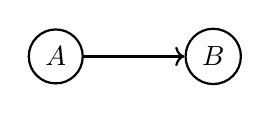
\begin{tikzpicture}[->, node distance=2cm, thick]
      \node[circle, draw] (A) {\(A\)}; \node[circle, draw, right of=A] (B)
      {\(B\)}; \draw (A) -- (B);
    \end{tikzpicture}
  \end{center}
  \item \textbf{Common Response:} Perhaps the effect of vaping on your ateries
  is perfectly benign, but there is some other variable $C$ that causes both
  to occur simultaneously:
  
  \begin{center}
    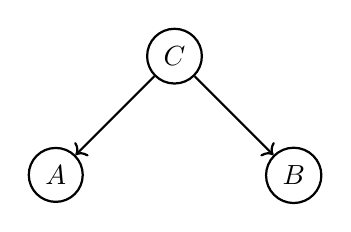
\begin{tikzpicture}[->, node distance=1cm and 1cm, thick]
      \node[circle, draw] (C) {\(C\)}; \node[circle, draw, below left=of C]
      (A) {\(A\)}; \node[circle, draw, below right=of C] (B) {\(B\)}; \draw
      (C) -- (A); \draw (C) -- (B);
    \end{tikzpicture}
  \end{center}
  For example we might have $C=\left[ \text{person smokes cigarettes}
  \right]$. Maybe vapers are disproportionately likely to be cigarette
  smokers, and it's this subset of vapers that drives the association between
  vaping and arterial disease. If this is true, then  quitting vaping woudn't
  decrease your chance of arterial disease.


  \item \textbf{Confounding:} A third variable jointly influences or causes
  both $A$ and $B$. For example, maybe vapers have lower rates of coronary
  artery disease than the general population -- that doesn't mean vaping
  necessarily have a protective effect. For example, maybe the vapers are on
  average younger than the population, and CAD is something that typically
  hapens to old people. In that case, we might observe a spurious relationship
  between $A$ and $B$ due to the effects of some other third variable, 
  $C= \left[ \text{youth} \right]$:
  \begin{center}
    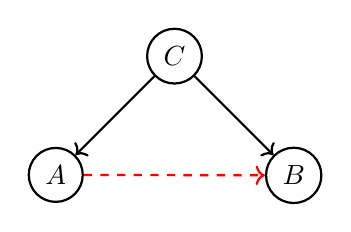
\begin{tikzpicture}[->, node distance=1cm and 1cm, thick]
      \node[circle, draw] (C) {\(C\)}; \node[circle, draw, below left=of C]
      (A) {\(A\)}; \node[circle, draw, below right=of C] (B) {\(B\)}; \draw
      (C) -- (A); \draw (C) -- (B); \draw[dashed, red] (A) --
      (B); % spurious association
    \end{tikzpicture}
  \end{center}
\end{itemize}

What we can say, however, is that if $A$ and $B$ do not have any relationship,
then they are probabilistically independent. In what follows, we will describe
how the hypothesis testing framework can be used to test whether two things
$A$ and $B$ are independent.


This is what tests of association do. They ask the question \textbf{``Are $A$ and $B$
  independent?''} The answer to such tests is always either ``no'' or
``maybe''. They don't give us more information than that.



We need some theory to describe how to do this.

\subsection{Ingredient \#1: The Multinomial Distribution}
Recall that to construct a \textit{binomial} random variable, you flip coins
$n$ times, and count the number of heads. The coin flip only has two outimes.
What if, instead of flipping coin, we rolled a dice with $k$ sides, and
counted the number of times we get $1,2,\ldots,k$? In that case, we get an
example of what is called \demph{multinomial} random variable. To be precise:

\begin{definition}[Multinomial Distribution]
  \label{def:multinomial}
  Consider an experiment with $k$ possible outcomes, labeled $1$ through $k$..
  These outcomes have probabilities $p_{1},\ldots,p_{k}$, respectively. (So
  $p_{1}+\cdots+p_{k}=1$). We repeat this experiment $n$ times, and define
  \begin{equation*}
    X_{i}= \# \text{ of times outcome $i$ occurs in the $n$ trials}
  \end{equation*}
  for each $i=1,\ldots,k$. Then the random vector
  \begin{equation*}
    X = (X_{1},\ldots,X_{k})
  \end{equation*}
  is called a \demph{multinomial random variable} with parameters
  $(p_{1},\ldots,p_{k}) $ and number of trials $n$.
\end{definition}

This is an example of a categorical random variable ($k$ categories). 

Let's do an example with $k=3$.

\begin{example}[One armed bandit]
  \label{ex:one-armed-bandit}
  A single play of a slot machine has three outcomes:
  \begin{itemize}
    \item outcome 1: win nothing
    \item outcome 2: win back your bet
    \item outcome 3: win big
  \end{itemize}
  There is a sticker on the machine which says that these outcomes have
  probabiliites $(p_{1},p_{2},p_{3})=(.5,.3,.2)$. A gambler decides to play
  the game $n=100$ times. For each $i=1,2,3$ let $N_{i}$ be a random variable
  indicating the number of times that outcome $i$ occurred.

  If the sticker is accurate, then the random vector $N=(N_{1},N_{2},N_{3})$
  is a multinomial random variable with parameters
  $(p_{1},p_{2},p_{3})=(.5,.3,.2)$ and $n=100$. Clearly
  \begin{equation*}
    \E\left[N_{i} \right] = np_{i}
  \end{equation*}
  So
  \begin{equation*}
    \E\left[N_{1} \right] = 50
    \quad \text{and} \quad \E\left[N_{2} \right] = 30
    \quad \text{and} \quad \E\left[N_{3} \right] = 20
  \end{equation*}
  After playing the game, suppose gambler gets $N=(43, 35, 22)$. It is
  convenient to arrange this in a table

  \begin{center}
    \begin{tabular}{c|c|c|c}
      Category & 1 & 2 & 3 \\
      \hline
      Observed & 43 & 35 & 22 \\
      Expected & 50 & 30 & 20 \\
    \end{tabular}
  \end{center}
  We expect the observed values to be pretty close to the expected values. But
  if they \textbf{differ substantially}, then we conclude that maybe the sticker isn't
  accurate. In the hypothesis testing framework, sticker represents the null
  hypothesis
  \begin{equation*}
    H_{0}: (p_{1},p_{2},p_{3}) = (.5,.3,.2).
  \end{equation*}
  \Fl{Question:} How do we quantify ``differ substantially''?
  \Fl{Answer:} One sensible way is to consider the following quantity:
  \begin{align*}\label{eq:28}
    \chi^{2} 
    &:= \frac{(43-50)^{2}}{50} + \frac{(35-30)^{2}}{30}+ \frac{(22-20)^{2}}{20}\\
    &= \frac{49}{50}+ \frac{25}{30}+\frac{4}{20}\\
    &\approx 2.01
  \end{align*}
  each term in this sum takes the form
  \begin{equation*}
    \frac{\left( \text{observed}-\text{expected} \right)^{2} }{\text{expected}}.
  \end{equation*}
  The sum in \Cref{eq:28} is always nonnegative. If the observed values are
  close to the expected values, then it is small. Otherwise it is large. So we
  will look at the size of $\chi^{2}$, and make the following determination
  \begin{itemize}
    \item if $\chi^{2}$ is large: we reject the null hypothesis $H_{0}$
    \item if $\chi^{2}$ is small: we ``fail to reject'' the null hypothesis
  \end{itemize}
  
\end{example}



% \begin{example}[Dice activity]
%   We will estimate the distribution of a multinoimial random variable by
%   rolling dice.
%   \begin{itemize}
%     \item Single dice: $(p_{1},\ldots,p_{6}) = (\frac{1}{6},\frac{1}{6},\frac{1}{6},\frac{1}{6},\frac{1}{6},\frac{1}{6}) $
%   Let's let $n=10$. You might get
%   \begin{equation*}
%     X = (1,2,3,1,2,1)
%   \end{equation*}
%   \item Two dice, added up: $(p_{2},p_{3},p_{4},\ldots,p_{12})=(\frac{1}{36},\frac{2}{36},\frac{3}{36},\frac{4}{36},\frac{5}{36},\frac{6}{26},\frac{5}{36},\frac{4}{36},\frac{3}{36},\frac{2}{36},\frac{1}{36})$
% \end{itemize}
  
% \end{example}

\newpage

\section{2025-04-23 | Week 14 | Lecture 33}

\subsection{Ingredient \#2: The Chi-Squared Distribution}

A special kind of gamma distribution:

\begin{definition}[Chi-Squared Distribution]
  \label{def:chi-squared-distribution}
  Let $k$ be a positive integer. A nonnegative random variable $X$ is said to have
  \demph{chi-squared distribution with parameter $d$} if it has pdf
  \begin{equation*}
    f(x) 
    = \left\{ 
      \begin{array}{l@{\quad:\quad}l} \frac{1}{2^{d/2}\Gamma(d/2)}x^{\frac{d}{2}-1}e^{-x/2} & x \geq 0\\ 0& x<0\end{array}\right.
  \end{equation*}
  In other words, if $X$ is a Gamma distributed random variable with
  parameters $\alpha=d/2$ and $\beta=2$. The parameter $d$ is usually called
  the \demph{degrees of freedom} of $X$.
\end{definition}

From left-to-right, here's what this looks like for $d=2$, $d=4$, and $d=12$:
\begin{center}
  \includegraphics[scale=0.15]{images/chi-squared-d2}
  \includegraphics[scale=0.15]{images/chi-squared-d4}
  \includegraphics[scale=0.15]{images/chi-squared-d12}
\end{center}

Using properties of gamma distribution, we have:
\begin{proposition}
  A $\chi^{2}$ random variable $X$ with $d$ degrees of freedom has
  \begin{equation*}
    \E\left[X \right] = \alpha\beta = d \quad \text{and} \quad \Var(X) = \alpha\beta^{2} = 2d
  \end{equation*}
\end{proposition}

The chi-squared distribution plays a central role in statistical inference. It
is completely determined by its degrees of freedom.



\begin{theorem}
  \label{thm:chi-squared-theorem}
  Suppose $X=(X_{1},\ldots,X_{k})$ is a multinomial random variable with
  parameters $p_{1},\ldots,p_{k}$. Define a new random variable $\chi^{2}$,
  called the \demph{chi-squared statistic} by 
  \begin{equation*}
    \chi^{2} := \sum_{i=1}^{k} \frac{\left(X_{i}-np_{i}\right)^{2}}{np_{i}}.
  \end{equation*}
  Then $\chi^{2}$ has approximately chi-squared distribution with $k-1$ degrees of
  freedom (as long as  $np_{i}\geq 5$ for all $i=1,\ldots,m$).
\end{theorem}

\subsection{The goodness-of-fit test}

With ingredients \#1 and \#2, we can formulate what is called a ``goodness of
fit test''. This isn't quite what we set out to do (i.e., we want to do
\textit{tests of association}), but it's a good first step. Goodness-of-fit
tests are described in detail in chatper 14.1 of the textbook.

In \cref{ex:one-armed-bandit} (one armed bandit), we considered a game with three outcomes, 1,2,
and 3 with unknown probabilities $p_{1},p_{2},$ and $p_{3}$. Our null
hypothesis was that
\begin{equation*}
  H_{0} : (p_{1},p_{2},p_{3})=(0.5,0.3,0.2)
\end{equation*}
and the alternative hypothesis is
\begin{equation*}
  H_{1}: (p_{1},p_{2},p_{3})\neq(0.5,0.3,0.2).
\end{equation*}
We played the game 100 times. Our data is summarized in the following table:
\begin{center}
  \begin{tabular}{c|c|c|c}
    Category & 1 & 2 & 3 \\
    \hline
    Observed & 43 & 35 & 22 \\
    Expected & 50 & 30 & 20 \\
  \end{tabular}
\end{center}
In this table, the expected values were calculated assuming the null
hypothesis that was true. The chi-squred statistic
is
\begin{align*}\label{eq:28}
  \chi^{2} 
  &:= \frac{(43-50)^{2}}{50} + \frac{(35-30)^{2}}{30}+ \frac{(22-20)^{2}}{20}\\
  &= \frac{49}{50}+ \frac{25}{30}+\frac{4}{20}\\
  &\approx 2.01
\end{align*}
Recall that we reject the null hypothesis if $\chi^{2}$ is big, and we fail to
reject the null hypothesis if $\chi^{2}$ is small.


\Fl{Question:} So is $2.01$ big enough to reject $H_{0}$?

\Fl{Answer:} Let's compute a $p$-value, which if you recall is the probability
of observing results at least as extreme as you observed, assuming the null
hypothesis is true.

By \cref{thm:chi-squared-theorem}, we know that the statistic has a
chi-squared distribution with 2 degrees of freedom.

Therefore our $p$-value is
\begin{align*}
  p\text{-value } 
  &= \P\left[\chi^{2}\geq 2.01\right]\\
  &= \int_{2}^{\infty} \frac{1}{2}e^{-x/2} &&\text{by \cref{def:chi-squared-distribution} } \\ 
  &= 0.366
\end{align*}


In other words, if the null hypothesis were true, we would expect to see our
chi-squared statistic be 2.01 or greater about  $37\%$ of the time. That's
pretty common, so we \textbf{fail to reject} the null hypothesis.
\begin{center}
  \includegraphics[scale=.15]{images/chi-sq-shaded}
\end{center}

The test that we just did is called a goodness of fit test. These are
described in chapter 14.1 in the textbook.



\newpage
\section{2025-04-25 | Week 14 | Lecture 34}

The example in this lecture is based on a very nice chi-squared tutorial by
Caitlin Light, available here: \url{https://www.ling.upenn.edu/~clight/chisquared.htm}


\subsection{Tests of Association, Revisted}

We now have the things we need to test whether two things are independent or
not.


\begin{definition}
  A \demph{contingency table} is a matrix of with rows labeled as group 1,
  group 2, and so forth, and columns labeled as outcome 1, outcome 2, etc. The
  entries of the matrix are COUNTS: the $(i,j)$-th entry is the number of
  times that group $i$ experience outcome $j$.
\end{definition}


For example, puppose we have a population of $n=54$ students, which we divide
up according two to factors
\begin{enumerate}[(i)]
  \item whether they attended class regularly or not
  \item whether they pass the class exam or not
\end{enumerate}
Then our contingency table is

\begin{equation}\label{eq:table-of-observed-values}
  \begin{tabular}{l|cc}
    & \textbf{Pass} & \textbf{Fail} \\
    \hline
    \textbf{Attended} & 25          & 6            \\
    \textbf{Skipped}  & 8           & 15           
  \end{tabular} 
\end{equation}
This is the \demph{table of observed values}. We usually augment the table
with ``marginal totals'', like so:


\begin{center} 
  \begin{tabular}{l|cc|c}
    & \textbf{Pass} & \textbf{Fail} & \textbf{Total} \\
    \hline
    \textbf{Attended} & 25 & 6  & 31 \\
    \textbf{Skipped}  & 8  & 15 & 23 \\
    \hline
    \textbf{Total}    & 33 & 21 & 54
  \end{tabular}
\end{center}


The null hypothesis is
\begin{equation*}
  H_{0}= \text{ attendence and passing are independent}
\end{equation*}
and the alternative hypothesis is
\begin{equation*}
  H_{1} = \text{ there is a relationship between attendence and passing.}
\end{equation*}


Let $p$ denote the probability that a student regularly attends class, and let
$q$ denote the probability that a student passes the final exam.

\fl{Important:} We do not know the true value of $p$ and $q$. But we can
estimate them using the marginal row and column sums from the table:
\begin{equation*}
  p \approx \frac{31}{54} \quad \text{and} \quad q\approx \frac{33}{54}
\end{equation*}


\Fl{Question:} What are the expected values of the table, assuming the null
hypothesis is true?


Under the null hypothesis, we can multiply probabilities, e.g., so that the
probability that a student both regularly attends class AND passes the exam is
about $pq$. Therefore, since there are $n$ students,
\begin{align*}
  &\E\left[\text{\# of students who attend regularly AND pass the exam}\right] \\
  &= n \P\left[\text{a randomly-selected student attends regularly AND pass the exam} \right]\\
  &= n \P\left[\text{attends regularly}\right] \P\left[\text{passes the exam} \right]\\
  &= npq
\end{align*}

Similar calculations gives us the following table of expected counts:
  \begin{center}
    \begin{tabular}{l|cc}
      & \textbf{Pass} & \textbf{Fail} \\
      \hline
      \textbf{Attended} & $npq$          & $np(1-q)$            \\
      \textbf{Skipped}  & $n(1-p)q$           & $n(1-p)(1-q)$            
    \end{tabular}
  \end{center}
  and plugging in the values $n=56$ and our approximations  $p\approx
\frac{31}{54}$ and $q\approx \frac{33}{54}$ gives

\begin{equation}\label{eq:table-of-estimated-expected-values}
  \begin{tabular}{l|cc}
    & \textbf{Pass} & \textbf{Fail} \\
    \hline
    \textbf{Attended} & $18.9$          & $12.1$            \\
    \textbf{Skipped}  & $14.1$           & $8.9$            
  \end{tabular}
\end{equation}
This is the \demph{table of estimated expected values.} Using the values of
\Cref{eq:table-of-observed-values,eq:table-of-estimated-expected-values}, we
compute a chi-squared statistic:
\begin{align*}
  \chi^{2} 
  &= \sum_{\text{all table entries}} \frac{\left( \text{observed
    value} - \text{expected value} \right)^{2} }{ \text{expected value}} \\
  &= \frac{\left( 25-18.9 \right)^{2} }{20.2}+ \frac{(6-12.1)^{2}}{12.1}+ \frac{\left( 8-14.1 \right)^{2} }{14.1}+ \frac{\left( 15-8.9 \right)^{2} }{8.9}\\
  &= 11.7
\end{align*}

By \cref{thm:chi-squared-theorem}, we know that $\chi^{2}$ has a chi-squared
distribution. The degrees of freedom thing isn't so clear from that theorem,
but when working with a contingency table, the degrees of freedom is given by the equation
\begin{equation*}
  (\text{number of rows} -1)\times (\text{number of columns} -1)
\end{equation*}
which in our case, for a $2\times 2$ table, is just 1.


Thereore, using \cref{def:chi-squared-distribution}, the p-value is
\begin{align*}
  p \text{-value} 
  &= \int_{11.7}^{\infty} \frac{1}{\sqrt{2\pi}} x^{-\frac{1}{2}}e^{-x/2}dx\\
  &=0.0006
\end{align*}
In other words, if attending and passing were independent, we would see
results this extreme only 0.06\% of the time. This is very small, so we reject
the null hypothesis. Our conclusion is that attendance and passing the final
exam are \textbf{not independent}, i.e., that there is a relationship between
them.

At this point we are tempted to conclude that regularly attending class
increases your chance of passing the final exam. This seems obvious and is
certainly consistent with the data. But it's not a conclusion that follows
from the test that we did. The test only told us that these two things things
probably have some relationship; it doesn't give us information about the
nature of that relationship.

\section{2025-04-30 | Week 15 | Lecture 35}

Topic: Finding a ``best fit line'' using ordinary least squares linear
regression. Handwritten notes.

\section{2025-05-02 | Week 15 | Lecture 36}

Topic: the simple linear regression model with mean-zero gaussian errors.
Handwritten notes.

\newpage
\section{2025-05-05 |  Week 16 | Lecture 37}

\subsection{Odds}

Suppose $A$ is an event with probability $p$. The \demph{odds} or \demph{odds
  ratio} is the fraction
\begin{equation*}
  \frac{p}{1-p}.
\end{equation*}
The idea of \textit{odds} (which can be any positive number) is older than that
of probability (which can only be betwen 0 and 1).  When outcomes are equally
likely, the \textit{probability} $p$ is understood to be
\begin{equation*}
  \frac{\text{number of favorable outcomes}}{\text{total number of possible outcomes}},
\end{equation*}
whereas \textit{odds} is
\begin{equation*}
  \frac{\text{number of favorable outcomes}}{\text{number of unfavorable outcomes}}
\end{equation*}
For example, the probability of rolling a 6 on a dice is $1/6$, and the odds
is $1/5$. In some sense knowing the odds gives you the same amount of
information as knowing the probability (since if you know one, you can compute
the other), but the interpretation is different. For example, odds of $1/5$
tell us that failure is 5 times more likely than success. We would say the
odds are ``5-to-1 against'', or ``1-to-5 against''.

Odds are commonly used in betting situations. Odds is useful in betting
situations because it gives a measure of the player's advantage. The first
mathematical text on probability was Girolamo Cardano's 15-page text ``The
Book on Games of Chance'' written in 1564 (though first published only a
century later). Much of the work is in terms of ``odds'', and he appears to be
the first to formulate probability in terms of the ratio of favorable outcomes
to total outcomes.


\subsection{Logistic Regression}
Suppose we have a numerical predictor variable $x$, which can take a range of
values, and we are interested in a binary response variable $Y$, which can
take only values $0$ and $1$. That is $Y$ provides a binary classification.
For example,
\begin{equation*}
  x= \text{ mileage of car} \quad \text{and} \quad Y = \left\{ \begin{array}{l@{\quad:\quad}l} 1 &\text{if the car needs
        maintenance} \\ 0& \text{if the car doesn't need maintenance} \end{array}\right.
\end{equation*}

For the wiki problem \url{https://en.wikipedia.org/wiki/Logistic_regression#Example}, we have data
\begin{center}
  \resizebox{.8\textwidth}{!}{
    \begin{tabular}{c|cccccccccccccccccccc}
      \textbf{Hours ($x_k$)} & 0.50 & 0.75 & 1.00 & 1.25 & 1.50 & 1.75 & 1.75 & 2.00 & 2.25 & 2.50 & 2.75 & 3.00 & 3.25 & 3.50 & 4.00 & 4.25 & 4.50 & 4.75 & 5.00 & 5.50 \\
      \hline
      \textbf{Pass ($y_k$)}  & 0    & 0    & 0    & 0    & 0    & 0    & 1    & 0    & 1    & 0    & 1    & 0    & 1    & 0    & 1    & 1    & 1    & 1    & 1    & 1
    \end{tabular}}
\end{center}

\begin{center}
  \includegraphics[scale=0.2]{images/logistic-example}
\end{center}


For this setting, it doesn't make sense to try to fit a best line, since there
are only 2 possible $y$-values: 0 and 1. instead, we consider the probability
$p(x) = \P\left[Y=1 \right]$, which increases from $0$ to $1$ as the mileage
$x$ increases.


The \demph{logistic function} is the function $f(x) = \frac{e^{C+Dx}}{1+e^{C+Dx}}$, where
$C,D\in \R$. An example when $D>0$ is the following increasing function
\begin{center}
  \includegraphics[scale=.3]{images/logistic}
\end{center}

In \textit{logistic regression}, we make the \textbf{assumption} that the
logarithm of the odds is approximately linear, i.e, that
\begin{equation}\label{eq:30}
  \log\left(\frac{p(x)}{1-p(x)} \right)  \approx C+Dx
\end{equation}
for some choice of $C$ and $D$.  This is equivalent to assuming that the
probability of, say, engine failure is approximated by the logistic function,
so we assume that
\begin{equation}\label{eq:29}
  p(x) = \frac{e^{C+Dx}}{1+e^{C+Dx}}
\end{equation}
for some choice of real numbers $C$ and $D$. 


When we found a ``best fit line'' for some data, recall that we looked for
values of $C$ and $D$ which minimized the magnitude of the error vector
\begin{equation*}
  e = (e_{1},e_{2},\ldots,e_{n})
\end{equation*}
where $e_{i} = y_{i} - (C+Dx_{i})$ is the vertical distance between our
observed data and what is predicted by the line $y=C+Dx$.

For logistic regression, we do something similar, but instead of minimizing
the sum of squares $\norm{e}^{2}=e_{1}^{2}+e_{2}^{2}+\ldots+e_{n}^{2}$, we
instead seek to minimize something much more complicated: \demph{the
  surprisal}.

Consider the single data point $(x_{i},y_{i})$. Here $y_{i}$ is either 0 or 1,
but $x_{i}\in \R$.

According to the model given in \cref{eq:29}, for any choice of model
parametesr $C$ and $D$, the predicted probability that $y_{i}=1$ is
\begin{equation*}
  p(x_{i}) = \frac{e^{C+Dx_{i}}}{1+e^{C+Dx_{i}}}
\end{equation*}
Let's call this number $p_{i}$ and observe that $0<p_{i}<1$.
The \demph{surprisal} (or ``\demph{log loss}'') at the data point
$(x_{i},y_{i})$ is the quantity
\begin{equation*}
  \ell_{i} 
  := - \log\left( p_{i}^{y_{i}}(1-p_{i})^{1-y_{i}} \right) 
  = \left\{ 
    \begin{array}{l@{\quad:\quad}l} \log(\frac{1}{p_{i}}) & y_{i}=1\\ \log\left(\frac{1}{1-p_{i}} \right)  & y_{i}=0 \end{array}\right. 
\end{equation*}

Observations
\begin{itemize}
  \item $\ell_{i}>0$
  \item $\ell_{i}$ really does measure ``surprise'' in some sense. For
  example, if $p_{i}\approx 0$  and $y_{i}=0$, then $\ell_{i} \approx
  \log(1)=0$. But if $p_{i} \approx 1$ and $y_{i}=0$, then $\ell_{i}\approx
  \log(\text{big number})=\text{big}$. Bigger values means there is more
  discrepancy between what is predicted by the model and what is observed.
\end{itemize}
The \demph{total loss} is the sum of all the surprisals:
\begin{equation*}
  T(C,D) = \ell_{1}+\ell_{2}+\ldots+\ell_{n}
\end{equation*}
Observations
\begin{itemize}
  \item $T$ is a complicated function of the parameters $C$ and $D$.
  \item Each choice of $C, D$ correspond to some model from the family \cref{eq:29}
  \item When $T(C,D)$ is large, the observed data
  $(x_{1},y_{1}),\ldots,(x_{n},y_{n})$ would be unlikely to occur for that
  choice of $C$ and $D$. But if $T(C,D)$ is close to zero, then the model
  would be more likely to produce data like what was observed.
  \item In this way the quantity $T(C,D)$ may be regarded as a ``distance''
  between your observed data and the model with parameters $C,D$. The goal is
  to find the values of $C,D$ which minimize this distance---these will give
  you the ``best'' model for your data.
\end{itemize}
In logistic regression, the goal is to try to find the values of $C,D$ which
minimize the $T(C,D)$. This cannot reasonably be done by hand, as the function
$T$ is complicated enough that we don't have closed form solutions. Instead,
more typically, one will use software to check many values of $C$ and $D$ and
use whichever appears to give you the smallest $T(C,D)$. Actual
implementations use sophisticated heuristics to do this.

For the wiki problem, the best $C$ and $D$ we get are $C \approx -4.1$ and
$D\approx 1.5$, this gives the ``best model'' to be
\begin{equation*}
  p_{\rm best}(x) = \frac{e^{-4.1+1.5x}}{1+e^{-4.1+1.5x}}
\end{equation*}
and which gives the curve graphed above.

This model can then be used to make predictions.For example, if you study 3
hours, your probability of passing is predicted to be
\begin{equation*}
  p_{\rm best}(3) = \frac{e^{-4.1+1.5(3)}}{1+e^{-4.1+1.5(3)}} \approx 0.6.
\end{equation*}


The example we have worked has assumed that there is only one explanatory
variable $x$. This restriction isn't essential to the theory. Suppose instead that
we have 2 explanatory variables, $x$ and $w$. Now, instead of \cref{eq:30} we have
\begin{equation*}
  \log\left(\frac{p(x)}{1-p(x)} \right) \approx C+Dx+ Ew
\end{equation*}
We have added a new parameter $E$. So now we must minimize the total loss over
all $C,D,$ and $E$, rather than just over all $C$ and $D$. Nothing else
changes. You can add as many explanatory variables as you like.

If you have a dataset with lots of possible explanatory variables, how do you
know which ones to include and which to exclude from a logistic regression
analysis? For example: $Y$ indicates whether a surgery patient experiences
complications due to surgery (assume same type of surgery). Possible
explanatory variables
\begin{itemize}
  \item patient age, sex
  \item surgical device type 
  \item year that surgery was performed
  \item attending physician
  \item preexisting conditions
  \item innumerable other risk factors
\end{itemize}
If you include all of them, you get results that may be overfitted
and may be hard to interpret. One option is to repeatedly do many analyes with
different subsets of your explanatory variables, with some penalty applied so
that models with fewer parameters are preferred (see, e.g. the Bayesian
Information Criterion (BIC) score). These are related to goodness of fit tests
like the ones we did for the skittle distribution.


\newpage



\section{Other stuff}

\begin{example}
  If a ray of light hits a flat a matte surface in 2D, then it will bounce off
  at a random angle. Let $\theta$ be the angle from the normal vector to the
  surface. Then $\theta$ is a random variable which can take values in the
  interval $[-\frac{\pi}{2},\frac{\pi}{2}]$.

  Some law from physics says that the relative likelihood that a ray bounces off
  at an angle $u$ from the normal vector is proportional to the length of the
  following vector

  \begin{center}
    \includegraphics[scale=0.05]{images/light-ray-law}
  \end{center}

  This vector has length $2\cos(u)$.


  \textbf{Question:} What is the probability that the light ray bounces off at an angle between less than
  45 degrees from the surface?


  \textbf{Approach:} We first will compute the probability density function $f_{\theta}(u)$. We know that
  \begin{equation*}
    f_{\theta}(u) \text{ is proportional to } 2\cos(\theta)
  \end{equation*}
  or in other words, that
  \begin{equation*}
    f_{\theta}(u) = 2C\cos(\theta)
  \end{equation*}
  where $C>0$ is an unknown constant.
  
  We also know that
  \begin{equation*}
    \int_{-\frac{\pi}{2}}^{\frac{\pi}{2}} f_{\theta}(u)du = 1
  \end{equation*}

  Using these two facts, we can conclude that
  \begin{equation*}
    f_{\theta}(u) = \frac{1}{2}\cos(\theta).
  \end{equation*}

  We want $\P\left[|\theta|>\frac{\pi}{4}  \right]$. We can write this as
  \begin{equation*}
    \P\left[\theta\in (\frac{\pi}{4},\frac{\pi}{2}] \right] + \P\left[\theta\in [-\frac{\pi}{2}, \frac{\pi}{4}) \right]
  \end{equation*}
  By symmetry, these are equal so we have
  \begin{equation*}
    \P\left[|\theta|>\frac{\pi}{4}  \right] = 2     \P\left[ \frac{\pi}{4}<\theta \leq \frac{\pi}{2} \right]
  \end{equation*}
\end{example}
\newpage



\begin{example}[Law of total probability]
  Deal two cards. Let $F$ be the event that the first card is an ace. Let $G$ be the event that the
  second card is an ace.

  Use law of total probability to show that $\P\left[G \right] = \frac{4}{52}$.
  \begin{align*}
    \P\left[G \right] 
    &= \P\left[F \right]\P\left[G\mid F \right] + \P\left[F^{c} \right]\P\left[G\mid F^{c} \right]\\
    &= \frac{4}{52}\cdot \frac{3}{51} + \frac{48}{52} \cdot \frac{4}{51}\\ 
    &= \frac{4}{52} \left[ \frac{3}{51}+\frac{48}{51} \right]\\ 
    &= \frac{4}{52}
  \end{align*}
\end{example}

\begin{example}[Flipping hidden coins]
  Probability can be 
  \begin{enumerate}[(a)]
    \item A gambler has a fair coin and a 2-headed coin in his pocket. Without looking, he draws one of the
    coins at random from his pocket. When he flips it, it comes up heads. What's the probability that
    it's the fair coin?
    \item Suppose that he flips the same coin a second time and, again, it shows up heads. Given the
    information that he has flipped heads twice in a row with this coin, what is the probability that
    it's the fair coin?
    \item Suppose he flips it a third time and it shows up heads again. Given the information that he
    has flipped the heads three times in a row with this coin, what is the probability that it's the
    fair coin?
    \item He flips it yet one more time, and this time it comes up tails. Given this information,
    what's the probability that it's the fair coin?
  \end{enumerate}
\end{example}


 

\end{document}

